
\chapter{Community detection}
\label{chap:community detection}
%\todo{Mpve spinglass to end}

This chapter moves to the next level of analysis, network communities, meso-scale structures in the network. I will combine community detection with GSA (section~\ref{sec:Gene set tests}) to test if  PSP network communities are associated with intelligence or educational attainment. We will develop a general strategy to decide which community detection methods to use. 

Having discussed the genetics of differences in intelligence and educational attainment (section~\ref{sec:intelligence intro recent gwas}) and reviewed the insights gained from Gene Set Analysis (GSA) (section~\ref{sec:Gene set tests}) we can see that GSA provided evidence for the involvement of the brain, the synapse and neurogenesis as biological mechanisms that may underlie these traits. We also saw that GSA is limited by the choice of curated gene sets and it is hard to `discover' new gene sets. A prominent network orientated GSA methods paper called for data driven gene sets\cite{lamparter2016fast}. Given that the synaptic proteome is inherently modular (section~\ref{sec:Introduction finding communities in protein protein interactions}) and the previous success of clustering algorithms in the synapse we test whether GSA and community detection can illuminate the genetics of intelligence as a paradigmatic case. 





\section{Network communities}
\label{sec: community detection intro gsa}


Communities, sub-graphs with dense interactions between community members and sparser connections to the rest of the graph (figure~\ref{fig:communities}), \cite{newman2012communities},\cite{fortunato2016community},\cite{girvan2002community} are the most well studied large-scale structure in networks\cite{newman2012communities}.  Absent from random graphs they are of interest because they may represent function units: in human and animal social networks they have been shown to correspond to real world groupings, and these assignments can be discovered using the pattern of connectivity of the vertices\cite{adamic2005political},\cite{zachary1977information}\cite{newman2018networks}\footnote{add page}.  An example of a community would be a group of friends in a social network; in the synaptic protein network, communities may represent functional modules\cite{pocklington2006proteomes},\cite{mclean2016improved} and could be used as data generated gene sets for competitive GSA.  

\begin{figure}
    \centering
    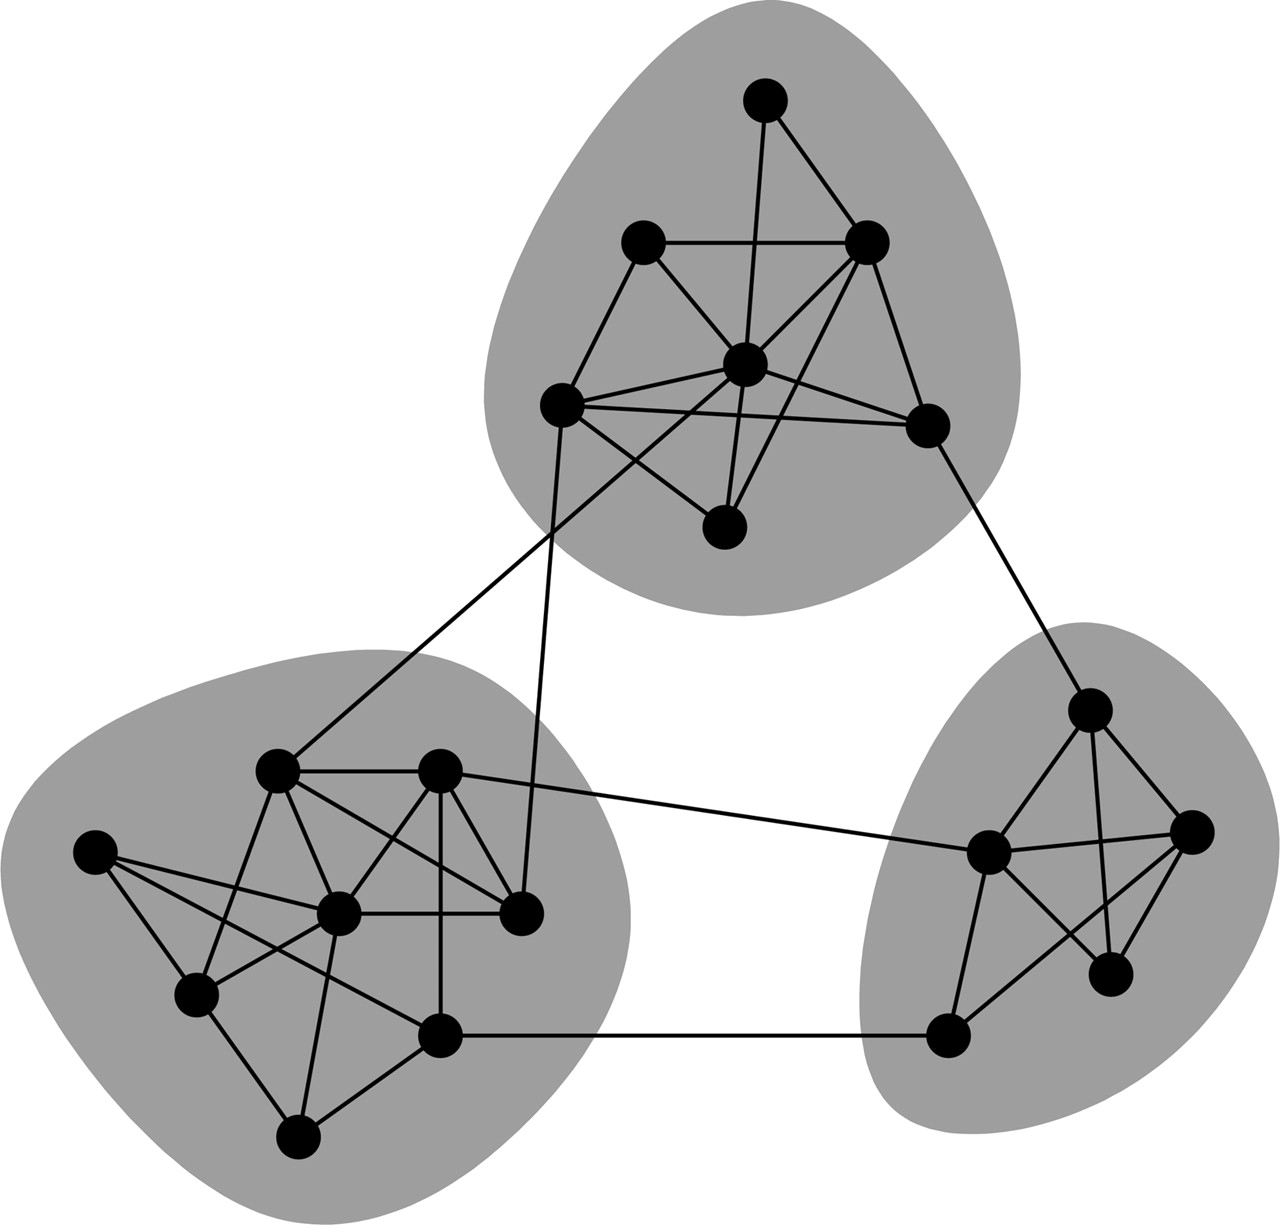
\includegraphics[width=\textwidth]{images/chapter_community_detection/creative_commons/F1large.jpg}
    \caption[Figure of three communities]{Line drawing of three communities showing dense connections within the communities (shaded) and fewer connections between communities}
    \tiny Creative commons for attribution see \url{https://commons.wikimedia.org/wiki/File:Network_Community_Structure.svg}
    \label{fig:communities}
\end{figure}

 Community detection methods when applied to smaller, earlier synaptic protein networks with over-representation GSA have shown differential enrichment of disease and Gene Ontology terms in particular communities\cite{pocklington2006proteomes},\cite{mclean2016improved}.  One study that used over representation GSA to test communities from protein-protein interaction networks used the results from GWA studies to add to the list of disease associated genes for seventy different disorders\cite{ghiassian2015disease}. Their analysis did not however use all the information available in summary GWAS statistics, the protein-protein interaction network was generated using evidence other than direct interaction (such as co-expression) and the network was not representative of the tissues affected by the diseases or traits under consideration\cite{ghiassian2015disease}.

Different tissues will contain different proteins and so the protein interaction network will have different nodes and edges. Vertex (node) statistics such as degree will be different and community detection algorithms may give different results.

The hierarchical divisive edge betweenness community detection method (Girvan–Newman algorithm) \cite{girvan2002community} has been used (section~\ref{sec:Newman and Girvan}) to discover communities in the protein-protein interaction graph of the NRC/MASC complex (248 edges, 105 nodes)\cite{pocklington2006proteomes}. This method has the advantage that the number of communities does not have to be determined in advance, the optimum level to stop the division is the maximum of an objective function, the modularity ($Q$), which determines the quality of the division of a network into communities\cite{girvan2002community}. 
%  Modularity had previously been introduced in the context of categorical assortativity.  Modularity is a measure of the difference between the number of edges found between members of a community and the expected number of edges given the degree of the network. In nominal assortativity\textcolor{red}{A} there were two groups, one that had the property and one that did not; an alternative way to see this is as two communities (cf adamcic). This is calculated using a random model of edge generation, the configuration model, where the degree of nodes is fixed and the edges assigned at random\cite{fortunato2016community}. 
 
\subsection{Modularity}
\label{sec:modularity introduction}
Modularity ($Q$) was used as a measure of nominal assortativity (equation~\ref{eq:categorical assortativity}, section~\ref{sec:assortativity}) the extent to which vertices that share a property are linked. A natural extension is as a measure of the quality of the division of the network into multiple groups, communities, where community membership is the property that nodes possess that maximises the modularity. 

 The most common method of community detection seek to maximise an objective function typically the modularity (see section~\ref{sec:modularity introduction} and Eq(\ref{eq: modularity A-kk delta group})) over possible partitions of the network to obtain non-overlapping groupings of the nodes\cite{newman2013spectral}. Alternately a statistical model can be used to find the community allocation most likely to generate the network although modularity and maximum likelihood approaches have been shown to be equivalent\cite{newman2016equivalence}. Modularity maximisation is computationally hard (NP complete\cite{brandes2007modularity}) and a number of heuristics have been described to provide approximations to the optimal modularity\cite{newman2013spectral}. Community detection algorithms also vary by being divisive or agglomerative and hierarchical (where smaller clusters are nested in larger ones) or partitional (where the best division of the network is sought without regard for hierarchy\cite{reichardt2006statistical}). 

 With increasing graph size some algorithms can become unstable, give rise to improbable community sizes, or become prohibitively computationally expensive\cite{pocklington2006proteomes},\cite{mclean2016improved}. 
McLean et al.\cite{mclean2016improved} described a parallelised implementation of the edge betweenness algorithm used previously on the NRC-MASC complex\cite{pocklington2006organization} and found it to be prohibitively slow with large networks. With a contemporary (2016) version of the human PSD proteome (V=1312, E=8031) the algorithm took 14 days (20,160 minutes) and the estimated completion time for a sequential implementation was 26 days (37,889 minutes). For all edge betweenness algorithms including parallelised implementations there is a steep inflection point in running time at around 4,000 edges (figure 1 in the manuscript\cite{mclean2016improved}).

One method of community detection that scales well with network size makes use of the spectral properties of the matrix representations of the network\cite{newman2013spectral}.  The network can be recurrently partitioned using the sign of the leading eigenvector of the modularity matrix\cite{newman2013spectral}.  McLean et al \cite{mclean2016improved} provide an implementation of this algorithm, which we will use in this chapter, along with the random walk and edge betweenness algorithms optimised for computers with multiple cores. Examining the performance of these algorithms on an earlier network model of the human post synaptic density (PSD) proteome (V=1,312, E=8,031) they found that the spectral clustering method with a fine-tuning step provided the best performance, measured by running time, community size and differential functional enrichment. 

In this chapter I will first try to find the best community detection algorithm for the larger (V=3,457) PSP. This will expand upon the analysis of McLean\cite{mclean2016improved} et al. as I will look in particular for algorithms that produce communities well suited for gene set analysis. The size of the communities generated is important as confounding effects can occur with large gene sets\cite{de2016statistical} and there may also be an optimum size of cohesive communities \cite{leskovec2009community}. On the other hand large numbers of small communities will result in sets dominated by the most significant genes and an increased penalty for multiple testing with a resultant decrease in power in analysing population GWAS-GSA. Algorithms that are prohibitively slow on networks of over 3000 nodes will not be suitable and algorithms that are `self-tuning', lacking additional parameters or the necessity to determine community size in advance, are preferred as they simplify study design. If there are not clear default or optimal parameters settings then each different setting could (should?) be regarded as a different test increasing type I error. 

Prospective algorithms in addition should be readily implementable and produce communities that `look right' and generally correspond to functional units. 


\section{Communities}
\label{sec:alternate intro}

Given that there are a number of available community detection algorithms it is likely that there is not one that is clearly superior\cite{aldecoa2013exploring}. Before testing communities using GSA we have to decide on an appropriate community detection algorithm or algorithms.

\subsection{Assessment of communities}
\label{sec:assessment of communities}
A number of benchmarks for community detection algorithms exist including the use of networks where we know the community allocation of the vertices (`Ground truth'\cite{yang2015defining}, examples include Zachary's Karate club\cite{zachary1977information}) or the use of benchmark networks which can be simple (Girvan-Newman, 128 nodes, four communities\cite{girvan2002community}) or derived from a more realistic generative model (Lancichinetti–Fortunato–Radicchi (LFR)\cite{lancichinetti2008benchmark}). Although they have been used to determine the `best' algorithm under different circumstances (\cite{yang2016comparative}) they have been less widely reported to select an algorithm for a particular the context of network analyses. The reason is probably that these analyses of algorithms\cite{yang2016comparative}, \cite{aldecoa2013exploring} are very involved but a simple procedure is to choose the LFR benchmark most similar to the network one is studying and assess algorithm performance on it in terms of performance measures and community size. 

Looking at the performance of community detection algorithms on ground truth communities Yang and Leskovec (2015) describe the usual process of assessing community detection performance. It bears quoting at length:

``Generally, after some community detection algorithm identifies communities based on the network structure, the essential next step is to interpret the communities by identifying a common external property or a function that the members of a given community share and around which the community organizes. \textit{For example, given a protein–protein interaction network of a cell, one first identifies communities based on the structure of the network and then examines that these communities correspond to real functional units of a cell}\cite{yang2015defining}\footnote{italics mine}.'' 

This has been the standard approach and has the obvious disadvantage that one only finds what one expects to find. In the example above one must \textit{know} the ``real functional units of the cell''. There is no chance to find new structure or organisation although it is well recognised that valuable structure can be discovered that differs from `ground truth'\cite{fortunato2016community}\footnote{p056104-8 para. 1; division of karate club into seven groups see also discussion of Girvan–Newman algorithm}. 

In studies of community detection in biological networks\todo{give examples} Gene Ontology definitions\cite{mclean2016improved}, Gene RIF, gene lists of gene disease associations (GDA) such as OMIM \cite{hamosh2005online}\footnote{(application \cite{ghiassian2015disease})}, ClinVar \cite{landrum2016clinvar}\footnote{application \cite{luck2020reference} ref 46}, CTD (Comparative Toxicogenomics Database) \cite{davis2019comparative}\footnote{application \cite{baker2012geneweaver}}, dbGAP \cite{tryka2014ncbi} DisGeNET \cite{pinero2020disgenet} \cite{pinero2016disgenet} and GWAS catalog\footnote{note to self -sic}\cite{welter2014nhgri} have been used  to assess whether the community detection algorithm is returning `natural' communities in the belief that a community enriched for these terms represents a functional unit, an entity that differs from a random selection of the elements that make up the network. 

There are a number of assumptions implicit in this including: that Gene Ontology or disease terms are precisely mapped, that a module has one function and that we know or can enumerate all functional units in a tissue (based on Gene Ontology or another repository).

One of the problems with this approach is that we know that these lists of genes do not correspond exactly with the findings of large scale population genetic studies. For example in DisGeNET over 1,000 genes are associated with schizophrenia from curated sources and the total number of genes found in the database is 1,700\cite{pinero2020disgenet}. This represents approximately 8.5\% of protein encoding genes in the genome \cite{ezkurdia2014multiple}. This contrasts with 341 genes found in the Psychiatric Genomics Consortium–Schizophrenia Workgroup (PGC–SCZ) genome wide association study \cite{ripke2014biological}. These genes include those found in animal models or drug targets or may be found in diseases associated with schizophrenia. Using such a heterogenous group may lead to a set of genes with a limited connection to schizophrenia appearing to have a significantly enriched association).  

There is also the issue of the definition of disease.  DisGeNET disease refers to `actual diseases, disease symptoms and abnormal phenotypes that are observed as disease manifestations as well as normal traits and phenotypes that are currently explored in large scale Genome Wide Association studies (GWAS)\cite{pinero2020disgenet}'. Statements therefore about where diseases are placed within the interactome \cite{barabasi2016network},\cite{ghiassian2015disease} and their properties may refer to a number of different entities. It would be better to address specific diseases or sets of diseases and differentiate between genetic variation associated with them, gene expression in a specific phase of the disorder or the genes targeted by common therapies. Finally all of the genes in these lists are scored equally in over-representation analyses whether they have a very strong association with the disorder or a weak one. Using information from GWA catalog to populate a gene disease association list does not provide the full polygenic signal from a group of genes found in summary GWA data. 

One way to test the clustering algorithms utility is to see whether it discovers communities that are associated with a disease or trait in population studies where the disease or trait is operationalised as much as possible (GWAS)\cite{cai2020reviewing}\cite{van2013power}. By using competitive Gene Set analysis using GWA study data as implemented in programs such as MAGMA\cite{de2015magma} or PASCAL\cite{lamparter2016fast} we overcome the problems of thresholding and in addition we may discover new insights into the subject of the GWA study.

We will still need some criteria to decide upon which algorithm to use in this GSA paradigm. Before turning to this we have to introduce the community detection methods. 

\todo{also the difficulty in choosing the appropriate metric for GO analysis eg p value, fold change, proportion of community}




\section{Choice of community detection algorithm}
\label{sec:choice of community detection algorithm}
Given the number of community detection algorithms that are described it is likely none is optimal\cite{aldecoa2013exploring}. The Girvan-Newman (GN) benchmark \cite{girvan2002community} is a standardised benchmark with 128 nodes and four communities but is regarded as being too simple\cite{aldecoa2013exploring}. One limitation is that communities and degree are similar and the more demanding Lancichinetti–Fortunato–Radicchi (LFR)\cite{lancichinetti2008benchmark} allows scale free community size and degree(section~\ref{sec:LFR benchmark}). The other main way to assess algorithms is to compare communities with networks in which the `ground truth' (or metadata associated with the nodes) is known\footnote{leaving aside for now the question of what constitutes ground truth}\cite{leskovec2010empirical}.

Algorithms that perform well on small data sets often do not scale to larger networks\cite{girvan2002community},\cite{mclean2016improved},\cite{yang2016comparative}. In addition we would like to partition the network into communities that are both topologically robust but make sense biologically. It is hard to be prescriptive about what this means it is essentially to reject the implausible. For example, We have an intuition that the PSP network consists of more than three components, if it were divided by an algorithm into three components we would expect these would in turn have identifiable subdivisions. Biological plausibility\cite{pocklington2006organization} has been used to choose between algorithms and set parameters. At larger scale the best I can do is to reject the implausible or impracticable (see below). 

The goal of this chapter is to combined Gene set analysis (GSA) with community detection to provide data generated gene sets. GSA can be biased by very large and very small groups\cite{de2016statistical} and there are arguments that community sizes in real world networks tend to follow power law distributions (or at least heavily right skewed distributions)\cite{lancichinetti2008benchmark} or conform to an optimum size\cite{leskovec2010empirical}. A reasonable place to start would be community detection methods that give `good enough' communities on the PSP network. 


An ideal community detection algorithm would therefore

\begin{itemize}
    \item Perform well on standard benchmarks (LFR)
    \item Perform well on the PSP network \footnote{leaving aside what `well' is)}
    \item Have communities of `reasonable' size
    \item Have a reasonable run-time
    \item Have an available reliable implementation
    \item Not have a large number of parameters
\end{itemize}

The algorithms considered were those that are available in the widely used igraph package which have been previously used to measure algorithm performance \cite{yang2016comparative},\cite{de2014evaluating}.

\paragraph{Implementations}
The clustering of the PSP network used to provide gene sets to analyse the GWA study samples were performed by Dr. Colin McLean (see study design - section~\ref{sec:Study design topology based GSA}). The clustering to assess performance on benchmarks was carried out by me. I did not carry out Geodesic edge betweenness on the benchmark networks as the algorithm was already clearly impracticable and took a substantial amount of time to run on the ECDF (Edinburgh Compute and Data Facility) Linux Compute Cluster (Eddie) when performed on the PSP graph\footnote{\url{https://www.ed.ac.uk/information-services/research-support/research-computing/ecdf/high-performance-computing}}. Community detection on an earlier pilot study led to the decision to limit detection algorithms to those implemented in igraph or the CDM suite that had been developed within our group.  Markov clustering and the block stochastic inference were not carried out as part of the assessment of algorithms but after the initial analysis\footnote{they were not either implemented in igraph or developed `in house'. Markov clustering was assessed as it was used in ref \cite{ghiassian2015disease}. Block stochastic after an efficient implementation became available in graph tool\cite{peixoto_graph-tool_2014}.}.

\subsection{Girvan–Newman algorithm}
\label{sec:Newman and Girvan}
%\todo[inline]{newman and girvan or girvan and newman?}
Communities can be discovered by progressively removing links between dissimilar nodes. The Girvan–Newman algorithm\cite{girvan2002community} calculates the betweenness of all edges in the network. The edge with highest betweenness is then removed and the process is repeated. Over time the removal of these `bottleneck' edges breaks the network into highly connected subgraphs (divisive hierarchical community detection). The betweenness
needs to be recalculated at each stage and the optimum partition (the level in the dendrogram to stop dividing) is that which maximises modularity. This algorithm has been used to  to find
communities in the MASC complex\cite{pocklington2006proteomes}.

An implementation is provided in igraph but does not scale to networks of the scale of the PSP as it has complexity of $O(m^2n)$\cite{newman2004finding}. Even an efficient parallelised implementation took a prohibitively long time; for a network with 1108 nodes and 4691 edges on a single core the algorithm took 9690 minutes (approximately 6.7 days)\cite{mclean2016improved}.

%\todo[inline]{community induced graph in igraph cluster graph see url below}
%\url{https://igraph.org/python/doc/igraph.clustering.VertexClustering-class.html#cluster_graph}





\subsection{Spectral clustering}
Graphs can be divided into communities using the spectrum of the eigenvalues and eigenvectors of the matrices that represent them\cite{newman2006finding}. Spectral methods have been described for modularity maximisation, statistical inference and normalised graph cut partitioning and have been shown to be equivalent \footnote{at least in the case of two groups}\cite{newman2013spectral}.

Community allocation is assigned on the basis of the sign of the principal eigenvector of the modularity matrix (or the second eigenvector of the Laplacian). Spectral community detection with a fine tuning step was implemented using the CDM suite provided by the first author of \cite{mclean2016improved}. The theory underlying spectral clustering can be found in \cite{newman2013spectral} and supplemental section~\ref{sec:Spectral methods description}. Details of the implementation and fine tuning step can be found in McLean et al.\cite{mclean2016improved}. The C++ implementation is provided in the supplementary material. 


\subsection{Louvain}
\label{sec:Louvain}
The Louvain method,the university of the authors of the original paper. is a hierarchical agglomerative community detection method using modularity maximisation as the objective function. It functions very well at extreme scale and is fast\cite{blondel2008fast}.

The algorithm works by first assigning nodes into communities. Then those communities are in turn combined into communities composed of communities. The process stops when maximal modularity is achieved. It alternatively referred to as multilevel (see for example\cite{yang2016comparative}).
\subsubsection{Methods}

Louvain community detection was carried out using igraph Version 1.2.4.2 using the \texttt{cluster\_louvain} command. The Louvain implementation requires no parameters to be supplied other than an optional weights argument for weighted networks and this simplifies study design. The igraph implementation returns communities discovered at the level of hierarchy that maximises the modularity. The communities objects returned by the \texttt{cluster\_louvain} method were stored as vertex attributes in a .gml file provided by Dr C.McLean and converted into a .gmt file (GSA input file) using a custom R script\footnote{\url{source('~/RProjects/paper_xls_output/R/magma_synapse/make_synapse_gmt.R')}}. This procedure was used for all of the algorithms that were used to provide gene sets for GSA. 

\subsection{Infomap}
\label{sec:Infomap}

Infomap, described by Rosvall, is one of many algorithms conceptually based on the properties of a random walk across as network\cite{rosvall2008maps}. In such a random walk the walker will tend to remain in communities once in them (see also walktrap section~\ref{sec:walktrap}). Infomap uses information theory to find an optimal community structure and aims to minimise the descriptive length of an encoding of the community struture. The hypothetical random walk is given a binary encoding with movements in and out of communities given specific codes and movement within communities given codes. These do not have to be unique because the information already provided about the location in the walk can identify where the walk is in terms of a node or community. The goal is then to encode community entry and exit in such a way to minimise the descriptive length. The traversal of the actual community structure will be best described with a labelling that corresponds as close as possible to the community structure but there is also a cost to intra group movement and a tendency to produce shorter labels. Infomap was implemented using igraph for R with default arguments (n.b trials=10) as increasing the number of trials only led to a minimal increase in the modularity. 

% Gene set analysis of the ducational ability and intelligence GWA were carried out using MAGMA as described above \todo{add cross ref}. 
% \cite{blondel2008fast}
\subsection{Spinglass}
\label{sec:spinglass}

Community detection can be formulated as the solution of an infinite Potts spin glass where each node is coupled and the spin of each node in the ground state corresponds to the community. The Hamiltonian is minimised using simulated annealing\cite{kirkpatrick1983optimization}.  The energy of the ground state can be interpreted as a quality function. 

The parameter $\gamma$ which controls the balance between present and missing edges can also control the size of communities and their nesting eg with communities in higher gamma domains being nested within those in lower (see Reichardt\cite{reichardt2006statistical}). With $\gamma$=1 the solution should be similar to maximising the modularity\cite{eaton2012spin}.

There are a number of tunable parameters for the implementation of the spinglass algorithm implementation in igraph in addition to $\gamma$ there are: spins (default 25 - upper limit for number of communities); starting, stopping and cooling temperatures and update rules. 

\subsection{Walktrap}
\label{sec:walktrap}
The walk trap algorithm is an agglomerative community detection algorithm uses the properties of random walks to define distances between nodes and discover communities. At the stationary distribution the probability of being on a node is proportional to its degree. At earlier times nodes within communities are more likely to be visited by a random walk originating within that community. Short random walks (the default in igraph is four) should therefore stay in the community. The algorithm determines the random walk probability density scaled by the node degree\cite{pons2005computing}. The  The optimum level to stop merging the dendrogram is modularity by default in igraph. It has computational complexity of $O(n^3)$\cite{danon2005comparing} or $O(n^2 logn)$ on a sparse network\cite{yang2016comparative}.

\subsection{Fast greedy}
The fast greedy algorithm (abbreviated as fc) implemented in igraph is the Clauset Newman Moore (CNM) algorithm\footnote{\url{https://igraph.org/r/doc/cluster_fast_greedy.html}} and is a hierarchical agglomerative algorithm. Communities are merged if the merge results in the greatest gain in modularity\cite{clauset2004finding}. The algorithm starts with each node in a single community and achieves efficiency by updating a matrix of $\Delta Q_{ij}$ the change in modularity when communities $i$ and $j$ are merged. Its worst case running time is $O(md$ log$ n)$ where $m$ and $n$ are the number of vertices and edges as before and $d$ is the depth of the dendrogram representing the merges of communities. 

\subsection{Label propogation}
\label{sec:label propogation}
This heuristic algorithm runs in near linear time but has no guarantee that a similar clustering will be found (to a greater extent than other algorithms). In the implementation in igraph for R and python very disparate values of the modularity are found and often the modularity is very low\cite{raghavan2007near}. Each time the function is called in igraph for Python the modularity of the division is usually close to 0 although some are higher. With a number of iterations and keeping the partition with the highest modularity and acceptable division is achieved. 

The label propagation method is somewhat similar to algorithms such as $k$ nearest neighbours and $k$ means clustering. At the start each node belongs to a community consisting entirely of that node. In each round of the algorithm the label changes to that of the majority of its neighbours. Ties are broken. The method performs well on the LFR benchmarks see table~\ref{tab:benchmark LFR size 1000}.

\subsection{Markov Cluster Algorithm}
\label{sec:markov clustering}
The Markov Cluster Algorithm (MCL) is also conceptually based on random walks over the network with alternating patterns of expansion and contraction. After loops have been added the network is rendered as a stochastic matrix where the transition probability between two nodes of length $n$ is the stochastic matrix raised to the $n$th power. Vertices in similar communities should have a high probability of transitioning to one another and this effect is made more pronounced by contraction which does something. Markov clustering was implemented using the default command line arguments of Version 14.137 running on Ubuntu 16.04 (from \url{https://micans.org/mcl/})\cite{dongen2000graph}.


\subsection{Leading eigenvector community detection - LEC}
\label{sec:Leading eigenvector method}
A simple implementation of the leading eigenvector algorithm of Newman is provided as part of igraph. The principal difference between this and the spectral method implemented by McLean et al. is that there is no fine tuning step (there are also a number of differences in the calculation of the eigenvalue spectrum (see \cite{mclean2016improved}).  




\subsection{Stochastic block model}
\label{sec:stochastic block model}
The stochastic block model is a generative model of network and community structure that can incorporate both community structure and other features such as core periphery structure. It assumes that the network is generated from a set of group assignments $g$ and a matrix of probabilities $P$ where $P_{i,j}$ is the probability of an edge between two nodes if the nodes are in group $i$ and $j$. The likelihood of the partition is the product of the likelihood of each edge given the community structure. To find the best community structure the minimises the descriptive length of the community structure using an agglomerative heuristic and Monte Carlo sampling \cite{peixoto2014efficient}.

Stochastic block model inference was implemented using graph tool 2.37 for python\cite{peixoto_graph-tool_2014}. 






 \section{Lancichinetti–Fortunato–Radicchi (LFR) benchmark}
\label{sec:LFR benchmark}


The Lancichinetti–Fortunato–Radicchi (LFR) benchmark\cite{lancichinetti2008benchmark} produces a synthetic network with  a degree  and community size distribution that can be parameterised as a power law distribution($\gamma$=degree exponent,$\beta$=community exponent)\cite{lancichinetti2009community} ($\tau_1$ and $\tau_2$ respectively in the NetworkX implementation\cite{hagberg2008exploring}) to accord with  their observed prevalence in real world networks (see \cite{radicchi2004defining},\cite{palla2005uncovering}). The LFR benchmark is more demanding than the Girvan-Newman (GN) model which uses four communities\cite{girvan2002community}. A mixing parameter $\mu$, the proportion of edges found between communities, controls the amount of noise in the network and hence the difficulty of the task for the community detection algorithm. With increasing values of $\mu$ the modularity of the ground truth partition decreases (figure~\ref{fig:modularity_and_mu})




\begin{figure}
    \centering
    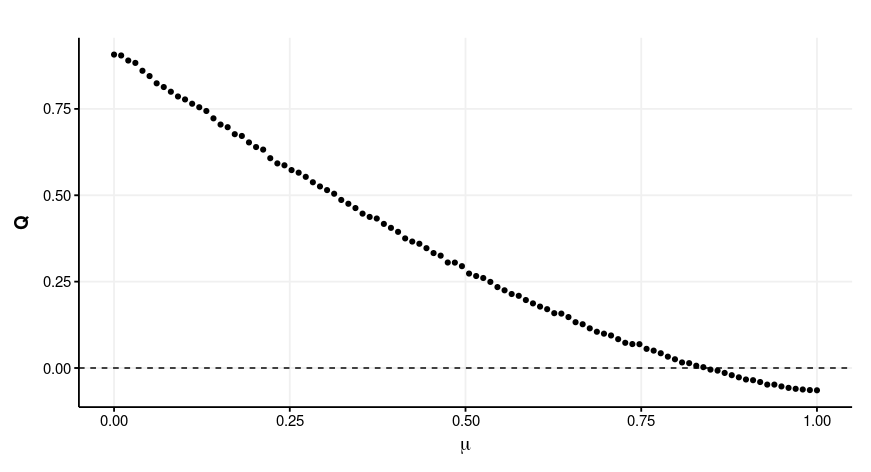
\includegraphics[width=0.9\textwidth]{images/chapter_community_detection/ggplot2/LFR/Rplot_muandq_theme.png}
    \caption[Modularity and $\mu$ for LFR benchmark]{Plot of modularity with parameter $mu$ in LFR benchmark. Using LFR 3457 40617 benchmark}
    \tiny Plot \url{source('~/RProjects/fortunato/R/plot/new_plot_qandmu.R')}
    \tiny Calculations \url{/home/grant/Projects_/Python/src/Qandmu.ipynb}
    \label{fig:modularity_and_mu}
\end{figure}

% \subsubsection{Testing}
% Infomap and louvain do very well on lfr but spectral not so well. Infomap does perfectly with nmi but poorly with real world network. 
% settings = \url{g2= nx.generators.LFR_benchmark_graph(n=graph_n, tau1=3, tau2=1.1, mu=0.1, average_degree=10, max_degree=50, min_community=10,max_community=50, seed=1)}

% Set seed 1 See table~\ref{tab:benchmark LFR size 1000}

% \begin{table}[h]
%     \centering
%     \begin{tabular}{ll}
%     \toprule
%      Method    & NMI  \\
%      \midrule
%     Louvain     & 0.970\\
%     Infomap     & 1\\
%     Spectral & 0.949\\
%     Greedy & 0.873\\
%     Leading eigenvector & 0.620\\
%     Label propogation & 0.997\\
%     Out walk trap & 0.995\\
%     \bottomrule
%     \end{tabular}
%     \caption{Benchmark LFR size 1000. Generated using networkx for python}
%     \label{tab:benchmark LFR size 1000}
% \end{table}
% % Louvain =  0.9705355030878491

% % Info = 1 

% % Spec = 0.9486340326647721

% % Greedy = 0.8736469937608322

% % Leading eigenvector method igraph = 0.6202572106629003

% % Label propogation = 0.9966685735031502

% % Out walk trap = 0.9952730301593156

% its all the small or zero groups that give good nmi as the number of correctly misclassified is right so long as vertices a and b if in different groups are in different groups 
\subsubsection{Methods}
\label{sec:LFT methods}
The LFR benchmark networks were generated using the Python package NetworkX (version 2.4)\cite{hagberg2008exploring}. In addition to the power law exponent of the degree distribution either the minimum/maximum degree or average degree can be provided as arguments to generate the desired degree distribution\footnote{Remove: the (problem is exponential does not hold from x min equal to 1 gamma is 1.38 and 5 is 1.81, 2.51 using clauset)}.

Setting the minimum and maximum degree using the values of the PSP and the degree exponent of 2.51 produces a network with  roughly equal vertices and edges (V:3457, E:4736), a mean degree of 2.74, and maximum degree 119 (degree assortativity -0.09, global transitivity 0.012). This is clearly a poor model for the PSP\footnote{bring out that this is one of the things you find out ie that it is problematic but that the reason lfr is not great for transitivity is when you set the minimum degree but the other side is that if you set the mean degree you get lots of nodes less than 7}.

If instead, using the same degree exponent, one sets the mean degree parameter equal to the PSP mean (rather than setting minimum or maximum degree) the network is much more like the PSP although there are no nodes of degree less than seven (these make up 1,445 vertices of the PSP graph) \footnote{(Degree 1:304, Degree 2:293, 3:248 4:245 5:188 6:167)}equivalent to 41.7\% of the vertices.  This may be because the power law distribution does not hold in the low degree region of the degree distribution. The LFR benchmark graph thus generated has 3457 nodes and 40617 edges.
Modularity was 0.431 for ground truth community allocations($\mu$=0.375). The graph is available in .gml format at \url{git@github.com:14760/ipynotebooks_phd.git}

The Louvain and Infomap algorithms perform have been shown to perform well on the LFR benchmark\cite{lancichinetti2008benchmark},\cite{lancichinetti2009community} although the networks produced using the default network settings in\cite{lancichinetti2008benchmark} are quite dissimilar to the the PSP.
 A spectral algorithm was tested, the leading eigenvector method\cite{newman2006finding}, without fine tuning step\cite{lancichinetti2008benchmark}. The LFR benchmark has limitations, in addition to the difficulty in generated particular networks it is known to produce similar sized communities which differ from  real world networks\cite{orman2013towards},\cite{aldecoa2013exploring}. 

Networks generated using the LFR benchmark are reported to have low transitivity and zero degree correlation in common with many other generative models and so do not completely capture the structure of complex networks \cite{orman2013towards},\cite{orman2009comparison}. However using the `PSP like' LFR network it is interesting to note the degree assortativity is -0.16  (PSP r=-0.18) table~\ref{Table:DegreeAssortativityNewman}) and the transitivity $C$=0.0415  (PSP=0.067section~\ref{sec:results_global_clustering_coefficient} )and  $C_{WS}$ =0.0810\footnote{\tiny Code to generate LFR benchmark at\url{/home/grant/Projects_/Python/venvs/Create_LFR_similar_to_PSP.ipynb}}.

Given some of the limitations of the LFR benchmark, I have also used the performance of algorithms on the PSP, as measured by modularity and plausibility of group size, to determine the most appropriate algorithms to use. 


\paragraph{Normalised mutual information}
Normalised mutual information (NMI) is a measure of the amount of information obtained about a partition of the network by knowing another partition. It has been used as a measure of the quality of partitions of a network\cite{danon2005comparing} and lies in the range 0-1. The algorithms were assessed on the LFR benchmark by comparing the detected communities to the ground truth partition using Normalised Mutual Information with igraph. The mutual information, adjusted for the expected value of the mutual information\cite{vinh2010information}, was calculated using scikit-learn\cite{abraham2014machine}. Normalised mutual information was also used to compare the similarity of the communities discovered in the PSP but here the communities found by different algorithms are compared against one another rather than ground truth. 




% \textcolor{red}{This is bollocks}For a degree structure similar to the PSP it proved impossible to generate a community structure with a power exponent greater than 1.156 in the network x implementation of the LFR benchmarks using 1000 iterations (parameters - average degree 27, min\_community=20) .  Increasing minimum community size to 50 allowed a maximum $\beta$ of 1.6.\textcolor{red}{end}











% \subsubsection{Testing}
% Infomap and louvain do very well on lfr but spectral not so well. Infomap does perfectly with nmi but poorly with real world network. 
% settings = \url{g2= nx.generators.LFR_benchmark_graph(n=graph_n, tau1=3, tau2=1.1, mu=0.1, average_degree=10, max_degree=50, min_community=10,max_community=50, seed=1)}

% Set seed 1 See table~\ref{tab:benchmark LFR size 1000}

% \begin{table}[h]
%     \centering
%     \begin{tabular}{ll}
%     \toprule
%      Method    & NMI  \\
%      \midrule
%     Louvain     & 0.970\\
%     Infomap     & 1\\
%     Spectral & 0.949\\
%     Greedy & 0.873\\
%     Leading eigenvector & 0.620\\
%     Label propogation & 0.997\\
%     Out walk trap & 0.995\\
%     \bottomrule
%     \end{tabular}
%     \caption{Benchmark LFR size 1000. Generated using networkx for python}
%     \label{tab:benchmark LFR size 1000}
% \end{table}
% % Louvain =  0.9705355030878491

% % Info = 1 

% % Spec = 0.9486340326647721

% % Greedy = 0.8736469937608322

% % Leading eigenvector method igraph = 0.6202572106629003

% % Label propogation = 0.9966685735031502

% % Out walk trap = 0.9952730301593156

% its all the small or zero groups that give good nmi as the number of correctly misclassified is right so long as vertices a and b if in different groups are in different groups 


\subsection{LFR Performance}

The performance of the igraph community detection algorithms, Markov Cluster algorithm, the spectral clustering algorithm and the nested stochastic block model on the LFR (PSP like) benchmark graph (see above) are shown in table~\ref{tab:Modularity, NMI and adjusted NMI on the LFR Benchmark PSPlike}. A sizeable difference is seen between the NMI and Adjusted NMI particularly for the Markov Clustering partition supporting the utility of this measure\cite{vinh2010information}. The Markov Cluster algorithm method (adjusted NMI=0.127), leading eigenvector method (adjusted NMI=0.134) perform poorly and the fast greedy (adjusted NMI=0.457) algorithm does poorly despite good performance on modularity ($Q=$0.368). The stochastic block model performs better when it has more groups rather than when it is nested (SBM level 0 adj NMI 0.846 Communities $n$=52 see also table~\ref{tab:Group sizes compared with ground truth LFR 3457 PSP like benchmark}). The unnested stochastic block model was a has a low modularity partition (Q=0.175) despite good performance on the NMI the converse of fast greedy. 

Table~\ref{tab:Group sizes compared with ground truth LFR 3457 PSP like benchmark} shows the distribution of community sizes found on the LFR benchmark network. The Markov Cluster algorithm generates a large number of communities ($n=1621$). We expect divisive algorithms to give rise to some small communities (as agglomerative ones do large ones) but the proportion of nodes in communities that are larger than the recommended minimum community size for GSEA is only 42.4\% compared with 97.98\% for the spectral CDM algorithm and 99.65\% for label propagation (table~\ref{tab:Group sizes compared with ground truth LFR 3457 PSP like benchmark filtered for size less than 15}). The fast greedy algorithm creates a small number of communities ($n=8$) with a high median degree (432.1 vs ground truth(gt) 96.3) as does the leading eigenvector (LEC) method. Walk trap, infomap, and label propagation median group size is close to that of ground truth. The spectral algorithm matches median community size well once the small number of communities smaller than GSEA default have been removed(see figure~\ref{fig:boxplot group size lfr clustering methods}). The comparison of community sizes to ground truth with small groups (<15 members) removed is shown in figure~\ref{tab:Group sizes compared with ground truth LFR 3457 PSP like benchmark filtered for size less than 15}.


\paragraph{PSP} Examination of the performance of the community detection algorithms on the PSP network shows that the maximum modularity is found in the Louvain algorithm and SpinglassG1 ($\gamma=1$) (q=0.34). 
Some of the clusters have slightly higher modularity than the ground truth\footnote{\url{/home/grant/Projects_/Python/venvs/Create_LFR_similar_to_PSP_Copy_inc_SG_for_table.ipynb} on redmachine}The Geodesic edge betweenness in addition to its slow running time performs most poorly (0.10). Table~\ref{tab:modularity and group sizes PSP xtable} shows that the Geodesic algorithm and walktrap have an improbably large number of communities (2,566 and 562). The infomap algorithm has a modularity of $Q=0.28$ but has 171 communities with a maximum size of 1,228. The algorithms that perform adequately well on all measures are the spinglass algorithms, Louvain and spectral. As figure~\ref{fig:boxplot group size lfr clustering methods} shows the spectral algorithm matches the ground truth community sizes reasonably well considering that the LFR using average degree has a minimum community size of 16 and spectral clustering has 34 communities of size less than fifteen however excluding these results in a loss of only 2.02\% of the genes (compared with 47.56 for MCL table~\ref{tab:Group sizes compared with ground truth LFR 3457 PSP like benchmark}). A community equal to one could be considered in a way analogous to not assigning a community number to it. 24 entries equal to 1. \footnote{Code at \url{source('~/RProjects/python_benchmarks/R/make_table_lfr_benchmark_group_sizes.R')}}
\footnote{Python code to generate the LFR model and test it is at \url{/home/grant/Projects_/Python/venvs/Create_LFR_similar_to_PSP.ipynb} this is on red bionic beaver machine}


These results agree with the general trend of the literature\cite{yang2016comparative},\cite{newman2018networks},\cite{fortunato2016community}. I chose to use the spectral method as it had performed well across all measures, has good performance and differential enrichment previously on PSP like networks\cite{mclean2016improved} and we had expertise in the implementation of the algorithm in our group. The Louvain algorithm was very attractive with a superior modularity to the spectral algorithm on the PSP (0.34 vs 0.30), but the communities were larger than one would prefer with Louvain (double median in LFR, median 190 PSP) and therefore slightly less suited to GSA (see section~XX for large groups in GWA analysis). The number of  potential parameters mitigated against the choice of spinglass as the choice of parameters would complicate study design. In addition with $\gamma=5$ the groups seemed particularly large and similar in size and all were large compared to ground truth on LFR\footnote{from the point of view of study design large being worse than numerous small which can be excluded}.








% Using a 3457 LFR graph (18061 edges) the ground truth is of 143 communities
\todo{look at commented out bit here}
% Community size however varied with different methods


% \begin{table}[]
%     \centering
%     \begin{tabular}{lll}
%     \toprule
%         Method & n communites & NMI  \\
%         \midrule
%         Ground truth  & 143 & 1 \\
%         Louvain & 74 & 0.934 \\
%         Infomap & 143 & 0.9996 \\
%         igraph eigenvector & 60 & 0.599\\gamma1
%         Label propagation & 147 & 0.999\\
%         Walk trap & 139 & 0.996\\
%         Spectral & 129 & 0.950\\
%         \bottomrule
%     \end{tabular}
%     \caption{Performance of algorithms against groun truth for 3457 node 18061 generated LFR benchmark network}
%     \label{tab:benchmark Performance of algorithms against groun truth for 3457 node 18061 generated LFR benchmark network}
% \end{table}
% %Length louvain = 74

% %  Length info = 143
 
% %  Length greedy = 61
 
% %  Length eig = 60
 
% %  Length label = 147
 
% %  Length walk trap = 139
 
% %  Comparison of louvain and ground truth method nmi result 0.9342619557388658
 
% % Comparison of infomap and ground truth method nmi result 0.9995553221817195

% % Comparison of greedy and ground truth method nmi result 0.886167941390111

% % Comparison of igraph eigenvector and ground truth method nmi result 0.5990794237801158

% % Comparison of label propagation and ground truth method nmi result 0.9992978887550072

% % Comparison of walk trap and ground truth method nmi result 0.9966928932427445

% % Spectral nmi = 0.950168278988933

% % Spectral communities 129

% Comparison of louvain and ground truth method split-join result 1088.0
% Comparison of infomap and ground truth method split-join result 4.0
% Comparison of greedy and ground truth method split-join result 1607.0
% Comparison of igraph eigenvector and ground truth method split-join result 3397.0
% Comparison of label propagation and ground truth method split-join result 52.0
% Comparison of walk trap and ground truth method split-join result 51.0

% This is a distance metric that is asymmetrical

% Spectral 573


% Comparison of louvain and ground truth method adjusted\_rand result 0.7240323254646376
% Comparison of infomap and ground truth method adjusted\_rand result 0.9992769735118784
% Comparison of greedy and ground truth method adjusted\_rand result 0.5230033392550409
% Comparison of igraph eigenvector and ground truth method adjusted\_rand result 0.1556290274596547
% Comparison of label propagation and ground truth method adjusted\_rand result 0.9951401364385163
% Comparison of walk trap and ground truth method adjusted\_rand result 0.9877048741950667


% Spectral adjusted rand
% 0.8562028042791093

% Variational information of melia (distance identity is 0)

% Comparison of louvain and ground truth method vi result 0.599081269091533
% Comparison of infomap and ground truth method vi result 0.004317734259799977
% Comparison of greedy and ground truth method vi result 1.0019588805230972
% Comparison of igraph eigenvector and ground truth method vi result 3.3729468833994076
% Comparison of label propagation and ground truth method vi result 0.004766377185209336
% Comparison of walk trap and ground truth method vi result 0.03202630730712208

% Spectral 
% 0.476519814388233





% latex table generated in R 3.6.3 by xtable 1.8-4 package
% Wed Apr 28 18:23:23 2021
\begin{table}[ht]
\centering
\setlength{\extrarowheight}{2pt}
\begin{tabular}{llll}
  \toprule
Method & Modularity & NMI & Adjusted NMI \\ 
  \midrule
Ground truth & 0.431 & 1.000 & 1.000 \\ 
  Infomap & 0.432 & 0.974 & 0.971 \\ 
  Spinglass gamma2 & 0.429 & 0.914 & 0.887 \\ 
  Spinglass gamma1 & 0.433 & 0.931 & 0.882 \\ 
  Louvain & 0.432 & 0.913 & 0.870 \\
  Walktrap & 0.423 & 0.893 & 0.870 \\ 
  sbm level 0 & 0.174 & 0.911 & 0.846 \\ 
  Label prop & 0.416 & 0.835 & 0.800 \\ 
  Spinglass gamma5 & 0.379 & 0.810 & 0.796 \\ 
  Spectral & 0.392 & 0.782 & 0.762 \\ 
  sbm level 1 & 0.374 & 0.751 & 0.607 \\ 
  Fast Greedy & 0.368 & 0.564 & 0.457 \\ 
  sbm level 2 & 0.259 & 0.468 & 0.307 \\ 
  Markov clustering & 0.127 & 0.653 & 0.295 \\ 
  LEC & 0.187 & 0.190 & 0.134 \\ 
   \bottomrule
\end{tabular}
\caption{Modularity, NMI and adjusted NMI on the LFR Benchmark PSP like} 
\tiny\url{source('~/RProjects/python_benchmarks/R/format_LFR_Q.R')}
\tiny\url{/home/grant/Projects_/Python/src/get_modularity_lfr.ipynb}
\label{tab:Modularity, NMI and adjusted NMI on the LFR Benchmark PSPlike}
\end{table}
% latex table generated in R 3.6.3 by xtable 1.8-4 package
% Sat Jul 11 16:22:32 2020

% latex table generated in R 3.6.3 by xtable 1.8-4 package
% Sat Jul 11 16:23:53 2020
% \begin{table}[ht]
% \centering
% \begin{tabular}{lccccccc}
%   \toprule
%   community detection method & n & Minimum & 1st Qua. & Median & Mean & 3rd Quartile & Max. \\ 
%   \midrulegamma1
%   Ground truth & 35should be 36 index from 0 & 16 & 37.8 & 57 & 96.0 & 107.8 & 558 \\ 
%   Louvain & 23 & 18 & 60.2 & 110 & 144.0 & 204.2 & 573 \\ 
%   Infomap & 38 & 2 & 29.0 & 50 & 88.6 & 96.5 & 568 \\ 
%   Greedy  & 7 & 205 & 371.0 & 407 & 432.1 & 502.2 & 633 \\ 
%   Leading eigenvector & 4 & 287 & 448.0 & 593 & 691.4 & 905.0 & 1224 \\ 
%   \textbf{Label propagation }& 0 & 3457 & 3457.0 & 3457 & 3457.0 & 3457.0 & 3457 \\ 
%   Walktrap & 32 & 15 & 35.0 & 55 & 104.8 & 139.0 & 633 \\ 
%   Spectral & 65 & 1 & 1.0 & 8 & 52.4 & 68.5 & 518 \\ 
%   SG1&\\
%   SG2&\\
%   SG5&\\
%   Markov&\\
%   SBM&\\
%   \bottomrule
% \end{tabular}
% \caption{Group size on lfr3457\url{g1=nx.generators.LFR_benchmark_graph(n=graph_n,tau1= 2.51,tau2 = 1.5,mu= 0.375,average_degree=17,max_degree= 405, min_community= 15,max_community= 1000,seed=seed)}. n= number of communities, 1st Qua = 1st quartile of community group size, 3rd qua= 3rd quartile, Max. = maximum group size } 
% \label{tab:Group size on lfr 3457 }
% \end{table}

% latex table generated in R 3.6.3 by xtable 1.8-4 package
% Wed Apr 21 17:34:51 2021
\begin{table}[ht]
\centering
\setlength{\extrarowheight}{2pt}
\begin{tabular}{llllllll}
  \toprule
 & n & Min. & 1Q & Median & Mean & 3Q & Max. \\ 
  \midrule
Ground truth & 36 & 16 & 37.75 & 57.0 & 96.0 & 107.75 & 558 \\ 
Markov Cluster & 1621 & 1 & 1.00 & 1.0 & 2.1 & 1.00 & 148 \\ 
Spectral & 66 & 1 & 1.00 & 8.5 & 52.4 & 68.50 & 518 \\ 
 Louvain & 24 & 18 & 60.25 & 110.0 & 144.0 & 204.25 & 573 \\ 
 Infomap & 39 & 2 & 29.00 & 50.0 & 88.6 & 96.50 & 568 \\ 
 Label Prop. & 26 & 12 & 40.25 & 64.5 & 133.0 & 177.25 & 793 \\ 
 Fast greedy & 8 & 205 & 371.00 & 407.0 & 432.1 & 502.25 & 633 \\ 
 Spinglass gamma1 & 24 & 18 & 79.50 & 115.0 & 144.0 & 180.50 & 564 \\ 
 Spinglass gamma2 & 25 & 60 & 76.00 & 99.0 & 138.3 & 176.00 & 481 \\ 
 Spinglass gamma5 & 25 & 98 & 113.00 & 129.0 & 138.3 & 156.00 & 208 \\ 
 SBM 0 & 52 & 12 & 24.00 & 40.5 & 66.5 & 72.00 & 377 \\ 
 SBM 1 & 10 & 83 & 132.25 & 216.5 & 345.7 & 414.50 & 991 \\ 
 SBM 2 & 3 & 629 & 849.50 & 1070.0 & 1152.3 & 1414.00 & 1758 \\ 
 LEC (Leading eigenvector) & 5 & 287 & 448.00 & 593.0 & 691.4 & 905.00 & 1224 \\ 
 Walktrap & 33 & 15 & 35.00 & 55.0 & 104.8 & 139.00 & 633 \\ 
   \bottomrule
\end{tabular}
\caption{Group sizes compared with ground truth LFR 3457 `PSP like' benchmark. SBM stochastic block model, number refers to level of nesting - level zero is nested in one and in turn nested in two which therefore has the smallest $n=3$ number of communities. 1Q and 3Q first and third quartile. $n$ number of communities} 
\tiny\url{source('~/RProjects/python_benchmarks/R/make_table_gt_lfr_3457.R', echo=TRUE)}
\label{tab:Group sizes compared with ground truth LFR 3457 PSP like benchmark}
\end{table}






% latex table generated in R 3.6.3 by xtable 1.8-4 package
% Sun Apr 25 17:46:08 2021
\begin{table}[ht]
\centering
\begin{adjustbox}{width=\textwidth}

\setlength{\extrarowheight}{2pt}
\begin{tabular}{rrrrrrrrrrr}
  \toprule
 & Min & 1Q & Median & Mean & 3Q & Max & n & coverage & n comm &  n max comm \\ 
  \midrule
gt & 16 & 37.75 & 57 & 96.03 & 107.75 & 558 & 3457 & 100.00 & 36 & 36 \\ 
  mcl & 18 & 25.00 & 39 & 54.33 & 71.00 & 148 & 1467 & 42.44 & 27 & 1621 \\ 
  spe & 17 & 40.25 & 72 & 105.84 & 121.25 & 518 & 3387 & 97.98 & 32 & 66 \\ 
  louvain & 18 & 60.25 & 110 & 144.04 & 204.25 & 573 & 3457 & 100.00 & 24 & 24 \\ 
  info & 15 & 32.75 & 56 & 95.86 & 111.25 & 568 & 3451 & 99.83 & 36 & 39 \\ 
  label\_prop & 18 & 44.00 & 67 & 137.80 & 190.00 & 793 & 3445 & 99.65 & 25 & 26 \\ 
  fg & 205 & 371.00 & 407 & 432.12 & 502.25 & 633 & 3457 & 100.00 & 8 & 8 \\ 
  SG1 & 18 & 79.50 & 115 & 144.04 & 180.50 & 564 & 3457 & 100.00 & 24 & 24 \\ 
  SG2 & 60 & 76.00 & 99 & 138.28 & 176.00 & 481 & 3457 & 100.00 & 25 & 25 \\ 
  SG5 & 98 & 113.00 & 129 & 138.28 & 156.00 & 208 & 3457 & 100.00 & 25 & 25 \\ 
  sbm0 & 15 & 25.00 & 41 & 67.55 & 75.00 & 377 & 3445 & 99.65 & 51 & 52 \\ 
  sbm1 & 83 & 132.25 & 216 & 345.70 & 414.50 & 991 & 3457 & 100.00 & 10 & 10 \\ 
  sbm2 & 629 & 849.50 & 1070 & 1152.33 & 1414.00 & 1758 & 3457 & 100.00 & 3 & 3 \\ 
  lec & 287 & 448.00 & 593 & 691.40 & 905.00 & 1224 & 3457 & 100.00 & 5 & 5 \\ 
  wt & 15 & 35.00 & 55 & 104.76 & 139.00 & 633 & 3457 & 100.00 & 33 & 33 \\ 
   \bottomrule
\end{tabular}
\end{adjustbox}
\caption{Group sizes compared with ground truth LFR 3457 PSP like benchmark filtered for size less than 15} 
\tiny\url{source('~/RProjects/python_benchmarks/R/make_table_gt_lfr_3457_sizefilter.R')}
\label{tab:Group sizes compared with ground truth LFR 3457 PSP like benchmark filtered for size less than 15}
\end{table}




% latex table generated in R 3.6.3 by xtable 1.8-4 package
% Sun Apr 25 17:53:40 2021
\begin{table}[ht]
\centering
\begin{adjustbox}{width=\textwidth}

\setlength{\extrarowheight}{2pt}
\begin{tabular}{rrrrrrrrrrr}
  \toprule
  & Min & 1Q & Median & Mean & 3Q & Max & n & coverage & n comm &  n max comm \\ 
  \midrule
  gt & 16 & 37.75 & 57 & 96.03 & 107.75 & 558 & 3457 & 100 & 36 & 36 \\ 
mcl & 18 & 25.00 & 39 & 54.33 & 71.00 & 148 & 1467 & 42.44 & 27 & 1621 \\ 
  spe & 17 & 40.25 & 72 & 105.84 & 121.25 & 518 & 3387 & 97.98 & 32 & 66 \\ 
  info & 15 & 32.75 & 56 & 95.86 & 111.25 & 568 & 3451 & 99.83 & 36 & 39 \\ 
  label\_prop & 18 & 44.00 & 67 & 137.80 & 190.00 & 793 & 3445 & 99.65 & 25 & 26 \\ 
  sbm0 & 15 & 25.00 & 41 & 67.55 & 75.00 & 377 & 3445 & 99.65 & 51 & 52 \\ 
   \bottomrule
\end{tabular}
\end{adjustbox}
\caption{Group sizes compared with ground truth LFR 3457 PSP like benchmark filtered for size less than 15} 
\tiny\url{source('~/RProjects/python_benchmarks/R/make_table_gt_lfr_3457_sizefilter2.R')}
\label{tab:Group sizes compared with ground truth LFR 3457 PSP like benchmark filtered for size less than 15 filter}
\end{table}






  \begin{figure}
      \centering
      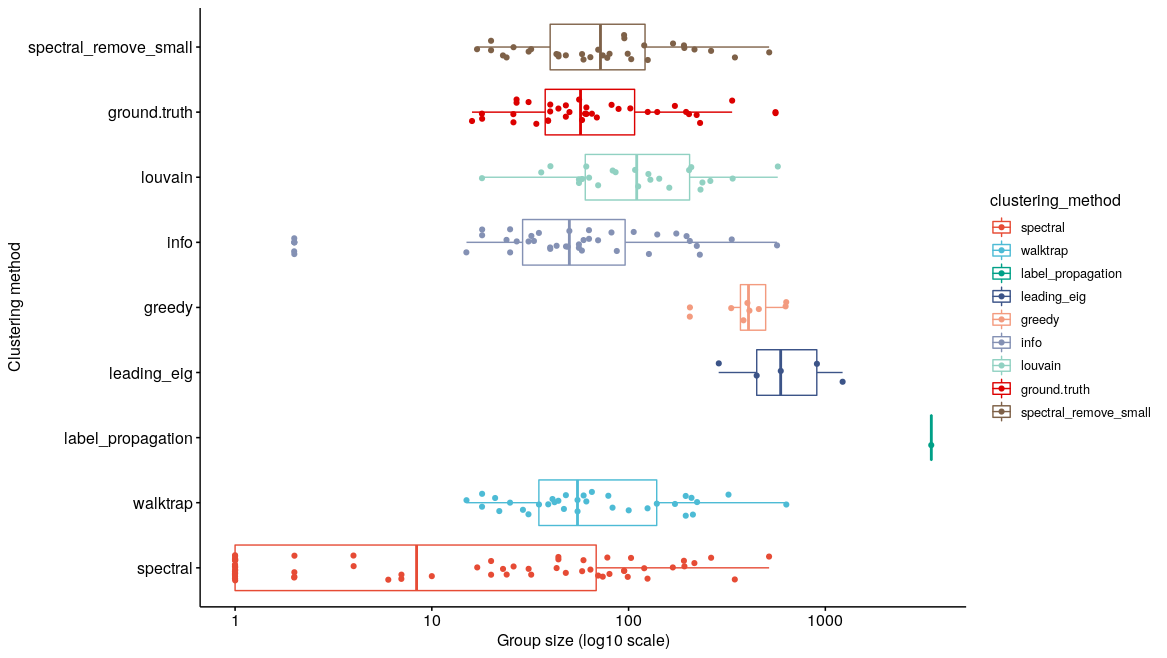
\includegraphics[width=\textwidth]{images/Rplot_draft_plot_boxplot_group_sizes_lfr.png}
      \caption{Boxplot of sizes of communities detected for various clustering methods on a 3457 node 40617 edge benchmark LFR benchmark graph. Code to generate at \url{source('~/RProjects/python_benchmarks/R/plot_boxplot_group_sizes_lfr.R')}}
      \label{fig:boxplot group size lfr clustering methods}
  \end{figure}
 
 




\subsection{Optimal community size}
\label{sec:optimal community size}
Real world communities tend to show a core and whisker structure. The whiskers tend to be good communities but larger groups discovered by clustering algorithms tend to belong to the core or represent the core and have lower conductance and hence are less cohesive as groups. We can see this pattern of size distribution in the communities discovered in the PSP for particular algorithms \todo{cross ref}. The spectral clustering algorithm and Louvain algorithm produce communities of less disparate size although the Louvain clusters are large. \todo{graph of conductance versus community sizes}

Approximately 80\% of nodes are in the core \todo{check ref that is from zhukov}
\todo{what does core represent if we are not including core chapter}

\cite{leskovec2010empirical}

Median conductance Spectral size 15 0.7188\footnote{\url{source('~/RProjects/fortunato/R/calculate_fortunato_measures_name_input.R')}}

Median conductance Louvain 0.58 


\section{Results benchmark}

\subsubsection{Infomap Results benchmark}
The infomap algorithm is popular, is fast, and has performed well on standardised benchmarks such as the LFR benchmark \todo{add cross reference}\cite{lancichinetti2008benchmark}, \cite{newman2018networks}. A recent comparison of algorithms implemented in igraph\cite{yang2015defining} showed its performance was poorer in networks with higher noise on the LFR benchmark.  \todo{check the lanchichinetti refs there should maybe also be the 2009 one}. Algorithms that perform well on the LFR benchmark can give rise to communities of unrealistic sizes with on the PSP network and it can be difficult to reproduce exactly the degree structure of the PSP network given the parameters of the LFR benchmark. The infomap method has been seen to perform poorly with more noise \cite{yang2016comparative}, benchmarking it against the stochastic block model as the community structure approaches the  limits of resolution there is a dramatic deterioration in performance. It provides a relatively low modularity for the partition and finds a large number of small groups and one very large one (see table~\ref{tab:modularity and group sizes xtable}). 



\section{Performance on PSP graph}
\label{sec:Performance on PSP graph}
The group sizes and modularity of the above algorithms on the PSP graph are shown in table~\ref{tab:modularity and group sizes xtable}. Figure~\ref{fig:community_sizes_no_size_filter} shows a boxplot of community size for different clustering algorithms.  Spin glass with gamma = 2 is close to the `good' level of 100 members. Spectral is a little low and the louvain algorithm high although all three have acceptable modularity (table~\ref{tab:modularity and group sizes xtable}. Figure~\ref{fig:community_sizes_size_filter_added} shows the effect of filtering out small groups that might have biased assessments using GSA\cite{de2016statistical} using fifteen the default lower bound for GSEA. Only 2.5\% of genes are excluded from the spectral clustering method but the median is much closer to 100 now and trhe interquartile range much narrower. 


The walk trap algorithm and geodesic produce many communities and have suboptimal modulairty. Mean community size is only 6.2 for walktrap and 1.3 for geodesic but both contain large groups 496 in the case of geodesic, 760 in the case of walktrap. The igraph implementation of spectral clustering (LEC) divides the network into three groups all larger than 1000 nodes. Infomap shows a very wide size range and a large number of communities (171) its largest community is 1228 in size (35.5\% of the PSP). 916 nodes belonged to 134 groups less than size 15. Only 36 groups were greater than or equal to 15 and smaller than the largest group (1313 genes) table~\ref{tab:modularity and group sizes PSP xtable}. The second largest group has 130 members.  134 of the infomap communities are less than 15 in size, 103 less than 10, and 39 less than 5. 15.9\% of the network is made up of groups of size less than 10. The promising algorithms are therefore louvain, spectral, and spinglass 2 and 5. The spinglass algorithms have the problem of additional parameters and preference would therefore be louvain or spectral. Both (louvain and spectral) have similar community size to ground truth in figure~\ref{fig:boxplot group size lfr clustering methods}. 

The Louvain algorithm is agglomerative and tends towards larger groups and the number of communities ($n=14$) seems intuitively a little low. The spectral is divisive and produces a number of small groups but the ones that are problematically small make up a small amount of the graph. Although there is little to chose between the two the spectral `looked better', had performed well on a pilot study (not shown) and there is also a warning against large groups in \cite{de2016statistical}.



Table~\ref{tab:Group size of clusters excluding gene sets size less than 15} shows a summary of the group sizes. With very small groups excluded mean and median group size are almost doble for louvain than spectral. 
\paragraph{PSP}





  The actual allocation does not matter as much for the NMI and other metrics as getting those not in the same group not in the same group but does matter for GSA. Similarly discarding those with size less than 15 is not a problem with GSA.\footnote{Code for fortunato of LFR benchmark \url{source('~/RProjects/fortunato/R/calculate_fortunato_measures_name_input_and_graph.R')}},\footnote{Code for modularity and mu \url{/home/grant/Projects_/Python/venvs/src/effect_of_mu.py} NB this is on red machine beaver}

% latex table generated in R 3.6.3 by xtable 1.8-4 package
% Fri Apr  9 18:20:38 2021
\begin{table}[ht]
\centering
\begin{tabular}{lrrrrrrrr}
  \toprule
clustering\_method & min & mean & median & IQR & max & n & tot & coverage \\ 
  \midrule
lec & 1111 & 1152.3 & 1134 & 50.5 & 1212 & 3 & 3457 & 1.000 \\ 
  wt & 16 & 106.6 & 26 & 60.5 & 760 & 24 & 2559 & 0.740 \\ 
  fc & 34 & 426.8 & 134 & 896.2 & 1095 & 8 & 3414 & 0.988 \\ 
  sgG1 & 30 & 311.1 & 236 & 486.0 & 672 & 11 & 3422 & 0.990 \\ 
  sgG2 & 15 & 95.7 & 87 & 79.0 & 269 & 36 & 3444 & 0.996 \\ 
  sgG5 & 15 & 33.8 & 29 & 18.5 & 98 & 95 & 3215 & 0.930 \\ 
  Geodesic & 15 & 98.6 & 21 & 44.0 & 496 & 7 & 690 & 0.200 \\ 
  Spectral & 20 & 96.3 & 72 & 99.0 & 405 & 35 & 3369 & 0.975 \\ 
  louvain & 21 & 246.9 & 190 & 224.5 & 539 & 14 & 3457 & 1.000 \\ 
  infomap & 15 & 68.7 & 27 & 32.0 & 1228 & 37 & 2541 & 0.735 \\ 
   \bottomrule
\end{tabular}
\caption{Group size of clusters excluding gene sets size less than 15 PSP} 
\tiny\url{source('~/RProjects/fortunato/R/summary_table/calculate_PSP_Group_sizes_boxplot_add_sizefilter_summary_table.R')}
\label{tab:Group size of clusters excluding gene sets size less than 15}
\end{table}



\begin{table}[ht]
\centering

\begin{tabular}{rrrrrrr}
  \toprule
method & Q & n & min & max & median & mean \\ 
  \midrule
lec & 0.25 & 3 & 1111 & 1212 & 1134.0 & 1152.3 \\ 
  walktrap & 0.26 & 562 & 1 & 760 & 1.0 & 6.2 \\ 
  louvain & 0.34 & 14 & 21 & 539 & 190.5 & 246.9 \\ 
  Spinglass gamma1 & 0.34 & 18 & 2 & 672 & 35.0 & 192.1 \\ 
  Spinglass gamma2 & 0.33 & 38 & 5 & 269 & 85.5 & 91.0 \\ 
  Spinglass gamma5 & 0.26 & 118 & 4 & 98 & 26.0 & 29.3 \\ 
  infomap & 0.28 & 171 & 2 & 1228 & 8.0 & 20.2 \\ 
  spectral & 0.30 & 65 & 1 & 405 & 27.0 & 53.2 \\ 
  geodesic & 0.10 & 2566 & 1 & 496 & 1.0 & 1.3 \\ 
  fast greedy (fc) & 0.31 & 19 & 2 & 1010 & 8 & 181.9 \\
   \bottomrule
\end{tabular}
\caption[[Modularity and group size for different clustering modalities PSP]{modularity and group sizes PSP. Louvain, spinglass and spectral have the best modularity. The fast greedy algorithm has a good modularity but contains an implausibly large group $n=1010$} 
\label{tab:modularity and group sizes PSP xtable}
\end{table}

\begin{figure}
    \centering
    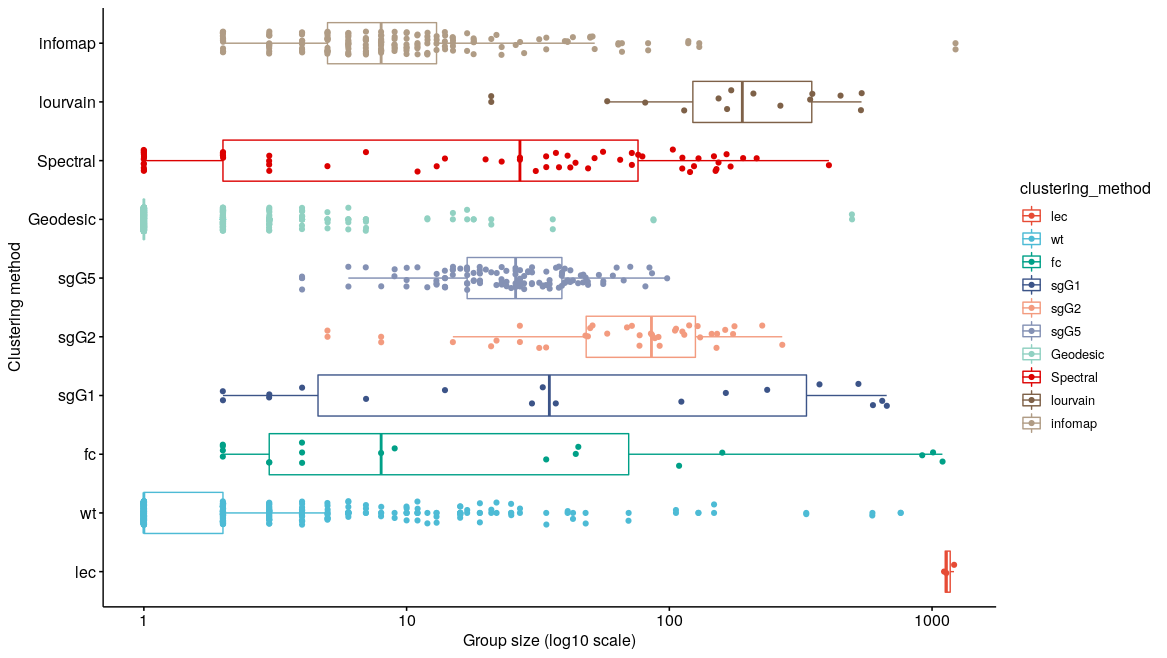
\includegraphics[width=0.9\textwidth]{images/Rplot_boxplot_group_sizes_different_methods_size_1_or_greater.png}
    \caption{Boxplot of  
    the sizes of communities detected in the post synaptic proteome network using different community detection methods. The boxplot shows all communities and is not filtered by community size. Scale of response (group size) scaled by log10.}
    \tiny\url{source('~/RProjects/fortunato/R/calculate_PSP_Group_sizes_boxplot.R')}
    \label{fig:community_sizes_no_size_filter}
\end{figure}


\begin{figure}
    \centering
    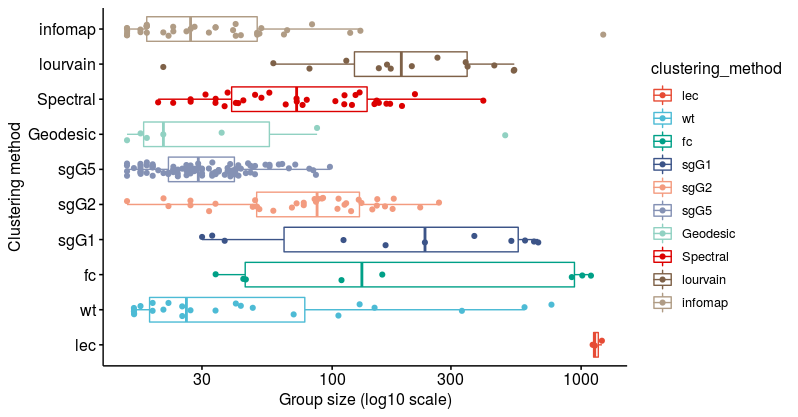
\includegraphics[width=0.9\textwidth]{images/chapter_community_detection/ggplot2/community_sizes_PSP/Rplot_PSP_groupsizes_clustering_size_filter_fifteen.png}
    \caption{Boxplot of  
    the sizes of communities detected in the post synaptic proteome network using different community detection methods. The boxplot shows all communities and is filtered by community size. Only communities greater than or equal to fifteen members. Scale of response (group size) scaled by log10. Spectral clustering with small groups remmoved has a median close to the ideal of size 100}
    \tiny\url{source('~/RProjects/fortunato/R/calculate_PSP_Group_sizes_boxplot_add_sizefilter.R')}
    \label{fig:community_sizes_size_filter_added}
\end{figure}


erable variation in group size. Some methods give rise to very extreme group size values with a large number of size 1 groups or a small number of very large groups. There is some reason to believe (LFR) that in empirical networks there is a power law distribution of group size however there are some features we would like in the community detection algorithm. For the reasons in section (GSA) we would like communities of a reasonable (15 or more for example) size to avoid the signal being dominated by a small number of genes or the sample being too Check that the volume is equal to 2 x the edge count  TRUE 
small to represent a group. We would however like that the number of genes we exclude on size criteria (either too large or too small) should not be a disproportionately large part of the PSP. In this way we also want to avoid very large groups. There is evidence that groups of around 100 have been shown to have the best (lowest Leskovec) conductance and these are suitable sizes for GSA (also see section~\ref{sec:optimal community size}. Very large groups also have the potential for confounding where more than one function dominates the effect\cite{de2016statistical} although it may be desirable for reasons I mention in the discussion to on occasion use large groups to partition the PSP into smaller parts for subsequent analysis of to find if signal belongs to a specific part of the graph (such as the core). 

 




We want to therefore chose a clustering method that performs well on benchmarks, gives reasonable looking group sizes on the PSP and does not result in a large number of genes being excluded. This is not unreasonable as I will return to in the discussion given that the concept of ground truth in networks is not absolute and what we want is a division that is useful. The method should also have a reasonable conductance for the groups that are of the appropriate size which we will see if we examine the community statistics following Fortunato (cross ref section~\ref{sec:Fortunato community statistics}). 
\subsection{Spectral clustering Group sizes}


The group size distribution for spectral clustering seems to follow a power low distribution (or at least a heavy tailed distribution). See figure~\ref{fig:group sizes spectral clustering shows power law distribution} \ref{fig:group sizes spectral clustering log 10} Code \url{source('~/RProjects/group_sizes/R/group_sizes.R')}. For mean size see table~\ref{tab:modularity and group sizes xtable}. 

The log normal distribution has the best maximum likelihood distribution fit to the distribution of group sizes. Distributions were fitted using package MASS \todo{version} \cite{venables2002mass} for R function \texttt{fitdistr}

\begin{table}[]
    \centering
    \begin{tabular}{lll}
    \toprule
    Distribution     & df & LL  \\
    \midrule
    Lognormal     & 2 &-306.357\\
    Normal      & 2 & -323.296\\
    Exponential & 1 & -323.295\\
    Geometric & 1 & -323.9023\\
    Poisson & 1 & -2803.31\\
    \bottomrule
    \end{tabular}
    \caption{Fits to the spectral clustering group size. The lognormal is the most favoured using the likelihood calculation in the MASS package}
    \label{tab:LL spectral clustering group sizes}
\end{table}

% [1] "lognormal"
% 'log Lik.' -306.3578 (df=2)Check that the volume is equal to 2 x the edge count  TRUE 

% [1] "normal" 
% 'log Lik.' -370.6692 (df=2)

% [1] "exp"
% 'log Lik.' -323.295 (df=1)

% [1] "geom"
% 'log Lik.' -323.9023 (df=1)

% [1] "Poisson"
% 'log Lik.' -2803.31 (df=1)



and mean log 2.60 and sd log 1.98

\footnote{code \url{source('~/RProjects/group_sizes/R/group_sizes.R')}}
See figure~\ref{fig:group sizes spectral clustering shows power law distribution} \ref{fig:group sizes spectral clustering log 10}
\begin{figure}
    \centering
    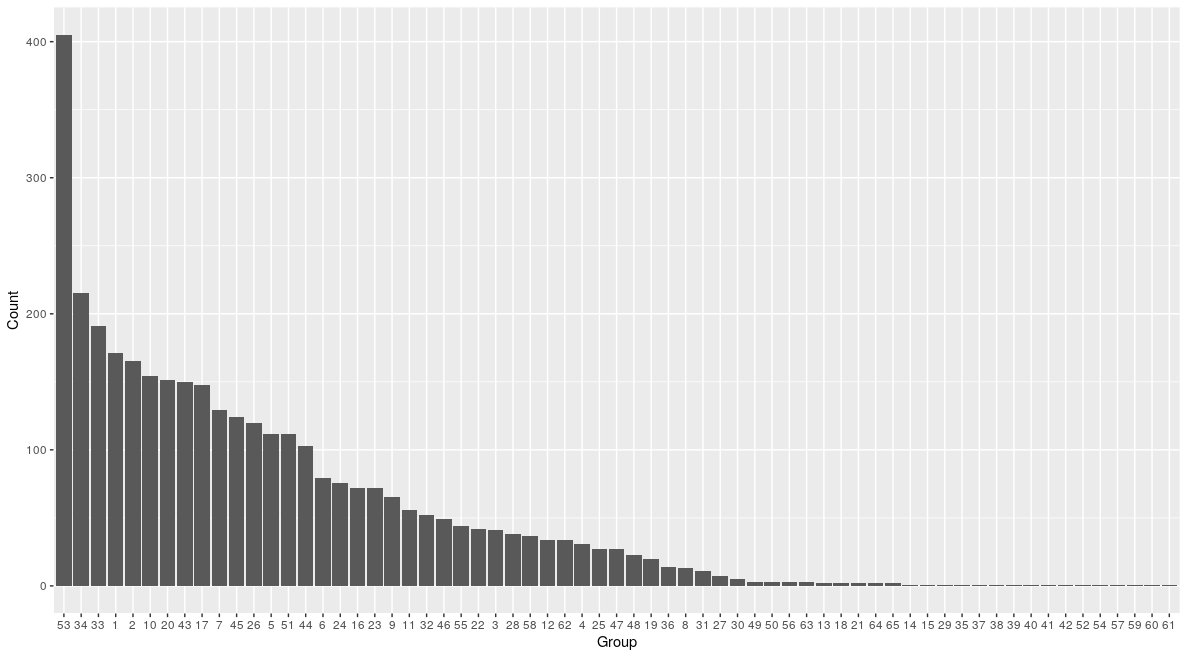
\includegraphics[width=\textwidth]{images/Rplot_group_size_spectral.png}
    \caption{Distribution of group sizes spectral clustering}
    \label{fig:group sizes spectral clustering shows power law distribution}
\end{figure}

\begin{figure}
    \centering
    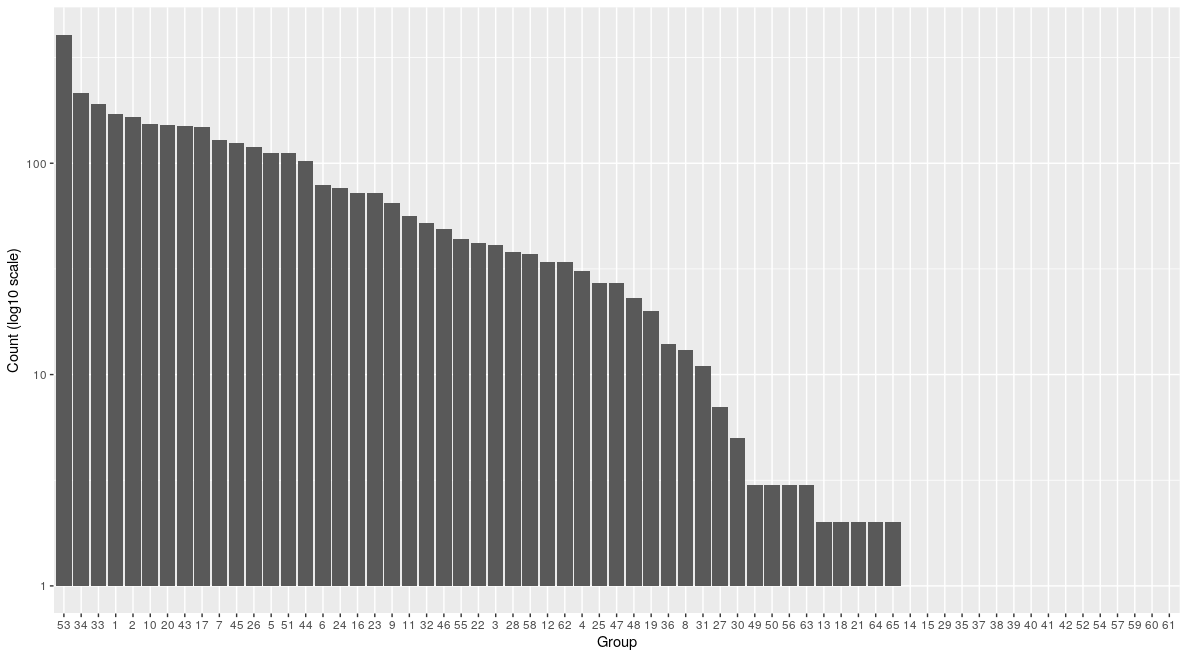
\includegraphics[width=\textwidth]{images/Rplot_spectral_groups_size_log10.png}
    \caption{Distribution of group sizes spectral clustering. Log 10 scaled y axis}
    \label{fig:group sizes spectral clustering log 10}
\end{figure}

% latex table generated in R 3.6.3 by xtable 1.8-4 package
% Wed Apr  8 11:31:09 2020

 
\subsection{pairwise comparison}

Table~\ref{tab:pairwise NMI on PSP} shows the Normalised Mutual Information between community allocation on the PSP for the graphs generated for the study (those carried out by Colin McLean). 

The NMI for lec (leading eigenvector method in igraph) and fast greedy are poor. 

% latex table generated in R 3.6.3 by xtable 1.8-4 package
% Mon Apr 12 13:30:15 2021
\begin{table}[ht]
\centering
\begin{adjustbox}{width=\textwidth}

\setlength{\extrarowheight}{2pt}
\begin{tabular}{lllllllllll}
  \toprule
& lec & wt & fc & sgG1 & sgG2 & sgG5 & Spectral & Geodesic & Louvain & infomap \\ 
  \midrule
lec & 1.000 & 0.172 & 0.185 & 0.160 & 0.132 & 0.128 & 0.191 & 0.235 & 0.165 & 0.145 \\ 
  wt & 0.172 & 1.000 & 0.291 & 0.366 & 0.467 & 0.520 & 0.456 & 0.661 & 0.399 & 0.631 \\ 
  fc & 0.185 & 0.291 & 1.000 & 0.327 & 0.268 & 0.256 & 0.280 & 0.341 & 0.243 & 0.324 \\ 
  sgG1 & 0.160 & 0.366 & 0.327 & 1.000 & 0.400 & 0.357 & 0.340 & 0.422 & 0.366 & 0.417 \\ 
  sgG2 & 0.132 & 0.467 & 0.268 & 0.400 & 1.000 & 0.595 & 0.443 & 0.578 & 0.423 & 0.537 \\ 
  sgG5 & 0.128 & 0.520 & 0.256 & 0.357 & 0.595 & 1.000 & 0.482 & 0.689 & 0.412 & 0.620 \\ 
  Spectral & 0.191 & 0.456 & 0.280 & 0.340 & 0.443 & 0.482 & 1.000 & 0.587 & 0.356 & 0.494 \\ 
  Geodesic & 0.235 & 0.661 & 0.341 & 0.422 & 0.578 & 0.689 & 0.587 & 1.000 & 0.462 & 0.663 \\ 
  Louvain & 0.165 & 0.399 & 0.243 & 0.366 & 0.423 & 0.412 & 0.356 & 0.462 & 1.000 & 0.445 \\ 
  infomap & 0.145 & 0.631 & 0.324 & 0.417 & 0.537 & 0.620 & 0.494 & 0.663 & 0.445 & 1.000 \\ 
   \bottomrule
\end{tabular}
\end{adjustbox}
\caption[Pairwise NMI for clustering algorithms on PSP]{Pairwise NMI on PSP. lec=Leading eigenvector method, wt = walktrap, fc = fast greedy CMN, sgG1-5 spingglass with Gamma 1,2 or 5, Geodesic - geodesic edge betweenness, louvain - louvain or multilevel} 
\label{tab:pairwise NMI on PSP}
\end{table}


\begin{table}[ht]
\centering
\begin{adjustbox}{width=\textwidth}

\setlength{\extrarowheight}{2pt}
\begin{tabular}{lrrrrrrrrrr}
\toprule
{} &  lec &   wt &   fc &  sgG1 &  sgG2 &  sgG5 &  Geodesic &  Spectral &  Louvain &  infomap \\
\midrule
lec      & 1.00 & 0.07 & 0.15 &  0.12 &  0.08 &  0.07 &      0.02 &      0.12 &      0.12 &     0.08 \\
wt       & 0.07 & 1.00 & 0.13 &  0.19 &  0.29 &  0.27 &      0.12 &      0.27 &      0.22 &     0.47 \\
fc       & 0.15 & 0.13 & 1.00 &  0.28 &  0.18 &  0.14 &      0.04 &      0.19 &      0.19 &     0.20 \\
sgG1     & 0.12 & 0.19 & 0.28 &  1.00 &  0.31 &  0.23 &      0.06 &      0.25 &      0.33 &     0.28 \\
sgG2     & 0.08 & 0.29 & 0.18 &  0.31 &  1.00 &  0.45 &      0.08 &      0.40 &      0.35 &     0.43 \\
sgG5     & 0.07 & 0.27 & 0.14 &  0.23 &  0.45 &  1.00 &      0.10 &      0.33 &      0.28 &     0.41 \\
Geodesic & 0.02 & 0.12 & 0.04 &  0.06 &  0.08 &  0.10 &      1.00 &      0.09 &      0.06 &     0.15 \\
Spectral & 0.12 & 0.27 & 0.19 &  0.25 &  0.40 &  0.33 &      0.09 &      1.00 &      0.28 &     0.37 \\
Louvain & 0.12 & 0.22 & 0.19 &  0.33 &  0.35 &  0.28 &      0.06 &      0.28 &      1.00 &     0.32 \\
infomap  & 0.08 & 0.47 & 0.20 &  0.28 &  0.43 &  0.41 &      0.15 &      0.37 &      0.32 &     1.00 \\
\bottomrule
\end{tabular}
\end{adjustbox}
\caption{Adjusted NMI for PSP. Including only those groupings done by CMcL}
\tiny\url{/home/grant/Projects_/Python/src/adjusted_nmi.ipynb}
\label{tab:adjusted NMI for PSP}
\end{table}


\subsection{Results Louvain group}
Louvain clustering discovers 14 communities in the PSP. The modularity of the resulting division is 0.339. 

The largest community is 539 genes in size (module 8). The minimum community size is 21 genes (module 12). The median module size is 190.5 and the mean is 246.9. The distribution of community sizes is shown in the boxplot in figure~\ref{fig:barplot_size_commmunities_using_louvain} code \url{source('~/RProjects/graph2community/R/plots/louvain_size.R')}
\subsection{results louvain fortunato}
Statistics for the communities following Fortunato \cite{fortunato2016community} are shown in table\ref{tab:Community statistics after fortunato louvain clustering}.

\begin{figure}
    \centering
    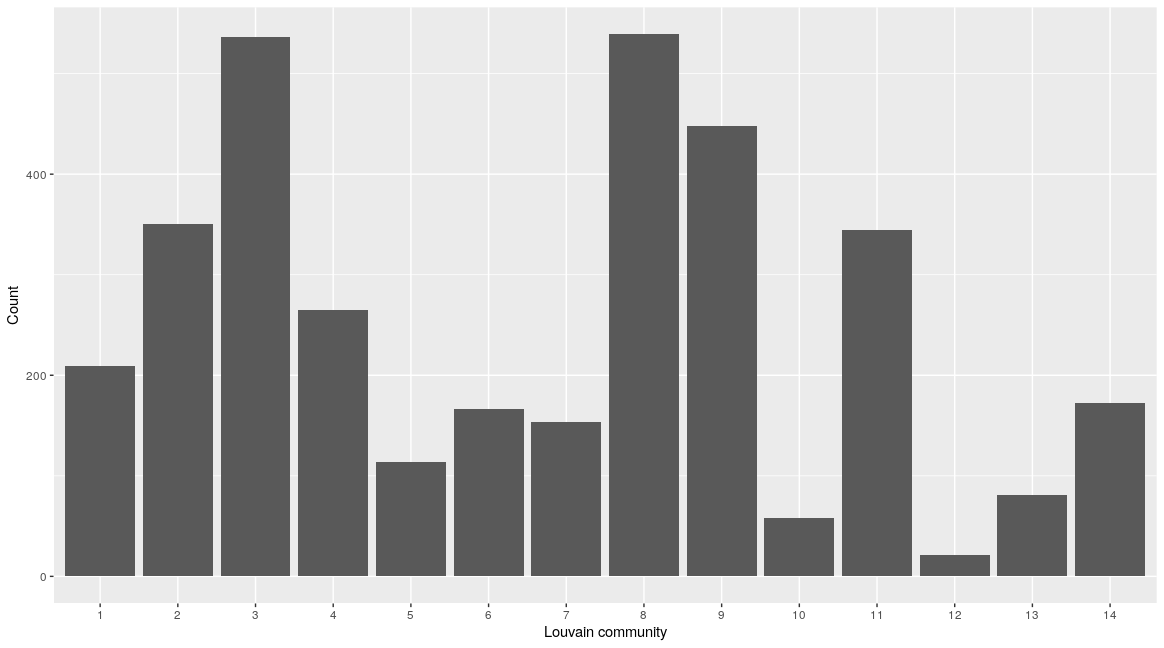
\includegraphics[width=\textwidth]{images/Rplot_Louvain_community_sizes.png}
    \caption{Barplot of the size of communities from the PSP discovered using the Louvain clustering method implemented in igraph}
    \label{fig:barplot_size_commmunities_using_louvain}
\end{figure}





\subsubsection{Spectral clustering community statistics for PSP}

The community statistics for the communities detected in the PSP using the spectral clustering method are shown in table~\ref{tab:Community statistics for Spectral following Fortunato.}.

Check that the volume is equal to 2 x the edge count  TRUE 
% latex table generated in R 3.6.3 by xtable 1.8-4 package
% Mon Jul 13 16:45:50 2020


\subsubsection{Results infomap group}
\label{sec:infomap_results}

Infomap discovers 171 communities. Group size  Min. 2.00, 1st  Qu.5.00,   Median 8.00,     Mean 20.2,2 3rd Qu. 13.00 ,  Max. 1228.00

The partition results in a large number of small communities. 

The modularity of the partition is 0.275.
 \todo{mean conductance of louvain,spectral and infomap}
\subsubsection{ InfoMap Result PSP}
On the PSP there are 171 groups the majority less than fifteen members in size, the median group size is 9 and mean 20.2. THe largest group is 1228 and the next largest 130. The conductance of the largest group is low compared to mean group conductance at 0.255 OTHER WAY ROUND  suggesting this large group is not very cohesive and the clustering may be suboptimal for our purposes. 

\subsubsection{results infomap fortunato}
For community statistics for modules with 15 or more members following Fortunato \cite{fortunato2016community} see table~\ref{tab:Community statistics after fortunato infomap clustering size > 15}



\section{Benchmarks}

\subsection{Community statistics}
\label{sec:Fortunato community statistics}

\cite{leskovec2010empirical}
In the same way that we were interested in importance measures for individual nodes in the previous chapters we are interested in measures of the properties of the discovered communities in addition to the global modularity property ($Q$)

A number of statistics can be calculated to characterise the properties of the communities detected such as how much they form a cohesive group isolated from the rest of the graph (conductance) and the number of edges outwith the group and within the group\cite{fortunato2016community}. Statistics can also be calculated for individual vertices showing their relation to the community (for example are they well embedded in the community or peripheral). The notation here follows Fortunato\cite{fortunato2016community} exactly and is for illustrative purposes \todo{ask JDA I mean this is pretty much verbatim the equations but these are the definitions}

The following are defined on communities

Internal connectedness
\begin{itemize}
    \item Internal degree $k_c^{int}$
    \begin{equation}
        k_c^{int}=\sum_{i,j\in C}A_{i,j}
    \end{equation}
    \item Average internal degree $k_c^{avg-int}$
    \begin{equation}
        k_c^{avg-int}=\frac{k_C^{int}}{n_c}
    \end{equation}
    \item Internal edge density $\delta_C^{int}$ The ratio of the number of internal edges to all possible internal edges $n_c(n_c-1)$
    \begin{equation}
        \delta_C^{int} = \frac{k_c^{int}}{n_C(n_C-1)}
    \end{equation}
    \end{itemize}
    External connectedness measures 
    \begin{itemize}
    \item External degree or \textit{cut} $k_c^{ext}$
    \begin{equation}
    k_c^{ext}=\sum_{i \in C, j \notin C}A_{i,j}
    \end{equation}
    \item Average external degree $k_c^{avg-ext}$ or \textit{expansion}
    \begin{equation}
        k_c^{avg-ext}=\frac{ k_c^{ext}}{n_C}
    \end{equation}
    \item External degree density or \textit{cut ratio} $\delta_C^{ext}$. The ratio of external degree to all possible external edges $n_c(n-n_c)$
    \begin{equation}
        \delta_C^{ext}=\frac{ k_c^{ext}}{n_C(n_C-1)}
    \end{equation}
    \end{itemize}
 Other 
    \begin{itemize}

    \item Total degree or \textit{volume} $k_c= k_c^{int}+k_c^{ext}$
    \item Average degree $k_c^{avg}$
    \begin{equation}
        k_c^{avg}=\frac{k_C}{n_C}
    \end{equation}
    \item Conductance
    
    \begin{equation}
    C_c = \frac{k_c^{ext}}{k_c}
    \label{eq:conductance}
    \end{equation}
    where $c$ represents community and $k$ degree, $n$ is the number of nodes in the graph and $n_c$ in community $c$
\end{itemize}




Vertex measures can also be calculated for individual vertices. Vertex internal and external degree are number of edges of a vertex linked to a member of the community or outwith the community respectively. Embeddedness $\zeta$ is the ratio of the internal degree to degree for a vertex and the mixing parameter $\mu$ is the ratio of external degree to the degree of a vertex\cite{fortunato2016community}.

What these measures provide are measures to assess the nature and quality of communities across a partition rather to augment the modularity which allows us to look at the global quality of the partition. This will help select an algorithm or algorithms for use in community based GSA by choosing algorithms that have desirable properties distributed throughout groups rather than concentrated in a single group (for example a low conductance - equation~\ref{eq:conductance})
\subsection{Observations from Fortunato}

\subsection{Performance on PSP network}
\label{sec:Performance on PSP network}
See table~\ref{tab:modularity and group sizes xtable} 

code \url{source('~/RProjects/group_sizes/R/make_clusterings/make_clusterings.R')}



\subsection{Benchmark: Stochastic block model Modularity and Group size}
\label{sec:benchmark sbm}

To investigate the difference in the performance of algorithms such as infomap on the LFR benchmark and on the PSP I analysed their performance on a block stochastic network model with increasing levels of background noise. Here I present the results of the infomap and Louvain method (infomap as it performed well in the benchmark and Louvain as it had relatively good performance on the PSP and has a short running time). I have calculated the normalised mutual information (NMI - not adjusted for chance) for the communities detected compared to ground truth. The test graph has 1000 vertices and a preference matrix where the probability of an edge is 0.1 if the nodes are in the same group and the chance of an edge if the nodes are not in the same group (background rate) varies between 0.001 and 0.1 in 0.001 steps.

Similar results were presented by \cite{yang2016comparative} using the LFR and changing the mixing parameter but the SBM allows demonstration of the exact probability rather than the mixing parameter which I find more intuitive\footnote{it can also be implemented along with the clustering algorithms in igraph}. 



Figure~\ref{fig:my_nice_infomap} shows perfect performance for the infomap algorithm as measured by NMI until the background probability reaches $p$=0.017. The NMI then falls to zero as infomap assigns all of the nodes to a single community. By contrast with the Louvain algorithm (figure~\ref{fig:my_sbmlouvain_nmi} the performance is not as good as infomap in the region where the background $p$ is less than 0.017 but above 0.017 the Louvain algorithm continues to perform tolerably well until over 0.05. Infomap performs very well (perfectly) when there is no `noise' but fails completely as background noise increases. We see a very similar picture in the PSP. 



\begin{figure}
    \centering
    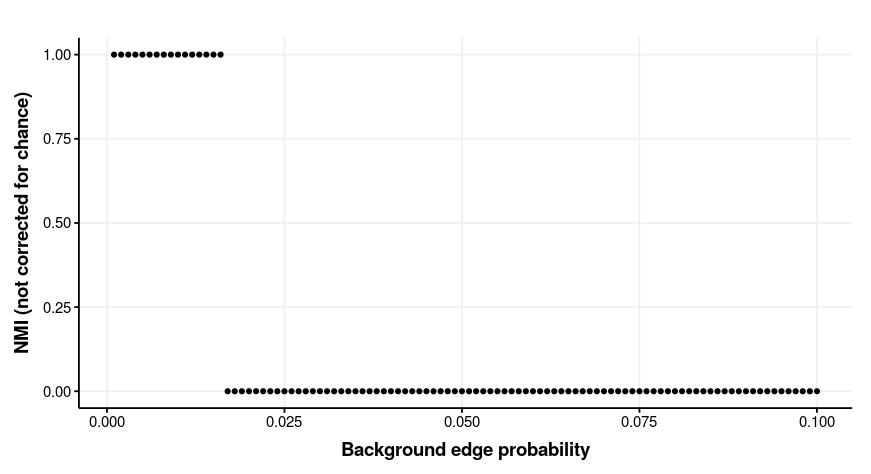
\includegraphics[width=\textwidth]{images/chaptercommunity/ggplot2/sbm_benchmark/Rplot_infomap_sbmtwogroups_theme.png}
    \caption{Diagnostics for infomap. Block stochastic model of two groups one 30\% of nodes other 70\% of nodes. Probability of edge between nodes in group $p$=0.1. x axis shows the probability of edge between nodes when they are in different groups (background probability). At 0.1 on x axis would be identical with probability in group. Graph shows dramatic decline in performance when background probability reaches $p$=0.017.}
    \tiny\url{source('~/RProjects/group_sizes/R/sbm_benchmark/two_groups_infomaprds.R')}
    \label{fig:my_nice_infomap}
\end{figure}


% \begin{figure}
%     \centering
%     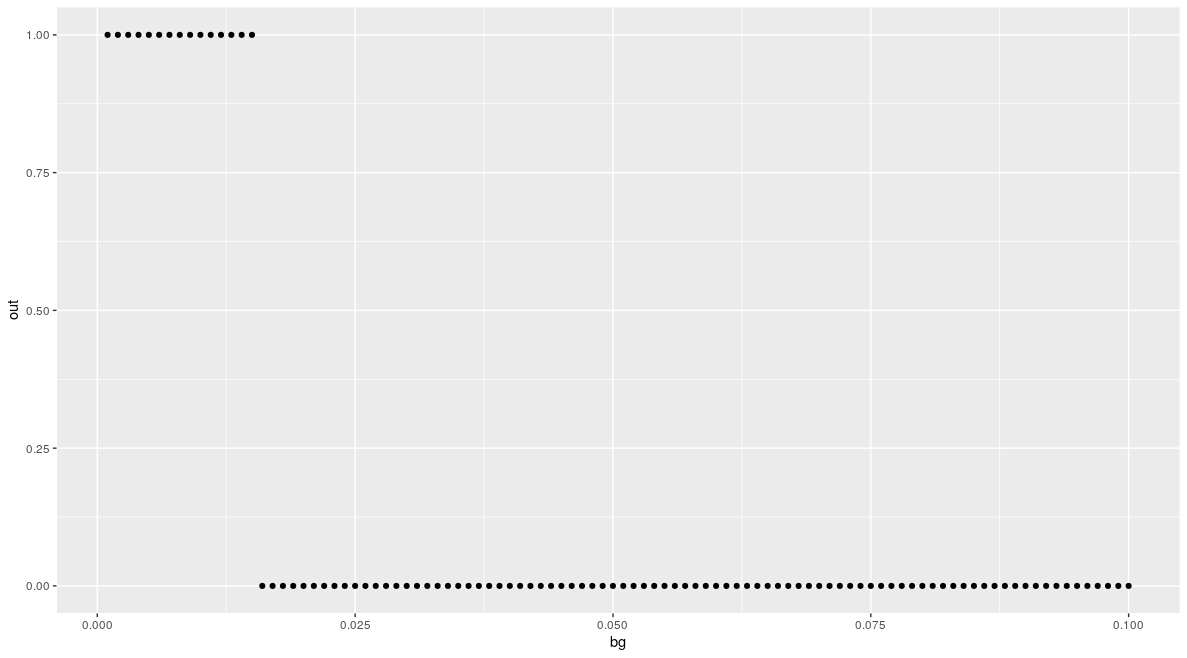
\includegraphics[width=\textwidth]{images/Rplot_rough_infomap_nmi_sbm.png}
%     \caption{NMI detected 2 (as out) group SBM infomap as approaches resolution limit. plot is p}
%     \tiny\url{source('~/RProjects/group_sizes/R/sbm_benchmark/two_groups_infomaprds.R')}
%     \label{fig:my_rough_infomap}
% \end{figure}


\begin{figure}
    \centering
    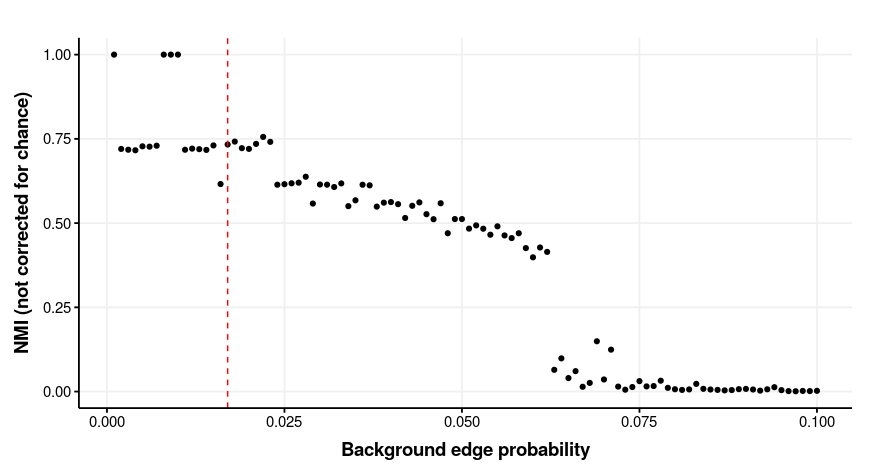
\includegraphics[width=\textwidth]{images/chaptercommunity/ggplot2/sbm_benchmark/Rplot_NMI_louvain.png}
    \caption{Diagnostics for Louvain clustering. Block stochastic model of two groups one 30\% of nodes other 70\% of nodes. Probability of edge between nodes in group $p$=0.1. x axis shows the probability of edge between nodes when they are in different groups (background probability). There is a gradual decline in the value of NMI ion contrast to the infomap figure~\ref{fig:my_nice_infomap}. Red dashed line represents background probability $p$=0.017 at which infomap performance dramatically decreases. In \cite{yang2016comparative} for LFR}
    \tiny\url{source('~/RProjects/group_sizes/R/sbm_benchmark/two_groups_louvainrds.R')}
    \label{fig:my_sbmlouvain_nmi}
\end{figure}



\begin{figure}
    \centering
    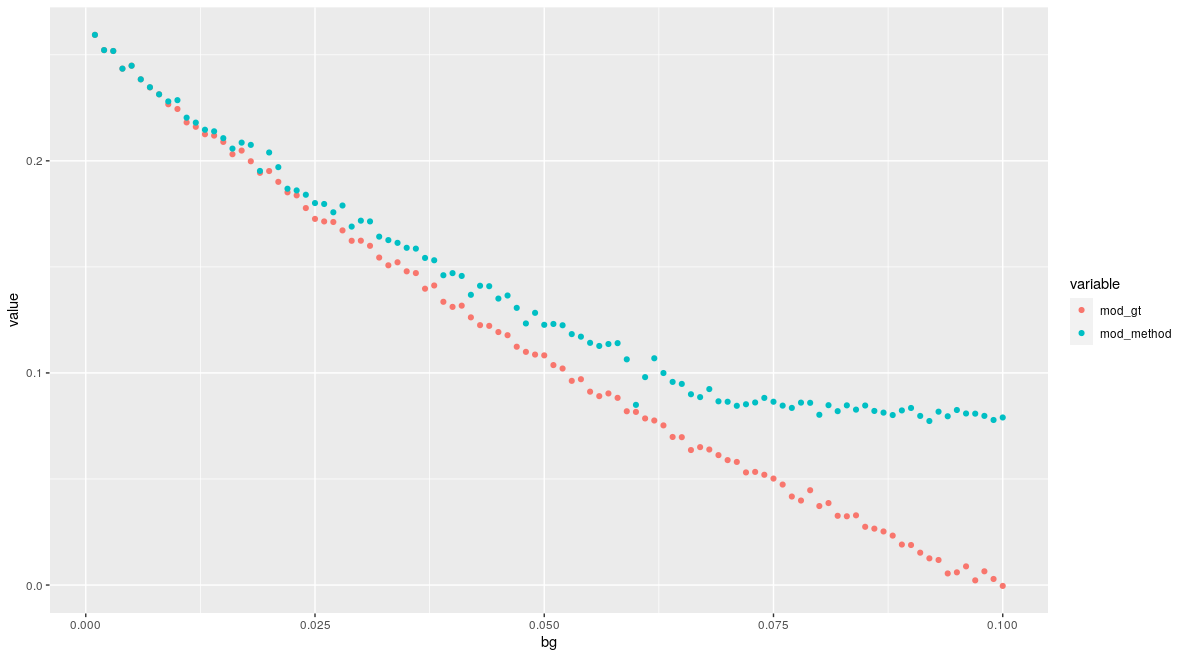
\includegraphics[width=\textwidth]{images/Rplot_rough_modularity_lou_ground_truth.png}
    \caption{Modularity group SBM louvain as approaches resolution limit. plot is p on x axis}
    \label{fig:my_rough_louvain modularity}
\end{figure}

\begin{figure}
    \centering
    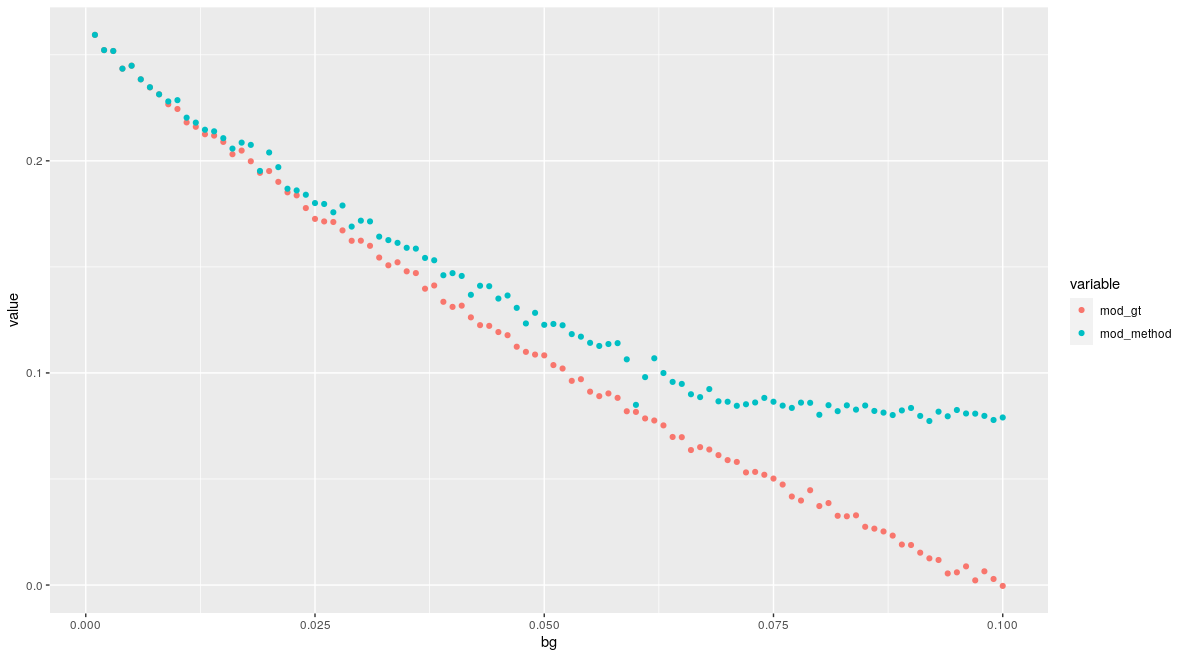
\includegraphics[width=\textwidth]{images/Rplot_rough_modularity_lou_ground_truth.png}
    \caption{Modularity group SBM louvain as approaches resolution limit. plot is p on x axis}
    \label{fig:my_rough_louvain modularity}
\end{figure}


\begin{figure}
    \centering
    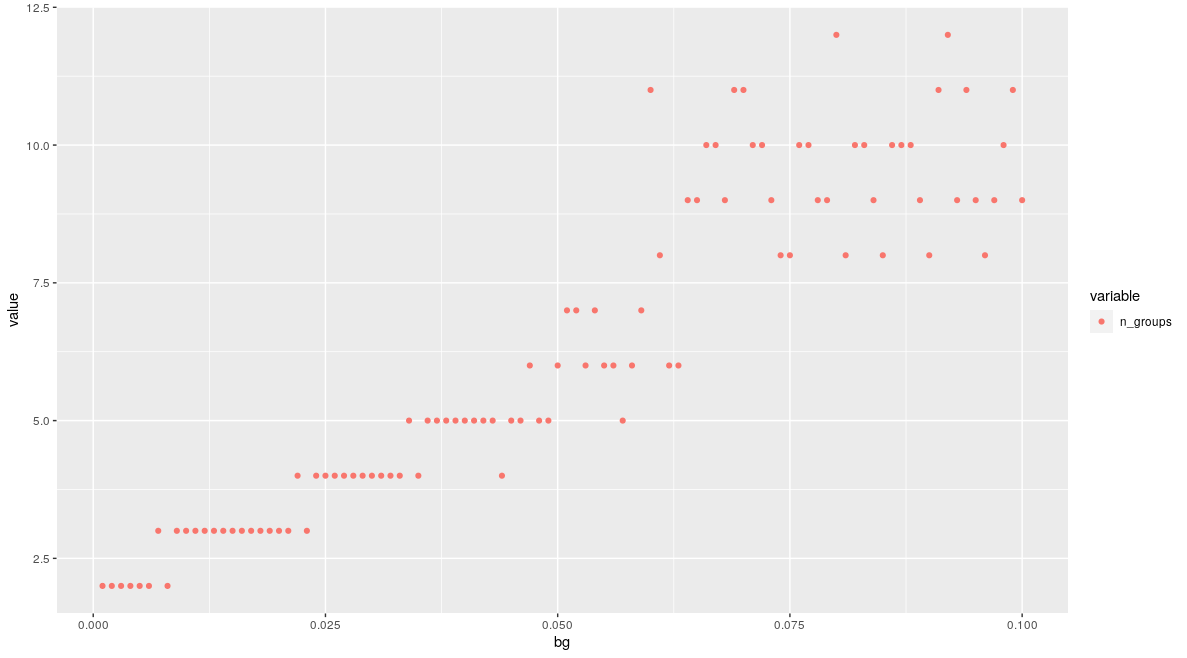
\includegraphics[width=\textwidth]{images/Rplot_group_size_rough_louvain_sbm.png}
    \caption{2 group SBM group size louvain as approaches resolution limit. plot is p on x axis see \url{source('~/RProjects/group_sizes/R/sbm_benchmark/graph/graph_performance_multi.R')}}
    \label{fig:my_rough_louvain group size}
\end{figure}

\subsubsection{Community detection thresholds}
\label{sec:community detection thresholds}
There are limits to the detection of communities specifically in the difference between the probability of edges and the probability of in group edges.

Newman p 512

\begin{equation}
    K1K2 < 2m
\end{equation}

Ie fails to detect separate communities if the product of the sum their degrees is less than 2m

So when increasing the background amount we are increasing m

\section{Methods for paper}
\label{sec: community detection methods from paper}
To study the effect of synaptic network structure on the genetics of cognitive ability and educational attainment we have used a discovery and replication cohort design. To understand how the structure of the PSP might affect the genetic architecture of these complex phenotypes, we first tested if there was an association between measures of the influence of individual vertices (gene) in the graph (degree), and their significance in GWA studies. 
Next, we used GSA to test whether the genes encoding proteins forming community structures in the network were significantly associated with differences in intelligence or educational attainment. 


\section{Cohorts and samples}

The GWA study samples used to test the association of centrality measures with population studies of educational attainment and intelligence were those described in sections~\ref{sec:cohorts from paper section} and \ref{sec:samples from paper section}


\section{Community detection method}
\label{sec:community detection method paper section}

I used the C++ implementation of spectral clustering with a fine tuning step () as it previously provided the best balance of performance and informative functional enrichment on synaptic proteome networks\cite{mclean2016improved}, community size on the PSP and performance on benchmark. 

Community detection was carried out using the CDS package as described in \cite{mclean2016improved} using ECDF, the distributed computing facility provided by the University of Edinburgh. All other analysis was performed on an Intel® Core™ i7-7700K CPU @ 4.20GHz 8 core workstation running Ubuntu 16.04 LTS 64 bit.  
The modularity was calculated in igraph library for R\cite{csardi2006igraph}. 

\subsection{Study design Topology based GSA}
\label{sec:Study design topology based GSA}
To test the hypothesis that there are network communities enriched for genes with genetic variants associated with intelligence or educational attainment we carried out the following procedures.

Communities of genes within the PSP are identified using spectral clustering. Gene based statistics were calculated (section~\ref{sec:MAGMA gene level methods} for discovery and replication samples and GSA performed (see \ref{sec:Gene set enrichment analysis} ) using the spectral communities as gene sets to identify potential communities of interest. PSP communities of interest are then tested in independent replication cohorts with correction for multiple hypothesis testing. The study design is shown in figure ~\ref{fig:study design community detection}.

\begin{figure}
    \centering
    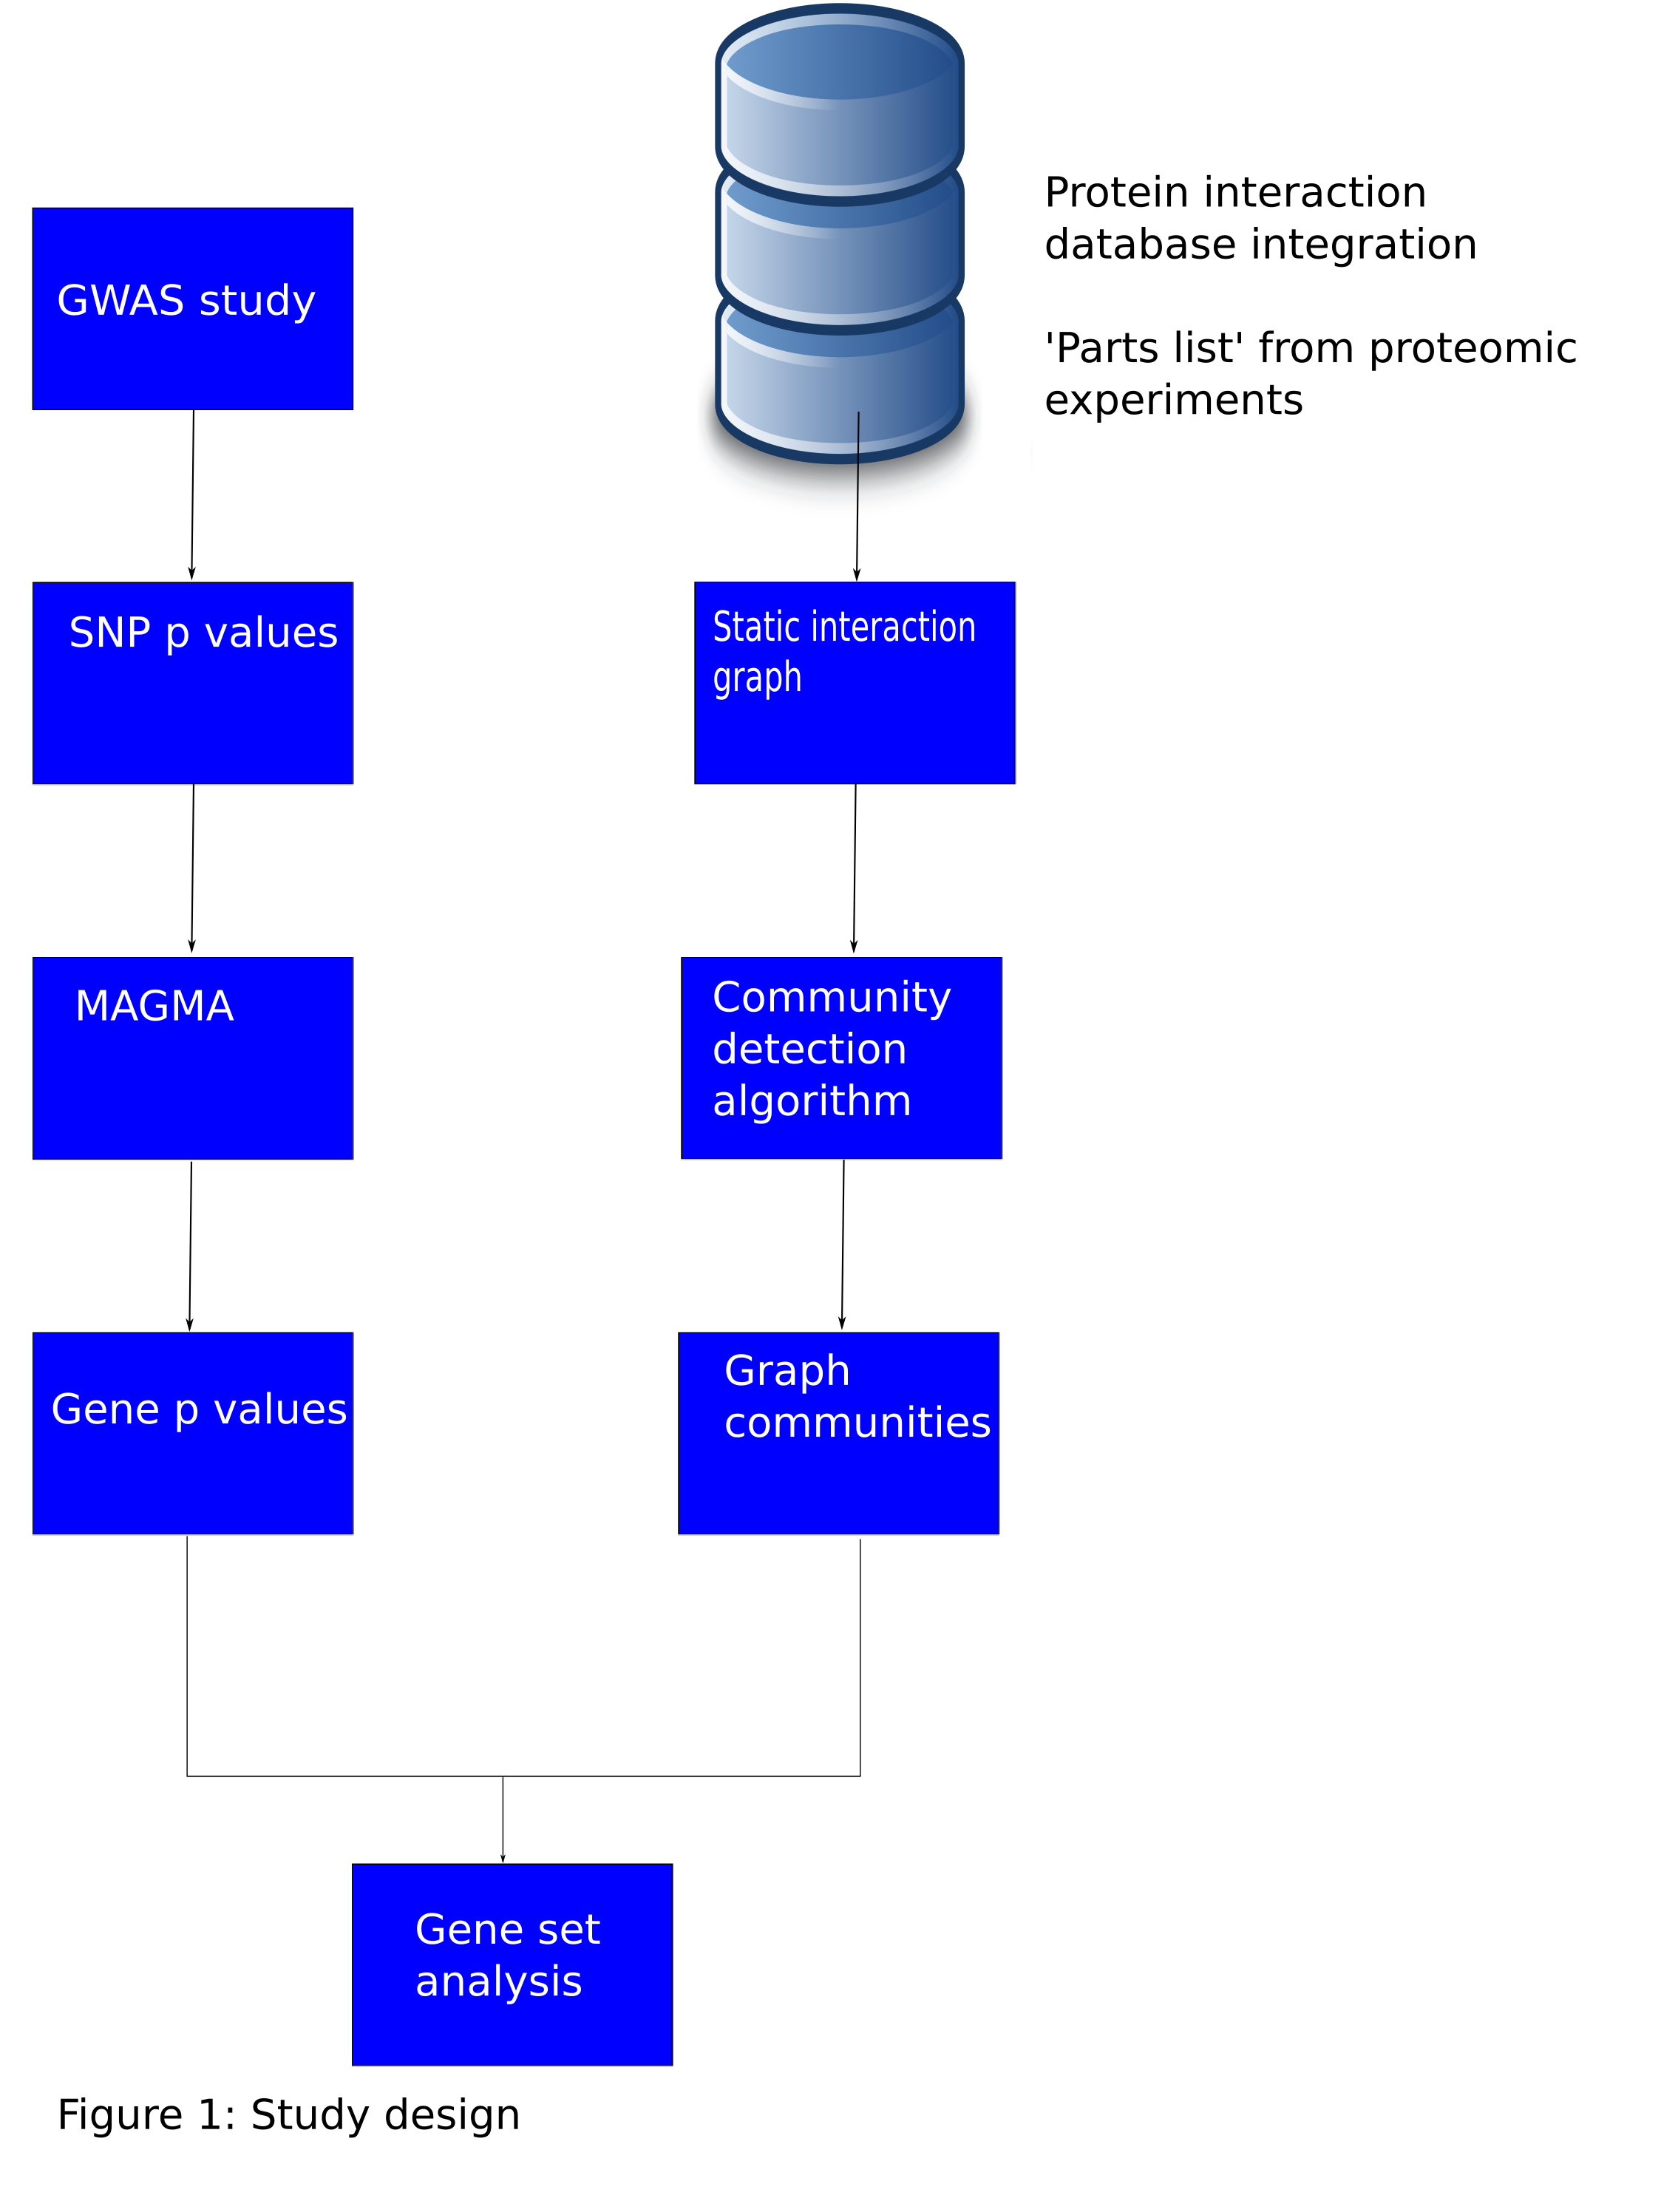
\includegraphics[width=\textwidth]{images/study_design.png}
    \caption{Study design}
    \label{fig:study design community detection}
\end{figure}

Community detection was carried out by Dr Colin McLean and recorded as vertex properties in a gml file. Dr McLean was blind to the results of the gene based analysis which I carried out based on the summary GWAS data. The communities in the gml file were converted to a gmt file using a custom R script. 



\subsubsection{PASCAL}
\label{sec:PASCAL community detection}
In order to determine if the choice of software for deriving a gene-based statistic influenced our results, we repeated our analyses using PASCAL instead of MAGMA, to provide both a gene level statistic and a competitive test of gene set enrichment\cite{lamparter2016fast}. The methods can be found in section~\ref{sec:PASCAL methods}.

 The instructions supplied to the program are available in the supplementary material as a shell script. 

\subsection{Gene set selection}
We used the non-overlapping communities generated by the spectral community detection algorithm as gene sets stored in .gmt file format (each row a gene set). We represented each protein in the community by the Entrez ID representing the gene encoding that protein. 

We selected gene sets with more than fifteen members. Divisive algorithms are known to often produce numerous small communities and small gene sets can result in the signal being dominated by a single gene. We used the default lower limit gene size for the Gene Set Enrichment Analysis software, GSEA, as the lower limit ($n$=15). 

\subsection{Gene-set analysis}
\label{sec:Gene set analysis community detection}
We carried out gene set analysis using the inbuilt GSA function implemented in MAGMA (section~\ref{sec:GSA MAGMA} and using the non -parametric competitive method implemented in GSEA which has been described in section~\ref{sec:Gene set enrichment analysis}\cite{de2015magma},\cite{subramanian2005gene}.  GSA in MAGMA implementation was as described in section~\ref{sec:Synaptic component enrichment MAGMA} except using spectral communities as gene sets\footnote{script is \url{run_gsa_mod.sh}}.   We followed the advice of Wilmot and Mooney and used more than one enrichment method utilising GSEA to provide a non- parametric enrichment analysis \cite{subramanian2005gene},\cite{mooney2015gene} (section~\ref{sec:Gene set enrichment analysis}).  Gene set enrichment analysis was carried out using the command line interface for the Java implementation of GSEA (GSEA - 3.0). To benchmark the performance of GSEA we ensured we could replicated the findings of Hill et al\cite{hill2014functional}.  The script to carry out the gene set analysis is included in the supplemental materials. 

We had no prior belief which, if any, communities would be associated with either phenotype. We therefore identified a set of genes (community) to be of interest if it attained nominally significant enrichment when tested using both MAGMA GSA and GSEA (see discussion section~\ref{sec:study design discussion}). These gene sets were then used in the Intelligence\textsubscript{Replication and }Education\textsubscript{Replication} samples with correction  for multiple testing using the Bonferroni method. Finally, the analysis pipeline was re-run using a different method of gene and pathway scoring (PASCAL) to test whether the findings were specific to a particular analysis platform\cite{lamparter2016fast}.  







\subsection{Gene ontology enrichment}
\label{sec:gene ontology methods from chapter community detection}
To investigate the nature and function of significant community modules we used gene ontology enrichment analysis (see section~\ref{sec: gene ontology analysis})\cite{mi2013large}.  

 We tested for over representation of Gene Ontology terms in significant communities (sets) for each of the major Gene Ontology clades using Fishers exact test with corrections for multiple comparisons using the FDR method calculated using ToppGene\cite{chen2009toppgene} using the other 3457 genes in the PSP as the background set (section~\ref{sec:ToppGene GO enrichment}). The ToppGene enrichment package was also used to perform enrichment analysis of significant communities for murine and human phenotypes with the PSP as the background set\cite{chen2009toppgene}.  

Evolutionary constraint in significant communities was assessed using the probability of loss of function intolerance for PSP genes using Gnomad v2.1.1 described in section\ref{sec:methods exac and gnomad}.


\section{Results}

The properties of the PSP network have been described in detail in chapter 3. It consists of 3457 nodes and 30498 edges. 

\subsubsection{Spectral community detection}
65 post synaptic graph communities (clusters) were detected using the spectral clustering algorithm with fine-tuning step; the modularity (Q) of the partition was 0.30 indicating a robust community architecture.  The communities ranged in size from 1 to 405 genes (mean 53.2, median 27, standard deviation 73). We excluded those communities with less than 15 members, removing 35 communities and 88 genes (2.5\% of the PSP). 35 communities with a total of 3369 genes remained with mean community size 96.1, median 72 and standard deviation 76.8 (see section~\ref{sec:Performance on PSP graph} and table~\ref{tab:modularity and group sizes PSP xtable}). For community statistics following Fortunato \cite{fortunato2016community} see table~\ref{tab:Community statistics for Spectral following Fortunato.} 


\begin{figure}
    \centering
    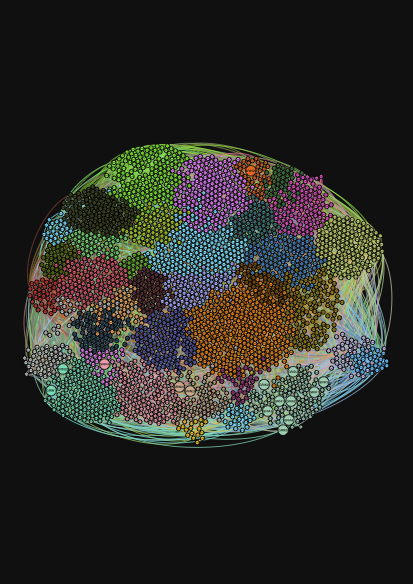
\includegraphics[width=0.9\textwidth]{images/chapter_community_detection/from_slides/network_png_50.png}
    \caption{Placeholder picture of communities low pixel per inch (50)}
    \label{fig:communities_spectral}
\end{figure}


% latex table generated in R 3.6.3 by xtable 1.8-4 package
% Tue Apr  7 17:38:02 2020


\subsection{Gene set enrichment results}
In order to test the hypothesis that particular topological groups within the graph (communities) are enriched for genetic variants associated with differences in educational attainment or intelligence we carried out competitive Gene Set Analysis using the topological communities as gene sets. 


Four of 35 communities showed greater than nominally ($p$<0.05) significant enrichment using MAGMA GSA in the Education Discovery cohort (community: 5, $p$\textsubscript{MAGMA}=0.002, number of genes=106; community 53 $n$=405, community 22 $n$=42, P\textsubscript{MAGMA}=0.034; cluster 47 P\textsubscript{MAGMA}= 0.035 n=47). These communities other than 53 were among the 8 showing nominally significant enrichment using GSEA (2,5,11,20,22,24,33,47) and so communities 5, 22 and 47 (PGSEA= 0.004 ,0.014, 0.017) were taken forward to the replication cohorts. PGSEA for community 53 was 0.29. 

% latex table generated in R 3.6.3 by xtable 1.8-4 package
% Sun Apr  4 13:58:07 2021

\begin{table}[ht]
\centering
\setlength{\extrarowheight}{2pt}
\begin{tabular}{cllllllllll}
  \toprule
   &  \multicolumn{5}{c}{\textit{Discovery}} & \multicolumn{5}{c}{\textit{Replication}} \\
    \cmidrule{2-11}
Community & $n$ & $\beta$ & $\beta$ STD & SE & $p$ & $n$ & $\beta$ & $\beta$ STD & SE & $p$\\ 
  \midrule
1 & 161 & -0.03 & -0.00 & 0.07 & 0.639 & 162 & 0.05 & 0.01 & 0.07 & 0.207 \\ 
  2 & 153 & 0.10 & 0.01 & 0.08 & 0.093 & 153 & -0.07 & -0.01 & 0.07 & 0.867 \\ 
  3 & 39 & 0.22 & 0.01 & 0.16 & 0.082 & 39 & 0.09 & 0.00 & 0.14 & 0.260 \\ 
  4 & 29 & -0.17 & -0.01 & 0.18 & 0.821 & 30 & -0.36 & -0.01 & 0.15 & 0.991 \\ 
  \textbf{5} & 106 & 0.22 & 0.02 & 0.10 & \textbf{0.014} & 106 & 0.21 & 0.02 & 0.09 & \textbf{0.009} \\ 
  6 & 76 & -0.07 & -0.00 & 0.12 & 0.715 & 77 & 0.09 & 0.01 & 0.10 & 0.170 \\ 
  7 & 125 & 0.14 & 0.01 & 0.09 & 0.052 & 125 & -0.08 & -0.01 & 0.08 & 0.840 \\ 
  9 & 61 & -0.01 & -0.00 & 0.12 & 0.545 & 61 & 0.23 & 0.01 & 0.11 & 0.016 \\ 
  \textbf{10} & 146 & 0.19 & 0.02 & 0.08 & \textbf{0.008} & 146 & 0.02 & 0.00 & 0.07 & 0.375 \\ 
  11 & 55 & 0.14 & 0.01 & 0.13 & 0.145 & 55 & -0.11 & -0.01 & 0.11 & 0.848 \\ 
  12 & 32 & -0.01 & -0.00 & 0.16 & 0.522 & 32 & 0.18 & 0.01 & 0.15 & 0.113 \\ 
  16 & 68 & 0.00 & 0.00 & 0.12 & 0.494 & 68 & 0.21 & 0.01 & 0.10 & 0.022 \\ 
  17 & 144 & 0.02 & 0.00 & 0.08 & 0.417 & 144 & -0.00 & -0.00 & 0.07 & 0.506 \\ 
  19 & 20 & 0.21 & 0.01 & 0.18 & 0.124 & 20 & 0.10 & 0.00 & 0.15 & 0.262 \\ 
  20 & 144 & 0.13 & 0.01 & 0.09 & 0.070 & 144 & 0.13 & 0.01 & 0.07 & 0.039 \\ 
  \textbf{22} & 42 & 0.24 & 0.01 & 0.14 & \textbf{0.047} & 42 & -0.06 & -0.00 & 0.13 & 0.669 \\ 
  23 & 67 & -0.08 & -0.00 & 0.12 & 0.741 & 67 & -0.17 & -0.01 & 0.10 & 0.954 \\ 
  24 & 74 & 0.10 & 0.01 & 0.12 & 0.191 & 74 & 0.18 & 0.01 & 0.10 & 0.032 \\ 
  25 & 26 & 0.01 & 0.00 & 0.19 & 0.487 & 26 & -0.03 & -0.00 & 0.16 & 0.582 \\ 
  26 & 117 & 0.10 & 0.01 & 0.09 & 0.130 & 116 & 0.06 & 0.00 & 0.08 & 0.245 \\ 
  28 & 35 & -0.04 & -0.00 & 0.17 & 0.603 & 35 & 0.34 & 0.01 & 0.15 & 0.011 \\ 
  32 & 50 & -0.05 & -0.00 & 0.15 & 0.635 & 50 & 0.10 & 0.01 & 0.12 & 0.200 \\ 
  33 & 180 & 0.05 & 0.00 & 0.07 & 0.270 & 180 & 0.10 & 0.01 & 0.06 & 0.062 \\ 
  34 & 210 & 0.06 & 0.01 & 0.07 & 0.216 & 211 & -0.09 & -0.01 & 0.06 & 0.937 \\ 
  43 & 137 & 0.02 & 0.00 & 0.08 & 0.389 & 139 & -0.03 & -0.00 & 0.07 & 0.656 \\ 
  44 & 101 & 0.02 & 0.00 & 0.09 & 0.434 & 101 & -0.00 & -0.00 & 0.08 & 0.505 \\ 
  45 & 118 & 0.09 & 0.01 & 0.09 & 0.139 & 119 & 0.03 & 0.00 & 0.07 & 0.335 \\ 
  46 & 47 & 0.07 & 0.00 & 0.12 & 0.283 & 47 & 0.06 & 0.00 & 0.10 & 0.264 \\ 
  47 & 23 & 0.22 & 0.01 & 0.20 & 0.132 & 24 & -0.05 & -0.00 & 0.18 & 0.619 \\ 
  48 & 22 & 0.03 & 0.00 & 0.20 & 0.445 & 22 & -0.05 & -0.00 & 0.21 & 0.592 \\ 
  51 & 110 & -0.06 & -0.00 & 0.09 & 0.750 & 110 & 0.13 & 0.01 & 0.08 & 0.038 \\ 
  53 & 386 & 0.08 & 0.01 & 0.05 & 0.050 & 387 & 0.08 & 0.01 & 0.04 & 0.024 \\ 
  55 & 42 & 0.22 & 0.01 & 0.15 & 0.069 & 42 & 0.04 & 0.00 & 0.12 & 0.371 \\ 
  58 & 36 & -0.10 & -0.00 & 0.16 & 0.738 & 36 & -0.01 & -0.00 & 0.14 & 0.543 \\ 
  62 & 34 & -0.06 & -0.00 & 0.15 & 0.656 & 34 & -0.18 & -0.01 & 0.14 & 0.905 \\ 
   \bottomrule
\end{tabular}
\caption{MAGMA GSA Intelligence  BETA is the regression coefficient of the gene set. SE is the standard error of the regression coefficient. BETA SD the the semi-standardized regression coefficient, corresponding to the predicted
change in Z-value given a change of one standard deviation in the predictor gene set  gene covariate } 
\tiny\url{source('~/RProjects/chapter_community_detection/R/magma_gsa/intelligence_gsa_table.R')}\\
Redo 2021 \url{source('~/RProjects/chapter_community_detection/R/magma_gsa/rawread/intelligence_gsa_new_raw_table.R')}
\label{tab:MAGMA GSA Intelligence }
\end{table}

See table 2 and supplementary tables 2 and 3. GSEA Educational attainment table~\ref{tab:Significant gene sets Educational Attaintment} and GSEA Intelligence table~\ref{tab:Significant gene sets GSEA Intelligence}.


In the Intelligence Discovery cohort three four gene sets showed nominally significant enrichment using MAGMA GSA (cluster 10, p=0.008, n=146; cluster 5 p=0.014, n=106; cluster 22 p=0.046; cluster 53 p=0.049). However, only group community 5 showed at least nominally significant enrichment on GSEA and was analysed in the replication cohort. 
Group Community 5 was confirmed to have an enriched association with educational attainment in the replication cohort P\textsubscript{MAGMA}=0.01548, P\textsubscript{MAGMA} permutation= 0.043. Community Group 5 genes also were enriched in the Intelligence\textsubscript{Replication cohort} (p = 0.0084).




\begin{table}[ht!]
\centering
\setlength{\extrarowheight}{2pt}
\begin{tabular}{lllllll}
  \toprule
   &  \multicolumn{3}{c}{\textit{Discovery}} & \multicolumn{3}{c}{\textit{Replication}} \\
   \cmidrule{2-7}
Set & $n$ & ES & $p$ & $n$ & ES & $p$ \\ 
  \midrule
24 & 73 & 0.61 & 0.002 & 73 & 0.58 & 0.004 \\ 
  33 & 179 & 0.54 & 0.002 & 179 & 0.52 & 0.003 \\ 
  5 & 105 & 0.58 & 0.006 & 105 & 0.52 & 0.015 \\ 
  47 & 22 & 0.70 & 0.009 &  &  &  \\ 
  20 & 143 & 0.55 & 0.015 & 141 & 0.52 & 0.005 \\ 
  22 & 41 & 0.62 & 0.018 &  &  &  \\ 
  11 & 54 & 0.58 & 0.024 &  &  &  \\ 
  55 &  &  &  & 41 & 0.64 & 0.003 \\ 
  9 &  &  &  & 60 & 0.59 & 0.006 \\ 
  43 &  &  &  & 136 & 0.52 & 0.014 \\ 
   \bottomrule
\end{tabular}
\caption{Significant gene sets. GSEA Educational Attaintment. Discovery and replication cohorts.  ES = Enrichment score. n = number of genes in gene set, $p$= nominal p value} 
\tiny\url{source('~/RProjects/chapter_community_detection/R/gsea/format_sig_educational.R')}
\label{tab:Significant gene sets Educational Attaintment}
\end{table}

% latex table generated in R 3.6.3 by xtable 1.8-4 package
% Tue Mar 30 17:09:20 2021
\begin{table}[ht!]
\centering
\setlength{\extrarowheight}{2pt}
\begin{tabular}{lllllll}
  \toprule
   &  \multicolumn{3}{c}{\textit{Discovery}} & \multicolumn{3}{c}{\textit{Replication}} \\
   \cmidrule{2-7}
Set & $n$ & ES & $p$ & $n$ & ES & $p$ \\ 
  \midrule
5 & 105 & 0.60 & 0.001 & 105 & 0.54 & 0.003 \\ 
  53 & 385 & 0.51 & 0.004 &  &  &  \\ 
  43 & 136 & 0.54 & 0.013 &  &  &  \\ 
  34 & 209 & 0.51 & 0.023 &  &  &  \\ 
  3 & 38 & 0.60 & 0.038 &  &  &  \\ 
  20 &  &  &  & 143 & 0.51 & 0.009 \\ 
  33 &  &  &  & 179 & 0.48 & 0.021 \\ 
  26 &  &  &  & 115 & 0.50 & 0.033 \\ 
   \bottomrule
\end{tabular}
\caption{Significant gene sets GSEA IntelligenceDiscovery and replication cohorts.  ES = Enrichment score. n = number of genes in gene set, $p$= nominal p value}
\tiny\url{source('~/RProjects/chapter_community_detection/R/gsea/format_sig_intelligence.R')}
\label{tab:Significant gene sets GSEA Intelligence}
\end{table}

Gene set enrichment tests were also performed using the pathway function in PASCAL.\cite{lamparter2016fast} Community Group 5 showed significant enrichment in all four cohorts using PASCAL’s gene scoring and GSA analysis methods Education Discovery p=0.00007, Intelligence Discovery p=0.0001; Education Replication p=0.0003, Intelligence Replication p=0.0001; alpha Bonferroni 0.0015 (Supplemental table 8). 

PASCAL XX table~\ref{tab:Intelligence PASCAL} and table~\ref{tab:Pascal Education ordered by chi2P}

% latex table generated in R 3.6.3 by xtable 1.8-4 package
% Sun Apr  4 14:43:19 2021
\begin{table}[ht]
\centering
\setlength{\extrarowheight}{2pt}
\begin{tabular}{llllll}
  \toprule
   &  \multicolumn{2}{c}{\textit{Discovery}} & \multicolumn{2}{c}{\textit{Replication}} \\
   \cmidrule{2-5}
 Name & chi2Pvalue  & empPvalue  & chi2Pvalue   & empPvalue   \\ 
  \midrule
5 & 0.00005 & 0.00011 & 0.00005 & 0.00012 \\ 
  10 & 0.00118 & 0.00842 & 0.00215 & 0.00238 \\ 
  53 & 0.00551 & 0.00674 & 0.05289 & 0.04662 \\ 
  7 & 0.01457 & 0.03852 & 0.23362 & 0.17917 \\ 
  33 & 0.02126 & 0.06174 & 0.03314 & 0.03936 \\ 
  26 & 0.02152 & 0.03371 & 0.09655 & 0.12936 \\ 
  20 & 0.02629 & 0.05821 & 0.00142 & 0.00239 \\ 
  34 & 0.03021 & 0.07349 & 0.48926 & 0.45609 \\ 
  28 & 0.06082 & 0.06805 & 0.18416 & 0.23682 \\ 
  43 & 0.06633 & 0.03141 & 0.37601 & 0.41863 \\ 
  55 & 0.08403 & 0.13622 & 0.44314 & 0.47030 \\ 
  22 & 0.09465 & 0.07006 & 0.32361 & 0.26264 \\ 
  3 & 0.09514 & 0.07290 & 0.13478 & 0.11655 \\ 
  19 & 0.09847 & 0.05388 & 0.88967 & 0.86107 \\ 
  58 & 0.12710 & 0.10808 & 0.26938 & 0.19509 \\ 
  2 & 0.13497 & 0.16725 & 0.76900 & 0.73094 \\ 
  45 & 0.13872 & 0.15079 & 0.43880 & 0.38630 \\ 
  12 & 0.14885 & 0.21203 & 0.13265 & 0.17448 \\ 
  11 & 0.15258 & 0.13086 & 0.90882 & 0.89701 \\ 
  24 & 0.17389 & 0.16971 & 0.04770 & 0.06090 \\ 
  46 & 0.18991 & 0.18483 & 0.20068 & 0.22571 \\ 
  47 & 0.26565 & 0.24708 & 0.34319 & 0.29384 \\ 
  1 & 0.29315 & 0.32094 & 0.21352 & 0.24257 \\ 
  9 & 0.31205 & 0.38279 & 0.07316 & 0.09553 \\ 
  23 & 0.33463 & 0.39840 & 0.64103 & 0.66756 \\ 
  32 & 0.33661 & 0.41270 & 0.17894 & 0.21654 \\ 
  44 & 0.36507 & 0.39839 & 0.57021 & 0.53741 \\ 
  17 & 0.37087 & 0.31369 & 0.35273 & 0.31447 \\ 
  25 & 0.44107 & 0.44977 & 0.44278 & 0.45825 \\ 
  51 & 0.45466 & 0.56525 & 0.07424 & 0.08153 \\ 
  62 & 0.65120 & 0.63921 & 0.47485 & 0.49011 \\ 
  48 & 0.65913 & 0.65999 & 0.82988 & 0.82570 \\ 
  16 & 0.73722 & 0.70116 & 0.08981 & 0.11902 \\ 
  6 & 0.76799 & 0.74957 & 0.39325 & 0.31039 \\ 
  4 & 0.80237 & 0.78159 & 0.96353 & 0.96408 \\ 
   \bottomrule
\end{tabular}
\caption{Intelligence PASCAL ordered by chi2Pvalue}
\label{tab:Intelligence PASCAL}
\end{table}


% latex table generated in R 3.6.3 by xtable 1.8-4 package
% Sun Apr  4 14:55:16 2021
\begin{table}[ht]
\centering
\setlength{\extrarowheight}{2pt}
\begin{tabular}{llllll}
  \toprule
   &  \multicolumn{2}{c}{\textit{Discovery}} & \multicolumn{2}{c}{\textit{Replication}} \\
   \cmidrule{2-5}
 Name & chi2Pvalue  & empPvalue  & chi2Pvalue   & empPvalue   \\ 
  \midrule
5 & 0.00006 & 0.00007 & 0.00101 & 0.00026 \\ 
  20 & 0.00009 & 0.00064 & 0.00019 & 0.00214 \\ 
  2 & 0.00010 & 0.00197 & 0.02859 & 0.05484 \\ 
  33 & 0.00033 & 0.00351 & 0.00774 & 0.03373 \\ 
  47 & 0.01040 & 0.03107 & 0.29248 & 0.30947 \\ 
  24 & 0.01135 & 0.00904 & 0.00121 & 0.00124 \\ 
  53 & 0.01668 & 0.03576 & 0.44041 & 0.57615 \\ 
  22 & 0.01690 & 0.04507 & 0.17748 & 0.17328 \\ 
  1 & 0.04775 & 0.04565 & 0.19103 & 0.20056 \\ 
  11 & 0.04848 & 0.02619 & 0.24541 & 0.10527 \\ 
  10 & 0.04947 & 0.12340 & 0.14220 & 0.12294 \\ 
  34 & 0.06379 & 0.09816 & 0.02931 & 0.08681 \\ 
  32 & 0.07427 & 0.14669 & 0.88655 & 0.88639 \\ 
  26 & 0.12693 & 0.11476 & 0.29690 & 0.21301 \\ 
  51 & 0.12879 & 0.19808 & 0.06750 & 0.10246 \\ 
  44 & 0.13406 & 0.21763 & 0.12548 & 0.22032 \\ 
  46 & 0.16189 & 0.17636 & 0.37360 & 0.40041 \\ 
  7 & 0.20011 & 0.23541 & 0.44014 & 0.47564 \\ 
  4 & 0.21800 & 0.27362 & 0.94031 & 0.93664 \\ 
  12 & 0.22076 & 0.24324 & 0.12664 & 0.19635 \\ 
  45 & 0.22085 & 0.33226 & 0.34137 & 0.41257 \\ 
  55 & 0.23156 & 0.31491 & 0.04923 & 0.05854 \\ 
  9 & 0.23518 & 0.32986 & 0.03420 & 0.07557 \\ 
  19 & 0.29122 & 0.33875 & 0.37543 & 0.39652 \\ 
  3 & 0.31886 & 0.27426 & 0.34172 & 0.35703 \\ 
  28 & 0.33989 & 0.36836 & 0.19262 & 0.26534 \\ 
  23 & 0.39185 & 0.47784 & 0.58355 & 0.61850 \\ 
  6 & 0.42214 & 0.46701 & 0.70931 & 0.70462 \\ 
  17 & 0.42623 & 0.47928 & 0.60287 & 0.57664 \\ 
  16 & 0.43234 & 0.51029 & 0.31117 & 0.42090 \\ 
  43 & 0.47397 & 0.47877 & 0.00273 & 0.00416 \\ 
  48 & 0.49223 & 0.46679 & 0.55516 & 0.56118 \\ 
  58 & 0.71790 & 0.74793 & 0.62110 & 0.65671 \\ 
  62 & 0.96246 & 0.96134 & 0.19788 & 0.25513 \\ 
  25 & 0.96330 & 0.96085 & 0.64162 & 0.65989 \\ 
   \bottomrule
\end{tabular}
\caption{Pascal Education ordered by chi2P} 
\label{tab:Pascal Education ordered by chi2P}
\end{table}
\clearpage

\clearpage
\subsection{Gene set enrichment results}

The raw output files are in \url{/home/grant/Programs/gsea_script/gsea_output/} need to bundle
\subsection{Gene ontology analysis}
\label{sec: spectral group 5 analysis}
We performed gene ontology enrichment analysis on community  5. Community 5 is significantly enriched for terms related to glutamate receptor activity and the heterotrimeric g protein complex, including the G protein coupled serotonin receptor. Community 5 has a significant proportion of these terms whether one compares against the rest of the genome or relative to other synaptic groups. 21 of the 27 genes annotated by the Gene Ontology Consortium as
glutamate receptor activity (GO:0008066 MF) are found in the PSP. Of these, 12 are found in group 5 (57.1\%). 
23 of the 37 genes encoding proteins annotated heterotrimeric g protein (GO:0005834) are found in the PSP. Of these, 16 are found in group 5 (69.5\% of PSP GO:0005834). 

The PANTHER over-representation test was carried out for each of the GO clades, Biological Process, Molecular Function, Cellular Component with the gene set compared with the 3457 PSP genes. The results are ordered by FDR and are presented in tables 9-11 in the supplemental material 

The biological process (BP) with the lowest FDR p value was G protein coupled receptor signalling activity, GO:0007186: FDR 2.16 x 10-8, fold enrichment 4.23. The second lowest was glutamate receptor signalling pathway GO 0007215: FDR 7.23 x 10-07, fold change 12.62.

Glutamate receptor activity GO:0008066 was also the most over represented molecular function term: FDR 7.58 x 10-07, fold change 16. The most enriched cellular component was GTPase complex GO:1905360: FDR 8.75 x 10-8, fold change 18.23. This was followed by heterotrimeric G-protein complex: FDR 1.75 x 10-7, fold change 18.23.

Enrichment analysis for ontology terms for Group 5 was also carried out with the entire genome  used to calculate the background frequency of terms (Panther default). Similar results with enrichment for g-protein associated receptors and glutamate receptors were found and shown in tables 12-14 in the supplemental material.
% latex table generated in R 3.6.3 by xtable 1.8-4 package
% Sun Apr  4 15:28:14 2021
% latex table generated in R 3.6.3 by xtable 1.8-4 package
% Sun Apr  4 15:35:07 2021
\begin{table}[ht]
\centering
\setlength{\extrarowheight}{2pt}
\begin{adjustbox}{width=\textwidth}
\begin{tabular}{llllll}
  \toprule
ID & Name & $n$ & $n$ PSP & $p$ & $q$ FDR B.H \\ 
  \midrule
GO:0008066 & glutamate receptor activity & 12 & 21 & $1.86 \times 10^{-13}$ & $6.96 \times 10^{-11}$ \\ 
  GO:0016595 & glutamate binding & 12 & 23 & $8.11 \times 10^{-13}$ & $1.52 \times 10^{-10}$ \\ 
  GO:0004970 & ionotropic glutamate receptor activity & 9 & 16 & $2.89 \times 10^{-10}$ & $3.60 \times 10^{-8}$ \\ 
  GO:0016597 & amino acid binding & 12 & 40 & $2.10 \times 10^{-9}$ & $1.96 \times 10^{-7}$ \\ 
  GO:1904315 & transmitter-gated ion channel activity i & 9 & 20 & $3.80 \times 10^{-9}$ & $2.84 \times 10^{-7}$ \\ 
  GO:0005230 & extracellular ligand-gated ion channel a & 9 & 21 & $6.47 \times 10^{-9}$ & $3.00 \times 10^{-7}$ \\ 
  GO:0022835 & transmitter-gated channel activity & 9 & 21 & $6.47 \times 10^{-9}$ & $3.00 \times 10^{-7}$ \\ 
  GO:0022824 & transmitter-gated ion channel activity & 9 & 21 & $6.47 \times 10^{-9}$ & $3.00 \times 10^{-7}$ \\ 
  GO:0031821 & G protein-coupled serotonin receptor bin & 6 & 7 & $7.23 \times 10^{-9}$ & $3.00 \times 10^{-7}$ \\ 
  GO:0099529 & neurotransmitter receptor activity invol & 9 & 22 & $1.06 \times 10^{-8}$ & $3.98 \times 10^{-7}$ \\ 
   \bottomrule
\end{tabular}
\end{adjustbox}
\caption{Group 5 GO: Molecular Function 79 significant terms} 
\tiny\url{source('~/RProjects/chapter_community_detection/R/group_enrichment/read_toppgene5/enrichMF.R')}
\label{tab:Group 5 GO: Molecular Function 79 significant terms}
\end{table}

% latex table generated in R 3.6.3 by xtable 1.8-4 package
% Sun Apr  4 15:49:05 2021
\begin{table}[ht]
\centering
\setlength{\extrarowheight}{2pt}
\begin{adjustbox}{width=\textwidth}
\begin{tabular}{llllll}
  \toprule
ID & Name &$n$ &$n$ PSP& $p$ & $q$ FDR B.H \\ 
  \midrule
GO:0007186 & G protein-coupled receptor signaling pat & 38 & 189 & $9.89 \times 10^{-22}$ & $2.36 \times 10^{-18}$ \\ 
  GO:0007215 & glutamate receptor signaling pathway & 17 & 43 & $2.89 \times 10^{-15}$ & $3.46 \times 10^{-12}$ \\ 
  GO:0051339 & regulation of lyase activity & 18 & 66 & $7.30 \times 10^{-13}$ & $5.52 \times 10^{-10}$ \\ 
  GO:0098916 & anterograde trans-synaptic signaling & 42 & 414 & $1.16 \times 10^{-12}$ & $5.52 \times 10^{-10}$ \\ 
  GO:0007268 & chemical synaptic transmission & 42 & 414 & $1.16 \times 10^{-12}$ & $5.52 \times 10^{-10}$ \\ 
  GO:0099537 & trans-synaptic signaling & 42 & 420 & $1.91 \times 10^{-12}$ & $7.60 \times 10^{-10}$ \\ 
  GO:0007188 & adenylate cyclase-modulating G protein-c & 16 & 54 & $3.76 \times 10^{-12}$ & $1.09 \times 10^{-9}$ \\ 
  GO:0099536 & synaptic signaling & 42 & 429 & $3.98 \times 10^{-12}$ & $1.09 \times 10^{-9}$ \\ 
  GO:0045761 & regulation of adenylate cyclase activity & 17 & 63 & $4.09 \times 10^{-12}$ & $1.09 \times 10^{-9}$ \\ 
  GO:0031279 & regulation of cyclase activity & 17 & 65 & $7.15 \times 10^{-12}$ & $1.71 \times 10^{-9}$ \\ 
   \bottomrule
\end{tabular}
\end{adjustbox}
\caption{Group 5 GO: Biological Process 84 significant terms} 
\tiny\url{source('~/RProjects/chapter_community_detection/R/group_enrichment/read_toppgene5/enrichMF.R')}
\label{tab:Group 5 GO: Biological Process 84 significant terms}
\end{table}



% latex table generated in R 3.6.3 by xtable 1.8-4 package
% Sun Apr  4 15:57:37 2021
\begin{table}[ht]
\centering
\setlength{\extrarowheight}{2pt}
\begin{adjustbox}{width=\textwidth}
\begin{tabular}{llllll}
  \toprule
ID & Name &$n$ &$n$ PSP& $p$ & $q$ FDR B.H \\ 
  \midrule
GO:1905360 & GTPase complex & 16 & 22 & $3.44 \times 10^{-20}$ & $6.40 \times 10^{-18}$ \\ 
  GO:0005834 & heterotrimeric G-protein complex & 16 & 22 & $3.44 \times 10^{-20}$ & $6.40 \times 10^{-18}$ \\ 
  GO:0098797 & plasma membrane protein complex & 35 & 215 & $1.01 \times 10^{-16}$ & $1.25 \times 10^{-14}$ \\ 
  GO:0031234 & extrinsic component of cytoplasmic side  & 17 & 59 & $1.37 \times 10^{-12}$ & $1.28 \times 10^{-10}$ \\ 
  GO:0030425 & dendrite & 41 & 435 & $3.60 \times 10^{-11}$ & $2.23 \times 10^{-9}$ \\ 
  GO:0097447 & dendritic tree & 41 & 435 & $3.60 \times 10^{-11}$ & $2.23 \times 10^{-9}$ \\ 
  GO:0097060 & synaptic membrane & 29 & 243 & $2.53 \times 10^{-10}$ & $1.34 \times 10^{-8}$ \\ 
  GO:0019898 & extrinsic component of membrane & 24 & 174 & $6.13 \times 10^{-10}$ & $2.85 \times 10^{-8}$ \\ 
  GO:0036477 & somatodendritic compartment & 44 & 560 & $2.41 \times 10^{-9}$ & $9.85 \times 10^{-8}$ \\ 
  GO:0045211 & postsynaptic membrane & 22 & 157 & $2.65 \times 10^{-9}$ & $9.85 \times 10^{-8}$ \\ 
   \bottomrule
\end{tabular}
\end{adjustbox}
\caption{Group 5 GO: Cellular Component 78 significant terms} 
\tiny\url{source('~/RProjects/chapter_community_detection/R/group_enrichment/read_toppgene5/enrichCC.R')}
\label{tab:Group 5 GO: Cellular Component 78 significant terms}
\end{table}

    
\subsection{Murine and Disease Phenotypes in Community 5}
The genes within group 5 have a strongly-enriched association with murine phenotypes related to synaptic transmission and electrophysiology. The top term is abnormal synaptic transmission (5.92 x 10-13 Bonferroni). We note that the 6th to 8th most enriched terms are phenotypes related to animal models of memory, learning and effective cognition (abnormal long term depression 6.41 x 10-7, abnormal synaptic depression 1.31 x 10-6 and abnormal long term potentiation 1.4 x 10-6, P values with Bonferroni correction using ToppGene \cite{chen2009toppgene} ). See table 15 in the supplemental material. See table~\ref{tab:Group 5 Mouse Phenotype 28 significant terms} for enrichment with PSP background


% latex table generated in R 3.6.3 by xtable 1.8-4 package
% Sun Apr  4 15:59:15 2021
\begin{table}[ht]
\centering
\setlength{\extrarowheight}{2pt}
\begin{adjustbox}{width=\textwidth}
\begin{tabular}{llllll}
  \toprule
ID & Name &$n$ &$n$ PSP& $p$ & $q$ FDR B.H \\ 
  \midrule
MP:0001970 & abnormal pain threshold & 12 & 64 & $1.48 \times 10^{-6}$ & $2.28 \times 10^{-3}$ \\ 
  MP:0020870 & decreased thigmotaxis & 9 & 40 & $6.96 \times 10^{-6}$ & $2.46 \times 10^{-3}$ \\ 
  MP:0002572 & abnormal emotion/affect behavior & 30 & 377 & $7.30 \times 10^{-6}$ & $2.46 \times 10^{-3}$ \\ 
  MP:0001362 & abnormal anxiety-related response & 20 & 194 & $8.67 \times 10^{-6}$ & $2.46 \times 10^{-3}$ \\ 
  MP:0002207 & abnormal long term potentiation & 15 & 117 & $1.00 \times 10^{-5}$ & $2.46 \times 10^{-3}$ \\ 
  MP:0001399 & hyperactivity & 24 & 268 & $1.11 \times 10^{-5}$ & $2.46 \times 10^{-3}$ \\ 
  MP:0002065 & abnormal fear/anxiety-related behavior & 22 & 232 & $1.12 \times 10^{-5}$ & $2.46 \times 10^{-3}$ \\ 
  MP:0003635 & abnormal synaptic transmission & 30 & 391 & $1.56 \times 10^{-5}$ & $2.99 \times 10^{-3}$ \\ 
  MP:0001968 & abnormal touch/ nociception & 12 & 82 & $2.20 \times 10^{-5}$ & $3.75 \times 10^{-3}$ \\ 
  MP:0009745 & abnormal behavioral response to xenobiot & 14 & 113 & $3.06 \times 10^{-5}$ & $4.70 \times 10^{-3}$ \\ 
   \bottomrule
\end{tabular}
\end{adjustbox}
\caption{Group 5 Mouse Phenotype 28 significant terms}
\tiny\url{source('~/RProjects/chapter_community_detection/R/group_enrichment/read_toppgene5/enrich_murine.R')}
\label{tab:Group 5 Mouse Phenotype 28 significant terms}
\end{table}


Group 5 has an enriched association with genes that have been reported to be implicated in the aetiology of common neuropsychiatric disorders. The ten most significant terms using ToppGene \cite{chen2009toppgene}  include Schizophrenia (p = 5 x 10-08), Major Depressive Disorder (p = 6.06 x 10-5),  Bipolar Disorder (p=1.74 x 10-3), Substance induced Psychosis  (3.39 x 10-3) and Unipolar depression (p=9.14 x 10-03). See table 16in the supplemental material. See table~\ref{tab:Group 5 Disease 24 significant terms} for enrichment using background PSP

% latex table generated in R 3.6.3 by xtable 1.8-4 package
% Sun Apr  4 16:02:10 2021
\begin{table}[ht]
\centering
\begin{tabular}{llrrrr}
  \toprule
ID & Name & n & n in PSP & p & q FDR B.H \\ 
  \midrule
C0036341 & Schizophrenia & 29 & 291 & $1.16 \times 10^{-8}$ & $2.42 \times 10^{-5}$ \\ 
  C0443306 & Muscle Spasticity & 6 & 10 & $1.80 \times 10^{-7}$ & $1.27 \times 10^{-4}$ \\ 
  C0746408 & mass lesion & 5 & 6 & $1.82 \times 10^{-7}$ & $1.27 \times 10^{-4}$ \\ 
  C0033953 & Psychosexual Disorders & 3 & 3 & $3.33 \times 10^{-5}$ & $8.68 \times 10^{-3}$ \\ 
  C0020594 & Hypoactive Sexual Desire Disorder & 3 & 3 & $3.33 \times 10^{-5}$ & $8.68 \times 10^{-3}$ \\ 
  C0036902 & Sexual Arousal Disorder & 3 & 3 & $3.33 \times 10^{-5}$ & $8.68 \times 10^{-3}$ \\ 
  C0016722 & Frigidity & 3 & 3 & $3.33 \times 10^{-5}$ & $8.68 \times 10^{-3}$ \\ 
  C0029261 & Orgasmic Disorder & 3 & 3 & $3.33 \times 10^{-5}$ & $8.68 \times 10^{-3}$ \\ 
  C0011570 & Mental Depression & 25 & 340 & $4.37 \times 10^{-5}$ & $1.01 \times 10^{-2}$ \\ 
  C0011581 & Depressive disorder & 25 & 344 & $5.33 \times 10^{-5}$ & $1.11 \times 10^{-2}$ \\ 
   \bottomrule
\end{tabular}
\caption{Group 5 Disease 24 significant terms. ID is concept unique identifier for UMLS (unified medical language system} 
\label{tab:Group 5 Disease 24 significant terms}
\end{table}
\subsection{Subgroup analysis}
Two large components can be identified in community 5 using gene ontology: heterotrimeric g proteins (of which G-protein coupled serotonin receptor complex is a subset) and glutamate receptors. These are strongly associated with human disease phenotypes and murine models of cognitive ability.

With a community gene set discovered using only network topology, Gene Ontology can be used to provide a finer dissection of community properties (for example all the members of a community and all those that do or do not belong to a GO annotation that is predominant in the group).

We find that the genetic variations in G protein receptors and glutamate receptors do not have an enriched association with educational attainment or human cognitive ability as one might expect based on animal phenotypes; rather, the remaining genes in group 5 after these have been removed have increased enrichment for educational attainment or intelligence, except in the CTG cohort (see table 17 supplemental material), but have a weaker association with human disease phenotypes and murine models of cognition. 

Cluster 5 contains 112 genes. This cluster is enriched for genetic variants associated with intelligence and cognitive ability in all four cohorts (Intelligence Discovery p=0.014, Education Discovery p=0.002, Intelligence Replication p= 0.008, Education Replication p=0.015). There are 31 genes related to the heterotrimeric g protein complex, glutamate receptor activity or other G proteins (GO:0008066 and GO:0005834, 3 x GNB). (Glutamate receptor `GO0007215:glutamate receptor signalling pathway bp`  GO0007186:Gprotein coupled bp The 81 genes left in the cluster after these are removed show more significant enrichment in all cohorts except IntelligenceReplication  (Intelligence Discovery 0.005 2.8x, Education Discovery p=0.0002 increase 10x, Intelligence Replication 0.013 (0.61 x), Education Replication (p=0.002, 7.5 x).

Code to generate subgroup gmt\footnote{\tiny\url{source('~/RProjects/chapter_community_detection/R/magma_gsa/rawread/intelligence_sub_group_gsa_new_raw_table.R')}}

For subgroup analysis for intelligence see table~\ref{tab:MAGMA GSA Intelligence sub} where for the discovery cohort the remaining proteins have p=0.0007 and $\beta$ 0.41 compared to $p$ 0.014 for group 5 as a whole and $\beta$ 0.22(recheck CTG I think there may be one highly significant glutamate gene which when removed lowers remaining and increases glutamate beta) and for education table~\ref{tab:MAGMA GSA Education sub} where the $p$ value of remainig discovery is very little different but is lower in replication. Neither the glutamate or gprotein are responsible for enrichment however when they are removed there is no longer any significant enrichment for murine phenotypes when over representation analysis is done with the remaining sixty one genes and using the PSP genes as the backgroud set\footnote{\tiny\url{/home/grant/RProjects/chapter_community_detection/data/toppgene/group5subgroupremoved/group5subgroupremoved.txt}}.



Script to write the group subset to clipboard to get the todo above is at \footnote{\tiny\url{source('~/RProjects/chapter_community_detection/R/group_enrichment/subgroup/group5_fixsubgroup.R')}}



Findings for larger datasets are shown in figure~\ref{tab:MAGMA GSA larger samples subgroup}
% latex table generated in R 3.6.3 by xtable 1.8-4 package
% Mon Apr  5 16:43:17 2021
\begin{table}[ht]
\centering
\setlength{\extrarowheight}{2pt}
\begin{adjustbox}{width=\textwidth}
\begin{tabular}{cllllllllll}
  \toprule
   &  \multicolumn{5}{c}{\textit{Discovery}} & \multicolumn{5}{c}{\textit{Replication}} \\
    \cmidrule{2-11}
Community & $n$ & $\beta$ & $\beta$ STD & SE & $p$ & $n$ & $\beta$ & $\beta$ STD & SE & $p$\\ 
  \midrule
remaining & 61 & 0.41 & 0.02 & 0.13 & 0.00069 & 61 & 0.24 & 0.01 & 0.11 & 0.01752 \\ 
  glutamate & 16 & 0.51 & 0.02 & 0.28 & 0.03098 & 16 & 0.34 & 0.01 & 0.25 & 0.08540 \\ 
  gprotein & 38 & -0.22 & -0.01 & 0.17 & 0.90231 & 38 & 0.19 & 0.01 & 0.15 & 0.09936 \\ 
  group5 & 106 & 0.22 & 0.02 & 0.10 & 0.01403 & 106 & 0.21 & 0.02 & 0.09 & 0.00860 \\ 
  gprotein\_glutamate & 45 & -0.07 & -0.00 & 0.16 & 0.67780 & 45 & 0.16 & 0.01 & 0.14 & 0.11741 \\ 
   \bottomrule
  
\end{tabular}
\end{adjustbox}
\caption{MAGMA GSA Intelligence subgroup  BETA is the regression coefficient of the gene set. SE is the standard error of the regression coefficient. BETA SD the the semi-standardized regression coefficient, corresponding to the predicted
change in Z-value given a change of one standard deviation in the predictor gene set / gene covariate } 
\tiny\url{source('~/RProjects/chapter_community_detection/R/magma_gsa/rawread/intelligence_sub_group_gsa_new_raw_table.R')}
\label{tab:MAGMA GSA Intelligence sub}
\end{table}

% latex table generated in R 3.6.3 by xtable 1.8-4 package
% Mon Apr  5 16:50:13 2021
\begin{table}[ht]
\centering
\begin{adjustbox}{width=\textwidth}

\setlength{\extrarowheight}{2pt}
\begin{tabular}{cllllllllll}
  \toprule
   &  \multicolumn{5}{c}{\textit{Discovery}} & \multicolumn{5}{c}{\textit{Replication}} \\
    \cmidrule{2-11}
Community & $n$ & $\beta$ & $\beta$ STD & SE & $p$ & $n$ & $\beta$ & $\beta$ STD & SE & $p$\\ 
  \midrule
remaining & 61 & 0.37 & 0.02 & 0.13 & 0.00209 & 61 & 0.28 & 0.02 & 0.12 & 0.00934 \\ 
  glutamate & 16 & 0.29 & 0.01 & 0.28 & 0.14826 & 16 & 0.02 & 0.00 & 0.25 & 0.46703 \\ 
  gprotein & 38 & 0.12 & 0.01 & 0.17 & 0.24631 & 38 & 0.10 & 0.00 & 0.15 & 0.26420 \\ 
  group5 & 106 & 0.29 & 0.02 & 0.10 & 0.00196 & 106 & 0.20 & 0.02 & 0.09 & 0.01477 \\ 
  gprotein\_glutamate & 45 & 0.17 & 0.01 & 0.16 & 0.14945 & 45 & 0.08 & 0.00 & 0.14 & 0.28350 \\ 
   \bottomrule
\end{tabular}
\end{adjustbox}
\caption{MAGMA GSA Education subgroup  BETA is the regression coefficient of the gene set. SE is the standard error of the regression coefficient. BETA SD the the semi-standardized regression coefficient, corresponding to the predicted
change in Z-value given a change of one standard deviation in the predictor gene set / gene covariate } 
\tiny\url{source('~/RProjects/chapter_community_detection/R/magma_gsa/rawread/education_sub_group_gsa_new_raw_table.R')}
\label{tab:MAGMA GSA Education sub}
\end{table}

NB There is also a subgroup in this where I included all glutamate pathway (not just PSP) which is also enriched but not the pure group 5 PSP.

% latex table generated in R 3.6.3 by xtable 1.8-4 package
% Mon Apr  5 17:14:43 2021

\subsubsection{Heterotrimeric G proteins}\todo{move and remove section heading}
Heterotrimeric trimeric G proteins are made up of alpha, beta and gamma subunits and act as the transducers of G protein coupled receptors and link receptor activation to second messengers. 865 genes in man encode G-protein-coupled receptors \cite{milligan2006heterotrimeric} \todo{rephrase too like wiki}.

30 genes from group 5 are are involved in GTPase activity: GO:0003924) total 796 genes. It contains 6 G-protein alpha subunits binding genes GO:0001965 (RGS19 regulator of G protein signaling 19, RGS7 , RGS12, RGS14, GRIA1 glutamate ionotropic receptor AMPA type subunit 1,  RIC8A RIC8 guanine nucleotide exchange factor A) and six of the seven elements of G protein-coupled serotonin receptor binding (GO:0031821) GNA11 (G protein subunit alpha 11), GNAI1, GNAI3, GNAO1, GNAQ, GNAZ and 6 of 22 G protein beta-subunit binding activity genes GNG2, GRIA1, RGS7, GNG12, GNG3, GNG7coupled

Previous research has investigated g proteins for a role in intelligence and concluded they have no effect\cite{hill2014functional}. This is correct but they are in close approximation to genes enriched for effect with intelligence
 
\subsection{Genetic Constraint}
I used the probability of loss of function intolerance (pLI) measure in the gnomad database as a measure of genetic constraint\cite{lek2016analysis} (section~\ref{sec:methods exac and gnomad})) 

The median pLI 54.1\% and the mean pLI was 1.85\% for all genes that appear at least once in the four cohorts (n= 17928)\textcolor{red}{get tables}. The glutamate receptor associated genes in community 5 are under much greater constraint (Mean pLI 86.2\%, median pLI 99.5\%)\textcolor{red}{check this is correct with PSP} than the rest of the PSP (mean pLI 50.3\%, median pLI 50.4\%) or community 5 as a whole (mean 61.2\%, median 82.8\%).
\textcolor{red}{(supplemental table 18)}. Genetic constraint was mildy associated with intelligence and educational attainment (section~\ref{sec:pLI and intelligence and educational attainment})


Group 5 has a high level of genetic constraint compared to the rest of the PSP and at a group level has the fifth highest level of constraint (table~\ref{tab: pli across groups}). Only group 61 has lower constraint than the non PSP genes. 




% latex table generated in R 3.6.3 by xtable 1.8-4 package
% Thu Apr  8 17:56:55 2021



\begin{figure}
    \centering
    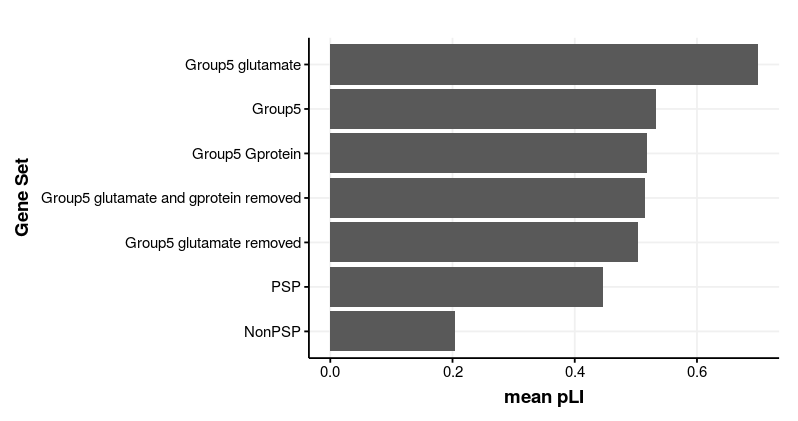
\includegraphics[width=\textwidth]{images/chapter_community_detection/ggplot2/pLI_group5_glutamate/Rplot_meanPLI.png}
    \caption{Mean pLI subgroups}
    \tiny\url{source('~/RProjects/chapter_community_detection/R/pLI _groups/plot/plot_pli_group5mean.R')}
    \label{fig:barplot pli mean subgroups group5}
\end{figure}

\begin{figure}
    \centering
    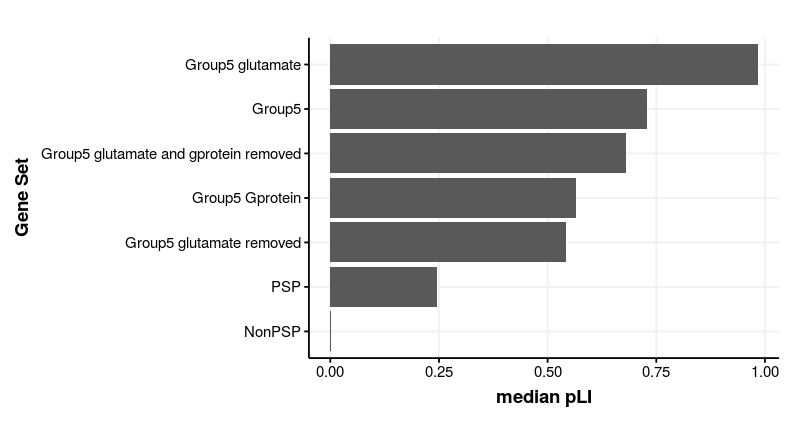
\includegraphics[width=\textwidth]{images/chapter_community_detection/ggplot2/pLI_group5_glutamate/Rplot_median_pLI.png}
    \caption{Median pLI subgroups}
    \tiny\url{source('~/RProjects/chapter_community_detection/R/pLI _groups/plot/plot_pli_group5median.R')}
    \label{fig:barplot pli median subgroups group5}
\end{figure}

% latex table generated in R 3.6.3 by xtable 1.8-4 package
% Sat Apr 24 14:30:23 2021
\begin{table}[ht]
\centering
\setlength{\extrarowheight}{2pt}
\begin{adjustbox}{width=\textwidth}
\begin{tabular}{lrrrrrrrr}
  \toprule
 & n & mean pLI & median & IQR & min & Q1 & Q3 & max \\ 
  \midrule
Group5 glutamate & 17 & 0.699 & 0.983 & 0.874 & $2.236 \times 10^{-13}$ & $1.245 \times 10^{-1}$ & 0.999 & 1.000 \\ 
  Group5 & 112 & 0.533 & 0.728 & 0.981 & $2.704 \times 10^{-26}$ & $5.619 \times 10^{-3}$ & 0.986 & 1.000 \\ 
  Group5 Gprotein & 38 & 0.519 & 0.566 & 0.949 & $1.125 \times 10^{-14}$ & $1.114 \times 10^{-2}$ & 0.960 & 1.000 \\ 
  G5 glutamate and gpr removed & 66 & 0.514 & 0.679 & 0.984 & $2.704 \times 10^{-26}$ & $4.928 \times 10^{-4}$ & 0.984 & 1.000 \\ 
  Group5 glutamate removed & 95 & 0.503 & 0.542 & 0.958 & $2.704 \times 10^{-26}$ & $1.479 \times 10^{-3}$ & 0.960 & 1.000 \\ 
  PSP & 3407 & 0.447 & 0.246 & 0.988 & $1.861 \times 10^{-164}$ & $3.118 \times 10^{-5}$ & 0.988 & 1.000 \\ 
  NonPSP & 14972 & 0.205 & 0.001 & 0.231 & $8.222 \times 10^{-118}$ & $2.068 \times 10^{-8}$ & 0.231 & 1.000 \\ 
   \bottomrule
\end{tabular}
\end{adjustbox}
\caption{Probability of loss of function intolerance in group 5} 
\label{tab:Probability of loss of function intolerance in group 5}
\end{table}



% latex table generated in R 3.6.3 by xtable 1.8-4 package
% Thu Apr  8 17:12:16 2021
\begin{table}[ht]
\centering
\setlength{\extrarowheight}{2pt}
\begin{tabular}{lrrrrr}
  \hline
 & group & mean & median & IQR & n \\ 
  \hline
1 & 55 & 0.6125448 & 0.9656300 & 0.9887303 & 43 \\ 
  2 & 24 & 0.6203871 & 0.9313400 & 0.9972226 & 75 \\ 
  3 & 43 & 0.6145202 & 0.8855300 & 0.9984190 & 144 \\ 
  4 & 53 & 0.5663651 & 0.8271400 & 0.9933349 & 402 \\ 
  5 & \textbf{5} & 0.5326375 & 0.7276050 & 0.9806836 & 112 \\ 
  6 & 33 & 0.5158691 & 0.6661800 & 0.9988866 & 188 \\ 
  7 & 20 & 0.5432248 & 0.6519100 & 0.9843646 & 147 \\ 
  8 & 16 & 0.4901432 & 0.5808950 & 0.9851005 & 72 \\ 
  9 & 34 & 0.4894469 & 0.5190200 & 0.9975823 & 211 \\ 
  10 & 26 & 0.4892552 & 0.5020700 & 0.9949257 & 119 \\ 
  11 & 23 & 0.4604868 & 0.3926700 & 0.9979424 & 72 \\ 
  12 & 32 & 0.4189881 & 0.2961600 & 0.9467203 & 52 \\ 
  13 & 2 & 0.4482511 & 0.2787300 & 0.9699159 & 158 \\ 
  14 & 11 & 0.4062157 & 0.1461250 & 0.9223713 & 56 \\ 
  15 & 6 & 0.3788960 & 0.1157750 & 0.9851261 & 78 \\ 
  16 & 46 & 0.4159553 & 0.1040850 & 0.9848124 & 48 \\ 
  17 & 44 & 0.3993356 & 0.0912190 & 0.9736422 & 102 \\ 
  18 & 1 & 0.4366882 & 0.0834400 & 0.9964374 & 170 \\ 
  19 & 7 & 0.3336776 & 0.0761265 & 0.7838825 & 128 \\ 
  20 & 12 & 0.3260981 & 0.0632415 & 0.7644625 & 34 \\ 
  21 & 28 & 0.4048670 & 0.0513270 & 0.9919099 & 37 \\ 
  22 & 22 & 0.3883770 & 0.0455180 & 0.9898240 & 42 \\ 
  23 & 58 & 0.3658420 & 0.0434000 & 0.9328980 & 35 \\ 
  24 & 3 & 0.3960078 & 0.0395070 & 0.9986700 & 41 \\ 
  25 & 10 & 0.3183102 & 0.0264130 & 0.7467980 & 153 \\ 
  26 & 47 & 0.4626781 & 0.0251515 & 0.9999640 & 26 \\ 
  27 & 17 & 0.3129865 & 0.0183380 & 0.7960093 & 145 \\ 
  28 & 51 & 0.3640889 & 0.0093548 & 0.9090049 & 111 \\ 
  29 & 45 & 0.3244065 & 0.0069318 & 0.8844465 & 121 \\ 
  30 & 25 & 0.2246596 & 0.0063216 & 0.1873631 & 27 \\ 
  31 & 19 & 0.2325151 & 0.0039051 & 0.5462425 & 20 \\ 
  32 & 9 & 0.2826638 & 0.0019705 & 0.8550521 & 62 \\
  33 & 4 & 0.2921367 & 0.0013367 & 0.6305098 & 31 \\ 
  34 & 48 & 0.1613250 & 0.0009721 & 0.0585315 & 23 \\ 
  35 & NON PSP  & 0.2045681 & 0.0006482 & 0.2312250 & 14972 \\ 
  36 & 62 & 0.2346489 & 0.0000584 & 0.1914650 & 34 \\ 
   \hline
\end{tabular}
\caption[Spectral groups ordered by pLI]{Rough table order by median PLI. Groups smaller than 15 filtered out for presentation}
\tiny\url{source('~/RProjects/chapter_community_detection/R/pLI _groups/pLI_across_groups.R')}
\label{tab: pli across groups}
\end{table}

\clearpage

60 terms in GO0007215:glutamate receptor signalling pathway bp
43 in PSP
17 in group 5 

28 of glutamate in GProtein
21 of glutamate in GProtein and PSP
9 of glutamate in Gprotein and group5


\todo{pLI for each group}

\subsection{Extra results:Remaining proteins after subgroup}
Remaining enrich for neurogenesis but the number of neurogenesis genes are low. Hill showed enrichement for neurogenesis genes but tested over 1000. Signal we have is from approx 7 and we also see enrichment in other areas close to glutamate synapses
check path to code2

\url{source('~/RProjects/go_analysis/R_src/GO_entity/load_neurogenesis.R')}

\url{source('~/RProjects/utils/src/generic_compile_gsa_neurogen.R')} MAC
This shows that there is not consistent enrichment for neurogenesis in group 5 22 genes associated with it 
\begin{table}[]
    \centering
    \begin{tabular}{lllllll}
        SET& NGENES&    BETA &BETA\_STD  &  SE      &   P  & P\_C\\
        \hline
  5  &   22&  0.2410&  0.00837& 0.237& 0.1537900& 0.0015956\\   
         & 
    \end{tabular}
    \caption{Intelligence neurogenesis}
    \label{tab:Intelligence neurogenesis}
\end{table}

\begin{table}[]
    \centering
    \begin{tabular}{lllllll}
        SET& NGENES&    BETA &BETA\_STD  &  SE      &   P  & P\_C\\
        \hline
  5   &  22&  0.7930&  0.027500& 0.242& 0.00052570 &0.1371100\\

 \end{tabular}
    \caption{Education neurogenesis}
    \label{tab:Education neurogenesis}
\end{table}

Group 36 enriches in all but EA3 but has only 4 neurogenesis genes \todo{What is enrichment in full gsa}





\subsection{Centrality measures for group 5}
\label{sec: centrality measures for group 5}

\begin{figure}
    \centering
    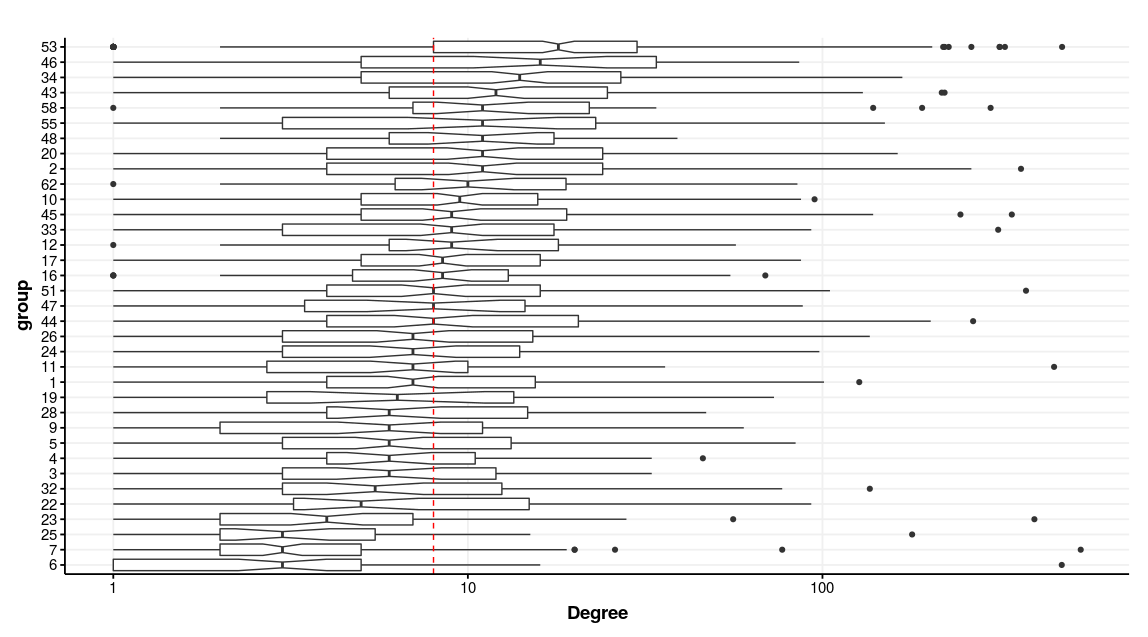
\includegraphics[width=\textwidth]{images/chaptercommunity/ggplot2/degreebygroup/Rplot_degree_theme_degree_label.png}
    \caption[Boxplot of degree grouped by spectral cluster]{Box plot of the degree distribution grouped by spectral clustering algorithm. Groups with less than fifteen members omitted. Red dashed line is median degree of nodes in PSP}
    \tiny\url{source('~/RProjects/chapter_community_detection/R/group5/degree/plot_histogram_degreebygroup.R')}
    \label{fig:my_label}
\end{figure}


The cohesive module that showed enrichment in the discovery and replication cohorts (group 5) had significantly lower mean closeness centrality (table~\ref{tab:closeness group 5}\footnote{\tiny\url{source('~/RProjects/chapter_community_detection/R/group5/degree/plot_histogram_closenessbygroup.R')}}) than the other groups and had the lowest eigenvector centrality (table~\ref{tab:eigenvector Wilcoxon}) which we have previously noted to be strongly correlated with being essential. Mean kcore was significantly lower (mean kcore=6.62) than the rest of the PSP after accounting for multiple comparisons (table~\ref{tab:kcoreness NOT logarithmic Wilcoxon}). Betweenness and degree centrality were not significantly different from other groups (table~\ref{tab:centrality_measures_for_group5}). At a group level group 5 possessed the network characteristics that are less associated with essentiality despite the high level of pLI (figure~\ref{fig:barplot pli mean subgroups group5}). Group 5 has a higher ranked pLI (table~\ref{tab: pli across groups}) but it's mean is not significantly different to the PSP as a whole (Wilcoxon rank sum test, W = 174,757, p-value = 0.3335). 

As the glutamate receptors have high pLI the others may have low or glutamate receptors may have low eig




\begin{table}[]
    \centering
    \setlength{\extrarowheight}{2pt}
    \begin{adjustbox}{width=\textwidth}
   
    \begin{tabular}{lllllllll}
    \toprule
    Centrality measure & $\mu_{k_C}$ & Median & $\delta \mu$     &$p$ & $p$ BH & $n$ & rank.sig  \\
    \midrule
    Closeness     &  0.0000917  & 0.0000921 &  -0.00000678 & $2.01\times10^{-9}$ &  $1.30\times 10^{-7}$    & 7 & 2 \\
    Degree   & 10.6875000 & 6.0000000 & -6.9567002 & $1.428 \times 10^{-2}$ & 0.79 & 7 & NS\\
    kcore &6.625 & 5.0 & -2.526 & $5.319 \times 10^{-4}$ & 0.03 & 10 & 10 \\  
    eigenvector & 0.0167635 & 0.0089846 & -0.0311651 & $8.827 \times 10^{-12}$ & $5.600 \times 10^{-10}$ & 16 & 2\\ 
    transitivity 0 & 0.117 & 0.0503507 & 0.008 & $4.206 \times 10^{-4}$ & $2.500 \times 10^{-2}$ & 9 & 7\\
    Betweenness&2272.6 & 247.42 & 1955.57 & $7.582 \times 10^{-1}$ & 1 & 4 & NS \\ 
    \bottomrule
    % latex table generated in R 3.6.3 by xtable 1.8-4 package
   \end{tabular}
    \end{adjustbox}
    \caption{Ranking of group 5 amongst 65 communities for centrality measures. Group 5 shows low eigenvector centrality and low closeness and belongs to an outer kcore - features that have been associated with less severe clinical phenotypes}
    \label{tab:centrality_measures_for_group5}
\end{table}




\section{Other community detection methods GSA}


Data for the performance of other community detection algorithms is provided for completeness. Full analysis including subgroup analysis is carried out for spectral clustering which appeared the most promising method. The second most attractive method was Louvain clustering which (excluding one group in infomap table~\ref{tab:Infomap Intelligence infomap significant in both groups}) is the only other group that showed significant enrichment in discovery and replication cohorts. 

Complete results for all clustering methods are provided in the supplemental material. 

\section{Louvain MAGMA GSA}
\label{sec: Louvain GSA}
Group 7 shows enrichment in the Intelligence\textsubscript{Discovery} sample (p=0.0012) and Intelligence\textsubscript{Replication} samples (p=0.0026) . Group 7 is composed of 154 genes but the number shown in the tables of results may be less than this if a gene was not assigned any SNPs using MAGMA. If we had used the Louvain algorithm in the same study design as the spectral method we would have taken forward groups 2,3,7 and 12 (considering only MAGMA) so the adjusted level of $\alpha$ for the Intelligence\textsubscript{Replication} sample would be 0.05/4= 0.0125. The significance of the replication enrichment is such that the significance level for group 7 Intelligence\textsubscript{Replication} is lower (p=0.0026) than the penalty for including all of the Louvain groups $\alpha$=0.00357 (0.05/14) (table~\ref{tab:louvain clustering intelligence}).

Group 7 is enriched for significant genes in the Educational attainment\textsubscript{Discovery} sample but not the replication cohort (p=0.0146 and replication p=0.4750 ; see table~\ref{tab:Louvain clustering Educational attainment phenotype}).



% latex table generated in R 3.6.1 by xtable 1.8-4 package
% Sat Mar 28 15:46:38 2020

\textbf{Group 7} is enriched for Molecular function \textbf{glutamate receptor activity} GO:0008066 	glutamate receptor activity (table~\ref{tab:Group 7 GO: Molecular Function 91 significant terms})






Bonferroni (against genome) $3.478 \times 10^{-32}$ 	Number in group 26  In annotation	84. 
Group 8 is large. The second most enriched Biological process is GO:0048666 \textbf{	neuron development} 		Bonferroni	$1.180 \times 10^{-52}$ 	Number in group 150 	Number in annotation 1298.\footnote{Code on mac\url{source('~/RProjects/utils/src/generic_compile_gsa_lourvain_new.R')}}
\todo{Overlap of group 7 with group 5}
\textbf{Takehome} second best guess we have also finds glutamate receptor clump that is enriched




% latex table generated in R 3.6.1 by xtable 1.8-4 packageXX
% Sun Apr 11 17:07:44 2021
\begin{table}[ht]
\centering
\setlength{\extrarowheight}{2pt}
\begin{tabular}{cllllllllll}
  \toprule
   &  \multicolumn{5}{c}{\textit{Discovery}} & \multicolumn{5}{c}{\textit{Replication}} \\
    \cmidrule{2-11}
Community & $n$ & $\beta$ & $\beta$ STD & SE & $p$ & $n$ & $\beta$ & $\beta$ STD & SE & $p$\\ 
  \midrule
1 & 196 & 0.10 & 0.01 & 0.07 & 0.0790 & 198 & -0.05 & -0.00 & 0.06 & 0.7749 \\ 
  2 & 334 & 0.09 & 0.01 & 0.05 & \textbf{0.0407} & 335 & 0.04 & 0.01 & 0.05 & 0.1916 \\ 
  3 & 510 & 0.10 & 0.02 & 0.04 & \textbf{0.0075} & 512 & 0.04 & 0.01 & 0.04 & 0.1006 \\ 
  4 & 245 & 0.06 & 0.01 & 0.06 & 0.1514 & 246 & 0.07 & 0.01 & 0.05 & 0.1053 \\ 
  5 & 112 & -0.08 & -0.01 & 0.09 & 0.8107 & 112 & 0.05 & 0.00 & 0.07 & 0.2525 \\ 
  6 & 159 & 0.12 & 0.01 & 0.07 & 0.0580 & 159 & 0.05 & 0.00 & 0.07 & 0.2284 \\ 
  \textbf{7} & 144 & 0.26 & 0.02 & 0.08 & \textbf{0.0012} & 144 & 0.21 & 0.02 & 0.07 & \textbf{0.0026} \\ 
  8 & 519 & 0.05 & 0.01 & 0.04 & 0.1103 & 519 & 0.07 &guess 0.01 & 0.04 & 0.0311 \\ 
  9 & 427 & 0.01 & 0.00 & 0.05 & 0.4054 & 428 & -0.02 & -0.00 & 0.04 & 0.6428 \\ 
  10 & 57 & 0.11 & 0.01 & 0.12 & 0.1910 & 57 & 0.01 & 0.00 & 0.11 & 0.4497 \\ 
  11 & 331 & -0.03 & -0.00 & 0.05 & 0.6911 & 332 & -0.00 & -0.00 & 0.05 & 0.5412 \\ 
  12 & 21 & 0.63 & 0.02 & 0.21 & \textbf{0.0014} & 21 & 0.17 & 0.01 & 0.17 & 0.1628 \\ 
  13 & 80 & -0.06 & -0.00 & 0.10 & 0.7250 & 80 & -0.03 & -0.00 & 0.09 & 0.6106 \\ 
  14 & 166 & 0.05 & 0.00 & 0.08 & 0.2554 & 166 & 0.17 & 0.02 & 0.07 & 0.0062 \\ 
   \bottomrule
\end{tabular}
\caption{Louvain clustering Intelligence phenotype} 
\label{tab:louvain clustering intelligence}
\tiny\url{source('~/RProjects/utils2/R/collate_results/generic_compile_gsa_lourvain.R')}
\end{table}
% ed


% % latex table generated in R 3.6.1 by xtable 1.8-4 package
% % Sun Apr 11 17:20:31 2021
% \begin{table}[ht]
% \centering
% \setlength{\extrarowheight}{2pt}
% \begin{tabular}{cllllllllll}
%   \toprule\setlength{\extrarowheight}{2pt}
%   &  \multicolumn{5}{c}{\textit{Discovery}} & \multicolumn{5}{c}{\textit{Replication}} \\
%     \cmidrule{2-11}
% Community & $n$ & $\beta$ & $\beta$ STD & SE & $p$ & $n$ & $\beta$ & $\beta$ STD & SE & $p$\\ 
%   \midrule
% 1 & 196 & 0.05 & 0.00 & 0.07 & 0.2610 & 194 & -0.02 & -0.00 & 0.06 & 0.5955 \\ 
%   2 & 334 & 0.13 & 0.02 & 0.05 & 0.0071 & 331 & 0.07 & 0.01 & 0.05 & 0.0568 \\ 
%   3 & 510 & 0.06 & 0.01 & 0.04 & 0.0878 & 508 & 0.04 & 0.01 & 0.04 & 0.1212 \\ 
%   4 & 245 & -0.04 & -0.00 & 0.06 & 0.7183 & 246 & 0.06 & 0.01 & 0.06 & 0.1351 \\ 
%   5 & 112 & 0.23 & 0.02 & 0.09 & 0.0063 & 111 & 0.03 & 0.00 & 0.08 & 0.3478 \\ 
%   6 & 159 & -0.04 & -0.00 & 0.08 & 0.6864 & 159 & 0.13 & 0.01 & 0.07 & 0.0343 \\ 
%   7 & 144 & 0.19 & 0.02 & 0.09 & 0.0146 & 144 & 0.00 & 0.00 & 0.08 & 0.4750 \\ 
%   8 & 519 & -0.01 & -0.00 & 0.04 & 0.5746 & 517 & 0.08 & 0.01 & 0.04 & 0.0259 \\ 
%   9 & 427 & 0.07 & 0.01 & 0.05 & 0.0849 & 425 & -0.01 & -0.00 & 0.05 & 0.6032 \\ 
%   10 & 57 & -0.19 & -0.01 & 0.13 & 0.9291 & 57 & 0.01 & 0.00 & 0.12 & 0.4783 \\ 
%   11 & 331 & 0.02 & 0.00 & 0.05 & 0.3721 & 328 & 0.00 & 0.00 & 0.05 & 0.4812 \\ 
%   12 & 21 & 0.08 & 0.00 & 0.21 & 0.3486 & 21 & -0.08 & -0.00 & 0.22 & 0.6508 \\ 
%   13 & 80 & 0.10 & 0.01 & 0.10 & 0.1623 & 79 & 0.00 & 0.00 & 0.10 & 0.4885 \\ 
%   14 & 166 & 0.00 & 0.00 & 0.08 & 0.4804 & 165 & 0.02 & 0.00 & 0.07 & 0.3795 \\ 
%   \bottomrule
% \end{tabular}
% \caption{Louvain clustering Educational attainment phenotype} 
% \tiny\url{source('~/RProjects/utils2/R/collate_results/generic_compile_gsa_lourvain.R')}
% \label{tab:Louvain clustering Educational attainment phenotype}
% \end{table}
% latex table generated in R 3.6.1 by xtable 1.8-4 package
% Sat Mar 28 15:49:04 2020
\clearpage


% Sun Apr 11 17:20:31 2021
\begin{table}[ht]
\centering
\setlength{\extrarowheight}{2pt}
\begin{tabular}{cllllllllll}
  \toprule
   &  \multicolumn{5}{c}{\textit{Discovery}} & \multicolumn{5}{c}{\textit{Replication}} \\
    \cmidrule{2-11}
Community & $n$ & $\beta$ & $\beta$ STD & SE & $p$ & $n$ & $\beta$ & $\beta$ STD & SE & $p$\\ 
  \midrule
1 & 196 & 0.05 & 0.00 & 0.07 & 0.2610 & 194 & -0.02 & -0.00 & 0.06 & 0.5955 \\ 
  2 & 334 & 0.13 & 0.02 & 0.05 & \textbf{0.0071} & 331 & 0.07 & 0.01 & 0.05 & 0.0568 \\ 
  3 & 510 & 0.06 & 0.01 & 0.04 & 0.0878 & 508 & 0.04 & 0.01 & 0.04 & 0.1212 \\ 
  4 & 245 & -0.04 & -0.00 & 0.06 & 0.7183 & 246 & 0.06 & 0.01 & 0.06 & 0.1351 \\ 
  5 & 112 & 0.23 & 0.02 & 0.09 & \textbf{0.0063} & 111 & 0.03 & 0.00 & 0.08 & 0.3478 \\ 
  6 & 159 & -0.04 & -0.00 & 0.08 & 0.6864 & 159 & 0.13 & 0.01 & 0.07 & 0.0343 \\ 
  7 & 144 & 0.19 & 0.02 & 0.09 & \textbf{0.0146} & 144 & 0.00 & 0.00 & 0.08 & 0.4750 \\ 
  8 & 519 & -0.01 & -0.00 & 0.04 & 0.5746 & 517 & 0.08 & 0.01 & 0.04 & 0.0259 \\ 
  9 & 427 & 0.07 & 0.01 & 0.05 & 0.0849 & 425 & -0.01 & -0.00 & 0.05 & 0.6032 \\ 
  10 & 57 & -0.19 & -0.01 & 0.13 & 0.9291 & 57 & 0.01 & 0.00 & 0.12 & 0.4783 \\ 
  11 & 331 & 0.02 & 0.00 & 0.05 & 0.3721 & 328 & 0.00 & 0.00 & 0.05 & 0.4812 \\ 
  12 & 21 & 0.08 & 0.00 & 0.21 & 0.3486 & 21 & -0.08 & -0.00 & 0.22 & 0.6508 \\ 
  13 & 80 & 0.10 & 0.01 & 0.10 & 0.1623 & 79 & 0.00 & 0.00 & 0.10 & 0.4885 \\ 
  14 & 166 & 0.00 & 0.00 & 0.08 & 0.4804 & 165 & 0.02 & 0.00 & 0.07 & 0.3795 \\ 
   \bottomrule
\end{tabular}
\caption{Louvain clustering Educational attainment phenotype. Sets 2,5 and 7 would be of interest but none are significant in the replication cohorts.} \tiny\url{source('~/RProjects/utils2/R/collate_results/generic_compile_gsa_lourvain.R')}
\label{tab:Louvain clustering Educational attainment phenotype}
\end{table}


% latex table generated in R 3.6.3 by xtable 1.8-4 package
% Sat Apr 24 13:35:54 2021
\begin{table}[ht]
\centering
\begin{adjustbox}{width=\textwidth}

\setlength{\extrarowheight}{2pt}
\begin{tabular}{llrrrr}
  \toprule
ID & Name & n & PSP & p & q FDR B.H \\ 
  \midrule
GO:0030165 & PDZ domain binding & 26 & 58 & $6.01 \times 10^{-21}$ & $2.75 \times 10^{-18}$ \\ 
  GO:0022803 & passive transmembrane transporter activi & 40 & 179 & $5.70 \times 10^{-19}$ & $8.70 \times 10^{-17}$ \\ 
  GO:0015267 & channel activity & 40 & 179 & $5.70 \times 10^{-19}$ & $8.70 \times 10^{-17}$ \\ 
  GO:0038023 & signaling receptor activity & 33 & 136 & $8.38 \times 10^{-17}$ & $7.67 \times 10^{-15}$ \\ 
  GO:0060089 & molecular transducer activity & 33 & 136 & $8.38 \times 10^{-17}$ & $7.67 \times 10^{-15}$ \\ 
  \textbf{GO:0008066} & glutamate receptor activity & 15 & 21 & $1.20 \times 10^{-16}$ & $9.14 \times 10^{-15}$ \\ \setlength{\extrarowheight}{2pt}
  GO:0022857 & transmembrane transporter activity & 47 & 292 & $3.49 \times 10^{-16}$ & $2.24 \times 10^{-14}$ \\ 
  GO:0046873 & metal ion transmembrane transporter acti & 34 & 152 & $3.97 \times 10^{-16}$ & $2.24 \times 10^{-14}$ \\ 
  GO:0022836 & gated channel activity & 28 & 100 & $4.40 \times 10^{-16}$ & $2.24 \times 10^{-14}$ \\ 
  GO:0005216 & ion channel activity & 35 & 163 & $5.33 \times 10^{-16}$ & $2.44 \times 10^{-14}$ \\ 
   \bottomrule
\end{tabular}
\end{adjustbox}
\caption{Group 7 Louvain GO: Molecular Function 91 significant terms} 
\tiny\url{source('~/RProjects/group_sizes/R/louvain_enrichment/group7_molecular_function.R')}
\label{tab:Group 7 GO: Molecular Function 91 significant terms}
\end{table}


% latex table generated in R 3.6.3 by xtable 1.8-4 package
% Sat Apr 24 13:48:00 2021
\begin{table}[ht]
\centering
\begin{tabular}{llrrrr}
  \toprule
ID & Name & n &  PSP & p & q FDR B.H \\ 
  \midrule
C0524528 & Pervasive Development Disorder & 22 & 113 & $2.87 \times 10^{-9}$ & $8.05 \times 10^{-6}$ \\ 
  C0004352 & Autistic Disorder & 36 & 285 & $5.26 \times 10^{-9}$ & $8.05 \times 10^{-6}$ \\ 
  C0036341 & Schizophrenia & 36 & 291 & $9.36 \times 10^{-9}$ & $9.56 \times 10^{-6}$ \\ 
  C1510586 & Autism Spectrum Disorders & 35 & 300 & $7.44 \times 10^{-8}$ & $5.70 \times 10^{-5}$ \\ 
  C1263846 & Attention deficit hyperactivity disorder & 23 & 152 & $1.82 \times 10^{-7}$ & $1.11 \times 10^{-4}$ \\ 
   \bottomrule
\end{tabular}
\caption{Group 7 Louvain Disease term enrichment Disease 74 significant terms} 
\label{tab:Group 7 Disease 74 significant terms}
\end{table}


\clearpage
\subsection{Result Infomap GSA}
\label{sec:result infomap gsa}
For intelligence cohort see table~\ref{tab:Infomap clustering Intelligence phenotype}. Only group 1 and 11 were significant in both groups. 

For education cohort see table~\ref{tab:Infomap clustering Educational attainment phenotype} None of those meeting size criteria showed enrichment in both discovery and replication samples. \ref{tab:infomap education}. For the large new cohorts in education (EA3) see table~\ref{tab:infomap EA3} and intelligence (Savage) see table~\ref{tab:Infomap savage}.

Group 11 consists of NMDA receptors and DLG genes. The disease most associated with it is ASD. Group 1 is large limiting enrichment analysis but RNA binding GO:0003723 in 406 genes P Bonferroni against all genome $2.728 \times 10^{-112}$ 


% latex table generated in R 3.6.1 by xtable 1.8-4 package
% Tue Mar 31 13:59:17 2020 int



% \begin{table}[ht]
% \centering
% \begin{tabular}{rlrrrrrr}
%   \hline
% + & SET & NGENES & BETA & BETA\_STD & SE & P & P\_C \\ 
%   \hline
% 1 & 1::: & 1176 & 0.1 & 0.02 & 0.03 & 0.0061 & 0.0479 \\ 
%   11 & 11::: & 47 & 0.4 & 0.02 & 0.15 & 0.0018 & 0.0080 \\ 
%   \hline
% \end{tabular}
% \caption{Intelligence infomap significant in both groups}
% \label{tab:Infomap Intelligence infomap significant in both groups}
% \end{table}



% latex table generated in R 3.6.1 by xtable 1.8-4 package
% Wed Apr 21 14:36:39 2021
\begin{table}[ht]
\centering
\setlength{\extrarowheight}{2pt}
\begin{tabular}{cllllllllll}
  \toprule
   &  \multicolumn{5}{c}{\textit{Discovery}} & \multicolumn{5}{c}{\textit{Replication}} \\
    \cmidrule{2-11}
Community & $n$ & $\beta$ & $\beta$ STD & SE & $p$ & $n$ & $\beta$ & $\beta$ STD & SE & $p$\\ 
  \midrule
1 & 1176 & 0.07 & 0.02 & 0.03 & 0.0061 & 1179 & 0.04 & 0.01 & 0.02 & 0.0479 \\ 
  8 & 62 & 0.24 & 0.01 & 0.13 & 0.0334 & 62 & -0.04 & -0.00 & 0.11 & 0.6540 \\ 
  9 & 48 & 0.35 & 0.02 & 0.14 & 0.0055 & 48 & -0.16 & -0.01 & 0.12 & 0.9143 \\ 
  11 & 47 & 0.44 & 0.02 & 0.15 & 0.0018 & 47 & 0.32 & 0.02 & 0.13 & 0.0080 \\ 
  24 & 20 & 0.42 & 0.01 & 0.24 & 0.0389 & 20 & 0.21 & 0.01 & 0.21 & 0.1610 \\ 
  27 & 17 & 0.38 & 0.01 & 0.23 & 0.0452 & 17 & -0.11 & -0.00 & 0.19 & 0.7238 \\ 
   \bottomrule
\end{tabular}
\caption{Infomap clustering Intelligence phenotype} 
\label{tab:Infomap clustering Intelligence phenotype}
\end{table}
% % latex table generated in R 3.6.1 by xtable 1.8-4 package
% % Tue Mar 31 14:07:01 2020
% \begin{table}[ht]
% \centering
% \begin{tabular}{rlrrrrrr}
%   \hline
%  & SET & NGENES & BETA & BETA\_STD & SE & P & P\_EA2 \\ 
%   \hline
% 99 & 99::: &  7 & 0.7 & 0.01 & 0.36 & 0.0211 & 0.0428 \\ 
%   106 & 106::: &  6 & 0.8 & 0.01 & 0.47 & 0.0452 & 0.0021 \\ 
%   135 & 135::: &  4 & 1.6 & 0.02 & 0.61 & 0.0038 & 0.0070 \\ 
%   \hline
% \end{tabular}
% \caption{Education infomap}
% \label{tab:infomap education}
% \end{table}
% % latex table generated in R 3.6.1 by xtable 1.8-4 package
% % Wed Apr 21 14:36:39 2021
\begin{table}[ht]
\centering
\setlength{\extrarowheight}{2pt}
\begin{tabular}{cllllllllll}
  \toprule
   &  \multicolumn{5}{c}{\textit{Discovery}} & \multicolumn{5}{c}{\textit{Replication}} \\
    \cmidrule{2-11}
Community & $n$ & $\beta$ & $\beta$ STD & SE & $p$ & $n$ & $\beta$ & $\beta$ STD & SE & $p$\\ 
  \midrule
8 & 62 & 0.31 & 0.02 & 0.13 & 0.0094 & 62 & -0.04 & -0.00 & 0.12 & 0.6365 \\ 
  19 & 26 & 0.36 & 0.01 & 0.21 & 0.0405 & 26 & -0.21 & -0.01 & 0.19 & 0.8638 \\ 
  21 & 22 & 0.38 & 0.01 & 0.21 & 0.0355 & 22 & 0.28 & 0.01 & 0.18 & 0.0623 \\ 
   \bottomrule
\end{tabular}
\caption{Infomap clustering Educational attainment phenotype} 
\label{tab:Infomap clustering Educational attainment phenotype}
\end{table}
\subsubsection{Markov clustering results}


No significant in both groups meeting size criteria tables in supplemental table~\ref{tab:MCL clustering Intelligence phenotype} and table~\ref{tab:Markov clustering Educational attainment phenotype}\footnote{\tiny \url{source('~/RProjects/utils2/R/collate_results/generic_compile_gsa_markov_cl.R')}}.

\subsubsection{Spinglass}
Nil significant

\url{source('~/RProjects/utils/src/generic_compile_gsa_sg1.R')}





 

\todo{what are setgenesout for all post synaptic or murine}

% % latex table generated in R 3.6.1 by xtable 1.8-4 packageXX
% % Sun Apr 11 17:07:44 2021
% \begin{table}[ht]
% \centering
% \setlength{\extrarowheight}{2pt}
% \begin{tabular}{cllllllllll}
%   \toprule
%   &  \multicolumn{5}{c}{\textit{Discovery}} & \multicolumn{5}{c}{\textit{Replication}} \\
%     \cmidrule{2-11}
% Community & $n$ & $\beta$ & $\beta$ STD & SE & $p$ & $n$ & $\beta$ & $\beta$ STD & SE & $p$\\ 
%   \midrule
% 1 & 196 & 0.10 & 0.01 & 0.07 & 0.0790 & 198 & -0.05 & -0.00 & 0.06 & 0.7749 \\ 
%   2 & 334 & 0.09 & 0.01 & 0.05 & 0.0407 & 335 & 0.04 & 0.01 & 0.05 & 0.1916 \\ 
%   3 & 510 & 0.10 & 0.02 & 0.04 & 0.0075 & 512 & 0.04 & 0.01 & 0.04 & 0.1006 \\ 
%   4 & 245 & 0.06 & 0.01 & 0.06 & 0.1514 & 246 & 0.07 & 0.01 & 0.05 & 0.1053 \\ 
%   5 & 112 & -0.08 & -0.01 & 0.09 & 0.8107 & 112 & 0.05 & 0.00 & 0.07 & 0.2525 \\ 
%   6 & 159 & 0.12 & 0.01 & 0.07 & 0.0580 & 159 & 0.05 & 0.00 & 0.07 & 0.2284 \\ 
%   7 & 144 & 0.26 & 0.02 & 0.08 & 0.0012 & 144 & 0.21 & 0.02 & 0.07 & 0.0026 \\ 
%   8 & 519 & 0.05 & 0.01 & 0.04 & 0.1103 & 519 & 0.07 & 0.01 & 0.04 & 0.0311 \\ 
%   9 & 427 & 0.01 & 0.00 & 0.05 & 0.4054 & 428 & -0.02 & -0.00 & 0.04 & 0.6428 \\ 
%   10 & 57 & 0.11 & 0.01 & 0.12 & 0.1910 & 57 & 0.01 & 0.00 & 0.11 & 0.4497 \\ 
%   11 & 331 & -0.03 & -0.00 & 0.05 & 0.6911 & 332 & -0.00 & -0.00 & 0.05 & 0.5412 \\ 
%   12 & 21 & 0.63 & 0.02 & 0.21 & 0.0014 & 21 & 0.17 & 0.01 & 0.17 & 0.1628 \\ 
%   13 & 80 & -0.06 & -0.00 & 0.10 & 0.7250 & 80 & -0.03 & -0.00 & 0.09 & 0.6106 \\ 
%   14 & 166 & 0.05 & 0.00 & 0.08 & 0.2554 & 166 & 0.17 & 0.02 & 0.07 & 0.0062 \\ 
%   \bottomrule
% \end{tabular}
% \caption{Louvain clustering Intelligence phenotype} 
% \label{tab:louvain clustering intelligence}
% \tiny\url{source('~/RProjects/utils2/R/collate_results/generic_compile_gsa_lourvain.R')}
% \end{table}
% % ed
% \section{To supplemental}

% \section{Continue}
% \textcolor{red}{graph partitioning bit removed commented out at this point}
% I hope to show the similarity and differences between using the graph Laplacian matrix and Modularity matrix for community detection and graph partitioning, in particular that they both use the graph spectra as solutions to optimisation problems (the minimisation of cut size and the maximisation of modularity). In the discussion that follows, I will use graph partitioning to mean separating a graph into two or more disjunct subgraphs in such a way that the minimum number of edges are cut. I will refer to community detection as finding disjunct sets of vertices that share more edges between them than would be expected at random, that is to say they are densely interconnected components.
% The two matrices that I will concentrate on are the Laplacian matrix L and the modularity matrix B.

% Several representations of the Laplacian matrix are used in the literature, often without further specification \cite{von2007tutorial}.The unnormalised graph Laplacian is defined:

% \begin{equation}
%     \mathbf{L} = \mathbf{D} - \mathbf{W}
% \end{equation}

% where $\mathbf{L}$ is the Laplacian, $\mathbf{D}$ is the diagonal degree matrix that has the degree of vertex i (the number of its connecting edges) at entry $\mathbf{D}_{i,i}$ and $\mathbf{W}$ as the weighted matrix.
% For our purposes the weight matrix will be the adjacency matrix $\mathbf{A}_{i,j}$ which has an entry
% 1 at $\mathbf{A}_{i,j}$ if there is an edge between vertex i and vertex j, and a zero otherwise.
% $\mathbf{A}$ will be symmetrical and the column and rows of $\mathbf{L}$ will add to zero. The vector 1 is
% therefore an eigenvector of L with eigenvalue zero as a linear combination of the columns
% of L is the zero vector.
% Two matrices are referred to as the normalised graph Laplacians. The symmetric:
    
% The symmteric:> 

% \begin{equation}
% {L}_{sym} = \mathbf{D}^{-\frac{1}{2}}\mathbf{L}\mathbf{D}^{-\frac{1}{2}}= \mathbf{I}-\mathbf{D}^{-frac{1}{2}}\mathbf{A}\mathbf{D}^{-\frac{1}{2}}
% \end{equation}

% and the random walk Laplacian:

% \begin{equation}
% \mathbf{L}_{rw}=\mathbf{D}^{-\frac{1}{2}}\mathbf{L}=\mathbf{I}-\mathbf{D}^{-\frac{1}{2}}\mathbf{A}
% \end{equation}

% We will make use of the fact that eigenvalues can represent a minimisation problem:

% \begin{equation}
% \lambda_{min}=\mathit{argmin}\frac{\mathbf{x}^T\mathbf{A}\mathbf{x}}{\mathbf{x}^T\mathbf{x}}
% \end{equation}

% %p29

% \begin{equation}
% R = \sum_{i,j}\mathbb{I}_{i,j\notin G_{same} }\mathbf{A}_{i,j}
% \end{equation}

% where there are two groups G. With this we count each edge twice so we should rescale R by 0.5.

% Defining an index vector $\mathbf{s}$ where $s_i$ is $+1$ if vertex $i$ is in group 1 and -1 if vertex $s_i$ is in group two, we can replace the indicator function,

% \begin{equation}
% \mathbb{I}_{i,j\notin samegroup}=\frac{1}{2}(1-s_i s_j)
% \end{equation}

% with,

% \begin{equation}
% R=\frac{1}{4}\sum_{i,j}(1-s_i s_j)\mathbf{A}_{i,j}
% \end{equation}

% \begin{equation}
% R = \frac{1}{4}\sum_{i,j}\mathbf{A}_{i,j}-s_i s_j \mathbf{A}_{i,j}
% \end{equation}

% Rewriting the first term in equation (here it is 7)

% \begin{equation}
% \sum_{i,j}\mathbf{A}_{i,j}=\sum_i k_i = \sum_i s_i ^2 k_i = \sum_{i,j} s_i s_j k_i \delta_{i,j}
% \end{equation}

% where $k_i$ is the degree of vertex $i$ and $s_i^2 = 1$ which is

% \begin{equation}
% R = \frac{1}{4}s_i s_j \sum_{i,j}(k_i \delta_{i,j} - \mathbf{A}_{i,j}
% \end{equation}


% from the definition of the degree matrix $\mathbf{D}$
% \begin{equation}
% \sum_{i,j} (\mathbf{D}_{i,j} -\mathbf{A}_{i,j} = \sum_{i,j} \mathbf{L}_{i,j}
% \end{equation}

% from the definition of the Laplacian in equation 5 (in document review)

% Including the group indicators $s_i$,$s_j$ as the vector $\mathbf{s}$ we have the quadratic form:
% \begin{equation}
% R=\frac{1}{4}\mathbf{s}^T\mathbf{L}\mathbf{s}
% \end{equation}

% so we want $\mathbf{s}$ such that we can minimise $R$. The factor of $\frac{1}{4}$ is irrelevant in the minimisation.

% The columns of the Laplacian sum to 0 which means that the vector $\mathbf{1}$ is in the nullspace of the columns of $\mathbf{l}$ and $R$ will be 0 when $\mat> hbf{x}$ is $\mathbf{1}$. The second smallest eigenvalue of $\mathbf{L}$, $\mathbf{x}$ will minimise $\mathbf{x^T}\mathbf{L}\mathbf{x}$.
% This is equivalent to minimising the cut size other than by the trivial solution of putting all the vertices in oune group. We can see that this minimises the sum of edges passing between two groups:

% \begin{equation}
% \mathbf{x^T}\mathbf{L}\mathbf{x}=\mathbf{x^T}\mathbf{D}\mathbf{x}-\mathbf{x^T}\mathbf{A}\mathbf{x}=\sum_i k_i x_i^2 = \sum_{i,j} A_{i,j}x_i x_j
% \end{equation}

% \begin{equation}
% \frac{1}{2}\sum_i d_i x_i^2 - 2 \sum_{i,j} x_i x_j A_{i,j} + k_jx_j^2)=\frac{1}{2}\sum{i,j}A_{i,j}(x_i - x_j)^2
% \end{equation}

% and $A_{i,j}$ is only equal to 1 if there is an edge between $A_{i,j}$.

% In order to forbid the trivial solution it is common to fix the size of the two groups. $R$ is then minimised by choosing $s$ to be proportional to the second eigenvector of the Laplacian. In most cases $s$ cannot be chosen parallel to $v$ so an approximation is made using the sign of the scond eigenvector eg if $v_i>=0$ then $s_i=0$.

% The disadvanges of this method, is that we must specify the community size and that minimising cut size does not always naturally yiled communitiues as we described in the section on maximising modularity.

